% ==============================================================================
% Universidade Federal do Rio Grande do Norte
% Centro de Tecnologia
% Programa de Pós-Graduação em Engenharia Elétrica e de Computação
% Qualificação
%
% Revisado em 12/07/2010 -- 10:00h
%
% Autor: Diogo Leite Rebouças <diogolr@gmail.com>
% ==============================================================================

% Classe .......................................................................
%\documentclass[a4paper,12pt,openright,twoside,notitlepage]{book}
\documentclass[a4paper,12pt,oneside,notitlepage]{book}

% Pacotes ......................................................................
% Pacotes Principais -----------------------------------------------------------
\usepackage[portuges,brazil]{babel}
\usepackage[utf8]{inputenc}

% Formatação de capítulos ------------------------------------------------------
%\usepackage[Sonny]{fncychap}
%\usepackage{fncychap}
\usepackage{capitulos}

% Figuras e Imagens ------------------------------------------------------------
\usepackage{graphicx}
% Figuras lado a lado
\usepackage{epsfig}
\usepackage{subfigure}

% Tikz
\usepackage{tikz}
\usepackage{pgfplots}
\pgfplotsset{compat=1.3}
\usepackage{tikz-timing}[2009/05/15]

% Utilizar H para inserir as imagens REALMENTE onde eu desejo
\usepackage{float}

% Fontes -----------------------------------------------------------------------
\usepackage[T1]{fontenc}
\usepackage{pslatex}

% Simbolos ---------------------------------------------------------------------
\usepackage{textcomp}

% Tabelas ----------------------------------------------------------------------
%\usepackage{multicol}
\usepackage{multirow}
% Colorir a tabela
\usepackage{colortbl}
% Tabelas com colunas de largura auto ajustável
\usepackage{tabularx}
% Notas de rodapé em tabelas (Pode-se usar o ambiente longtable também -
% Pesquisar exemplo com longtable)
\usepackage{threeparttable}

% Glossário --------------------------------------------------------------------
\usepackage[portuguese,noprefix]{nomencl}
\usepackage{makeglo}

% Outros pacotes ---------------------------------------------------------------
\usepackage{noitemsep}

% Comentários em bloco
\usepackage{verbatim}

% Hiperlinks
\usepackage{hyperref}

% Orientação de página
\usepackage{lscape}

% utilitários matemáticos
\usepackage{amsmath}
\usepackage{icomma}

% Referências ------------------------------------------------------------------
\usepackage[abbr]{harvard}	% As chamadas são sempre abreviadas
\harvardparenthesis{square}	% Colchetes nas chamadas
\harvardyearparenthesis{round}	% Parêntesis nos anos das referências
\renewcommand{\harvardand}{e}	% Substituir "&" por "e" nas referências


% Comandos .....................................................................
% Comandos gerais --------------------------------------------------------------
\newcommand{\titulo}{Título do trabalho grande o suficiente para ter uma ideia
                     do que irá acontecer na capa}
\newcommand{\autor}{Diogo Leite Rebouças}
\newcommand{\orientador}{Fábio Meneghetti Ugulino de Araújo}
\newcommand{\coorientador}{André Laurindo Maitelli}
\newcommand{\diaaprovacao}{26}
% Mês com inicial maiúscula (capa, folha de rosto)
\newcommand{\Mesaprovacao}{Julho}
% Mês com inicial minúscula (folha de assinaturas)
\newcommand{\mesaprovacao}{julho}
\newcommand{\anoaprovacao}{2010}
\let\Anoaprovacao\anoaprovacao
\newcommand{\dataaprovacao}{\diaaprovacao\ de \mesaprovacao\ de \anoaprovacao}

% Configuração da fonte
%\renewcommand{\familydefault}{\sfdefault}

% Margens ----------------------------------------------------------------------
\setlength{\oddsidemargin}{3.5cm}
\setlength{\evensidemargin}{2.5cm}
\setlength{\textwidth}{15cm}
\addtolength{\oddsidemargin}{-1in}
\addtolength{\evensidemargin}{-1in}

\setlength{\topmargin}{2.0cm}
\setlength{\headheight}{1.0cm}
\setlength{\headsep}{1.0cm}
\setlength{\textheight}{22.7cm}
\setlength{\footskip}{1.0cm}
\addtolength{\topmargin}{-1in}

% Glossário --------------------------------------------------------------------
\makeglossary

% Capítulos --------------------------------------------------------------------
% Não aparecer o número na primeira página dos capítulos
\newcommand{\mychapter}[1]{\chapter{#1}\thispagestyle{empty}}
\newcommand{\mychapterstar}[1]{\chapter*{#1}\thispagestyle{empty}}

% Comandos matemáticos ---------------------------------------------------------
% Implicação em fórmulas
\newcommand{\implica}{\quad\Rightarrow\quad} %Meio de linha
\newcommand{\implicafim}{\quad\Rightarrow}   %Fim de linha
\newcommand{\tende}{\rightarrow}

% Fração com parenteses
\newcommand{\pfrac}[2]{\parent{\frac{#1}{#2}}}

% Transformada de Laplace e transformada Z
\newcommand{\lapl}{\pounds}
\newcommand{\transfz}{\mathcal{Z}}

% Sequências
\newcommand{\sequencia}[4]{$#1_{#2}$, $#1_{#3}$, \ldots, $#1_{#4}$}

% Outros ----------------------------------------------------------------------
\newcommand{\chave}[1]{\left\{#1\right\}}
\newcommand{\colchete}[1]{\left[#1\right]}
\newcommand{\parent}[1]{\left(#1\right)}

% Hyperref ---------------------------------------------------------------------
\hypersetup{
    bookmarks=true,         % show bookmarks bar?
    unicode=false,          % non-Latin characters in Acrobat’s bookmarks
    pdftoolbar=true,        % show Acrobat’s toolbar?
    pdfmenubar=true,        % show Acrobat’s menu?
    pdffitwindow=false,     % window fit to page when opened
    pdfstartview={FitH},    % fits the width of the page to the window
    pdftitle={\titulo},     % title
    pdfauthor={\autor},     % author
    pdfsubject={mestrado},  % subject of the document
    pdfcreator={\autor},    % creator of the document
    pdfproducer={\autor},   % producer of the document
    pdfkeywords={Controle}, % list of keywords
    pdfnewwindow=true,      % links in new window
    colorlinks=false,       % false: boxed links; true: colored links
    linkcolor=black,        % color of internal links
    citecolor=black,        % color of links to bibliography
    filecolor=black,        % color of file links
    urlcolor=black          % color of external links
}


% Inicio do documento ..........................................................
\begin{document}

\pagestyle{empty}

\begin{titlepage}
\begin{center}

\begin{tabularx}{\linewidth}{@{}lcr@{}}
% Primeira Linha
\multirow{4}{*}{
\includegraphics[width=3cm]{imgs/outras/eps/ufrn_trad}}&
\textsc{Universidade Federal do Rio Grande do Norte} &
\multirow{4}{*}{
\includegraphics[width=2cm]{imgs/outras/eps/ppgeec}}\\
% Segunda Linha
& 
\textsc{Centro de Tecnologia}
&\\
% Terceira Linha
& 
\textsc{Programa de Pós-graduação em Engenharia}
&\\
% Quarta Linha
& 
\textsc{Elétrica e de Computação}
&
\end{tabularx}

\vfill

\LARGE
\textbf{\titulo}

\vfill

\Large
\textbf{\autor}

\vfill
\large
\textbf{Natal -- RN\\\Mesaprovacao\ /\ \Anoaprovacao}

\end{center}
\end{titlepage}

\begin{titlepage}
\begin{center}

\LARGE
\textbf{\titulo}

\vfill

\Large
\textbf{\autor}

\vfill

\normalsize
Orientador: Prof. Dr. \orientador
%\\[2ex] Co orientador: Prof. Dr. \coorientador

\vfill

\hfill
\parbox{0.5\linewidth}{\textbf{\documento} apresentada ao Programa
de Pós-graduação em Engenharia Elétrica e de Computação da UFRN (área de
concentração: Automação e Sistemas) como parte dos requisitos para obtenção do
título de Mestre em Ciências.}

\vfill

\large
\textbf{Natal, RN, \Mesaprovacao\ de \Anoaprovacao}

\end{center}

\end{titlepage}

%\newpage

\begin{center}

% Aqui não se usou \vfill porque o \vfill é construído internamente com
% o comando \vspace. Espaços verticais no início da folha com \vspace
% são ignorados. Para que isto não ocorra deve-se usar o \vspace*
% \vspace*{\fill} é como se fosse um \vfill*
\vspace*{\fill}

Divisão de Serviços Técnicos\\[1ex]
Catalogação da publicação na fonte.
UFRN / Biblioteca Central Zila Mamede

\vspace{2ex}

\begin{tabular}{|p{0.9\linewidth}|} \hline
\\
Rebouças, Diogo Leite.\\
\hspace{1em} Sobre a Preparação de Propostas de Tema, Dissertações
e Teses no Programa de Pós-Graduação em Engenharia Elétrica e 
Computação da UFRN / Fulano dos Anzóis Pereira - Natal, RN, 2010 \\
\hspace{1em} XYZ p. \\
\\
\hspace{1em} Orientador: \orientador \\
\hspace{1em} Co-orientador: \coorientador \\
\\
\hspace{1em} Dissertação de mestrado - Universidade Federal do Rio Grande do
Norte.  Centro de Tecnologia. Programa de Pós-Graduação em Engenharia Elétrica e
Computação.
\\
\\
\hspace{1em} 1. Redação técnica - Dissertação. 2. \LaTeX - Tese.
I. Araújo, Fábio Meneghetti Ugulino de. II. Meitelli, André Laurindo.
III. Título. \\
\\
RN/UF/BCZM \hfill CDU 004.932(043.2) \\ \hline
\end{tabular} 

\end{center}

\begin{titlepage}
\begin{center}

\LARGE

\textbf{\titulo}

\vfill

\Large

\textbf{\autor}

\end{center}

\vfill

\noindent
\documento\ aprovada em \dataaprovacao\ pela banca examinadora composta pelos
seguintes membros:

\begin{center}

% Abreviaturas -----------------------------------------------------------------
% Doutor = Dr.
% Doutora = Dr\textordfeminine.
% Mestre = Me.
% Mestra = Ma.

\vspace{1.5cm}\rule{0.95\linewidth}{1pt}
\parbox{0.9\linewidth}{%
Prof. Dr. \orientador\ (Orientador) \dotfill\ DCA/UFRN}

\vspace{1.5cm}\rule{0.95\linewidth}{1pt}
\parbox{0.9\linewidth}{%
%Prof. Dr. \coorientador (Co-orientador) \dotfill\ DCA/UFRN}
Prof. Dr. André Laurindo Maitelli (Examinador Interno)\ \dotfill\ DCA/UFRN}

\vspace{1.5cm}\rule{0.95\linewidth}{1pt}
\parbox{0.9\linewidth}{%
Prof. Dr. Oscar Gabriel Filho (Examinador Externo)\ \dotfill\ UnP}

\end{center}
\end{titlepage}

%\begin{titlepage}

\vspace*{\fill}

\hfill
\begin{minipage}{0.5\linewidth}
\begin{flushright}
\large\it
``Algo só é impossível até que alguém duvide e acabe provando o
contrário.''\linebreak
\small
Sir Albert Einstein
\end{flushright}
\end{minipage}

\end{titlepage}

%\begin{titlepage}

\vspace*{\fill}

\hfill
\begin{minipage}{0.5\linewidth}
\begin{flushright}
\large\it
Dedico este trabalho primeiramente a Deus, que me confortou nos momentos mais
difíceis e que indicou o caminho certo ao longo de toda minha vida. Ao meu anjo
da guarda, pela proteção e iluminação. À toda minha família e, em especial, aos
meus pais, Marcondes e Aretusa, pela compreensão e dedicação ao longo desta e de
outras jornadas. À minha namorada pelo apoio e incentivo durante a realização
deste trabalho. Que não lhes falte saúde, paz e tranquilidade. Fica aqui minha
gratidão eterna, pois sem vocês nada seria possível.
\end{flushright}
\end{minipage}

\vspace*{\fill}

\end{titlepage}

%\chapter*{Agradecimentos}
\thispagestyle{empty}

\begin{trivlist}  \itemsep 2ex

\item Aos meus pais, pelo incentivo aos estudos ao longo de toda minha vida. Sem
vocês eu não seria nada.

\item A minha namorada, pela paciência, apoio e compreensão nas horas em que eu
precisei me ausentar, em benefício deste e de outros tantos trabalhos durante
esses anos. Sem você, talvez eu não tivesse conseguido.

\item Ao meu orientador, professor Fábio Meneghetti Ugulino de Araújo, sou grato
pela orientação.

\item Aos professores André Laurindo Maitelli e Carlos Eduardo Trabuco Dórea,
pelas contribuições durante o exame de qualificação.

\item Aos colegas de pós-graduação, pelas críticas e sugestões.

\item À todos os professores e funcionários do Departamento de Engenharia de
Computação e Automação e do Programa de Pós-Graduação em Engenharia Elétrica e
de Computação, pelo aprendizado e pela ajuda.

\item Ao professor Adelardo Adelino Dantas de Medeiros, por ter desenvolvido o
modelo de tese do Programa de Pós Graduação em Engenharia Elétrica e de
Computação.

\item Aos integrantes do projeto Pró-Engenharias da UFRN, do ITA e da UFPA.

\item À CAPES, pelo apoio financeiro.

\end{trivlist}

\mychapterstar{Resumo}
Em um processo real, todos os recursos utilizados, sejam físicos ou
desenvolvidos em {\it software}, estão sujeitos a interrupções ou a
comprometimentos operacionais. Contudo, nas situações em que operam os sistemas
críticos, qualquer tipo de problema pode vir a trazer grandes consequências.
Sabendo disso, este trabalho se propõe a desenvolver um sistema capaz de
detectar a presença e indicar os tipos de falhas que venham a ocorrer em um
determinado processo. Para implementação e testes da metodologia proposta, um
sistema de tanques acoplados foi escolhido como modelo de estudo de caso. O
sistema a ser desenvolvido deverá gerar um conjunto de sinais que notifiquem o
operador do processo e que possam vir a ser pós-processados, possibilitando que
sejam feitas alterações nas estratégias ou nos parâmetros dos controladores. Em
virtude dos riscos envolvidos com relação à queima dos sensores, atuadores e
amplificadores existentes na planta real, o conjunto de dados das falhas serão
gerados computacionalmente e os resultados serão coletados a partir de
simulações numéricas do modelo do processo, não havendo risco de dano aos
equipamentos. O sistema será composto por estruturas que fazem uso de Redes
Neurais Artificiais, treinadas em modo {\it offline} pelo {\it software}
matemático Matlab\reg.

\vspace{1.5ex}

\noindent {\bf Palavras-chave}: Sistemas Críticos, Detecção de Falhas, Diagnóstico de
Falhas, Redes Neurais Artificiais.

\mychapterstar{Abstract}
In a real process, all used resources, whether physical or developed in
software, are subject to interruptions or operational commitments. However, in
situations in which operate critical systems, any kind of problem may bring big
consequences. Knowing this, this paper aims to develop a system capable to
detect the presence and indicate the types of failures that may occur in a
process. For implementing and testing the proposed methodology, a
coupled tank system was used as a study model case. The system should be
developed to generate a set of signals that notify the process operator and that
may be post-processed, enabling changes in control strategy or control
parameters. Due to the damage risks involved with sensors, actuators and
amplifiers of the real plant, the data set of the faults are generated
computationally and the results will be collected from numerical simulations of
the process model. At the end, there will be a comparative analysis of two
proposed fault detection and diagnosis systems. In both cases the system will be
composed by structures with Artificial Neural Networks.

\vspace{1.5ex}

\noindent {\bf Keywords}: Critical Systems, Fault Detection, Fault Diagnosis,
Artificial Neural Network.


\frontmatter

\addcontentsline{toc}{chapter}{Sumário}
\tableofcontents

\cleardoublepage
\addcontentsline{toc}{chapter}{Lista de Figuras}
\listoffigures

\cleardoublepage
\addcontentsline{toc}{chapter}{Lista de Tabelas}
\listoftables

\cleardoublepage
\renewcommand{\nomname}{Lista de Símbolos e Abreviaturas}
\renewcommand{\glossaryname}{\nomname}
\markboth{\MakeUppercase{\nomname}}{\MakeUppercase{\nomname}}
\addcontentsline{toc}{chapter}{\nomname}
\printglossary

\mainmatter

% Capítulos ....................................................................
\pagestyle{headings}

\mychapter{Introdução}
\label{cap:introducao}

Segundo \citeasnoun{ribeiro:1999}, o termo automação está relacionado com a
substituição da mão-de-obra humana ou animal por uma máquina que realize função
equivalente. Partindo desse princípio, pode-se dizer que a automação surge na
sociedade em meados do século X, com os moinhos hidráulicos que produziam
farinha. Tal mecanismo, capaz de substituir o trabalho de dez a vinte homens,
fez com que a produção de alimentos passasse por uma fase de crescimento nunca
antes observada.

Desde então, o homem tem direcionado seu conhecimento para o desenvolvimento de
tecnologias que o auxiliem em suas atividades. Com a revolução industrial, a
partir da segunda metade do século XVIII, o processo de transformação e
desenvolvimento dessas tecnologias foi acelerado, de tal forma que o homem foi
capaz de produzir uma máquina a vapor para movimentar equipamentos industriais e
de fazer um martelo de 60 quilos dar 150 golpes por minuto \cite{goeking:2010}.

Por outro lado, a utilização de sistemas de controle remete a tempos ainda mais
antigos, por volta de 300 a.C. a 250 a.C., quando foram desenvolvidas as
primeiras bóias flutuadoras, o relógio de água de Ktesíbios e uma lamparina a
óleo que matinha o nível de óleo combustível constante
\cite{mayr:1970,mayr:1971,mayr:1975}.

Já na Europa Moderna, o primeiro sistema com realimentação a ser inventado foi o
regulador de temperatura de Cornelis Drebbel, entre o final do século XVI e
início do século XVII \cite{mayr:1975}. No final do século XVII e início do
século XVIII, Dennis Papin inventou o primeiro regulador de pressão para
caldeiras a vapor. Tal dispositivo tinha funcionalidade semelhante a uma válvula
de segurança de uma panela de pressão \cite{dorf:2009}. 

% ------------------------------------------------------------------------------
\section{Aspectos históricos do controle automático}
A junção dos conceitos de automação e sistemas de controle se dá no final do
século XVIII, quando, em 1769, James Watt desenvolve o primeiro controlador
automático com realimentação usado em um processo industrial, conhecido como
{\it regulador de esferas}.

\begin{comment}
O dispositivo, inteiramente mecânico, mostrado na Fig.
\ref{fig:controlador_james}, controlava a velocidade de um motor a vapor através
do movimento de duas esferas. Na medida em que a velocidade do eixo de saída do
motor a vapor aumentava, as esferas eram elevadas (por força centrífuga) e a
válvula era fechada, diminuindo o fluxo de vapor para o motor e,
consequentemente, sua velocidade. No caso oposto, quando a velocidade de saída
do eixo do motor a vapor reduzia, as esferas eram rebaixadas, abrindo a válvula
e aumentando o fluxo de vapor para o motor, o que, consequentemente, aumentava
sua velocidade \cite{mayr:1970,mayr:1975,dorf:2009}.

\begin{figure}[htb]
\centering
    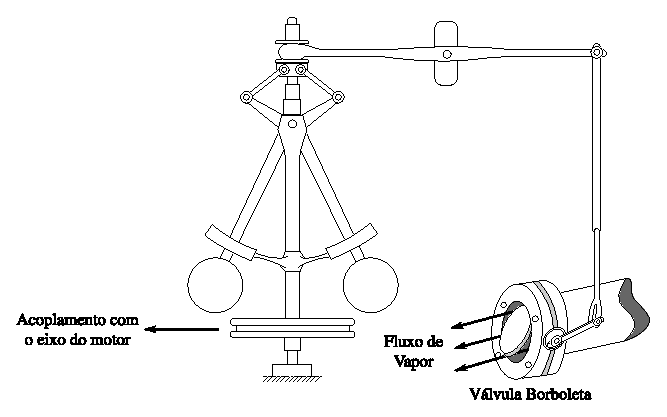
\includegraphics{imgs/introducao/eps/regulador_esferas}
    \caption{Regulador de Esferas de James Watt.}
    \label{fig:controlador_james}
\end{figure}

\end{comment}

Ainda em 1769, segundo \citeasnoun{faccin:2004}, Richard Arkwright, um inventor
inglês considerado um dos precursores das técnicas de produção em série,
acelerou o processo de industrialização ao desenvolver uma máquina de tecer
movimentada pela força da água corrente. 

Segundo o autor, foi o tear mecânico que impulsionou a Revolução Industrial na
Europa, contribuindo diretamente para a mudança dos hábitos de trabalho e das
relações sociais da Idade Contemporânea. 

De acordo com \citeasnoun{dorf:2009}, o século seguinte foi caracterizado pelo
desenvolvimento de sistemas de controle automático através da intuição e da
invenção. Esforços para aumentar a exatidão dos sistemas de controle levaram a
atenuações mais lentas das oscilações transitórias e até mesmo a sistemas
instáveis, tornando-se necessário o desenvolvimento da teoria de controle
automático.

Por volta de 1868, J. C. Maxwell formulou a teoria matemática, através das
equações diferenciais do regulador de esferas de James Watt, relacionando os
efeitos dos parâmetros do sistema com o seu desempenho \cite{maxwell:1964}. Com
o seu trabalho, Maxwell demonstrou a importância e a utilidade de modelos e
métodos matemáticos para a compreensão dos processos industriais e da teoria de
controle.

Nos anos seguintes, E. J. Routh (1877) e A. Hurwitz (1885) criaram seus
critérios de estabilidade de maneira independente
\cite{routh:1877,bennett:1996}. Mais tarde, em 1896, A. M. Lyapunov também
desenvolveu seu critério de estabilidade baseado em equações diferenciais
não-lineares de movimento \cite{faccin:2004}.

No início do século XX, por volta de 1907, foi desenvolvido o primeiro
controlador de temperatura pneumático (do tipo liga-desliga), o qual foi
instalado em uma unidade de pasteurização de leite em Nova York. Poucos anos
depois, em 1914, Edgar H. Bristol, fundador da {\it Foxboro Instrument Company},
contribuiu significativamente para o desenvolvimento de sistemas de controle ao
protocolar o pedido de patente de um amplificador denominado {\it flapper-nozzle
amplifier}, capaz de prover a ação proporcional. Em seguida, por volta de 1920,
Morris E. Leeds obteve uma patente de um controlador eletromecânico que provia a
ação integral \cite{faccin:2004}.

Em 1922, Nicholas Minorsky apresentou uma análise sobre a teoria de controle
envolvida no controle de posição, formulando a lei de controle de três termos,
hoje conhecida como controle PID.  Entretanto, até 1930 seu trabalho não havia
sido amplamente reconhecido \cite{bennett:1996}.

Somente em 1935, Ralph Clarridge criou o controlador de três termos, ao utilizar
um controlador que antecipava a variação no sinal de erro para solucionar um
problema de oscilação de uma malha de controle de temperatura em uma indústria
de celulose \cite{faccin:2004}.

% ------------------------------------------------------------------------------
\section{Introdução da automação na indústria}
Durante o período entre guerras, a teoria e a prática de sistemas de controle
nos Estados Unidos e na Europa Ocidental se desenvolveram de modo diferente do
que na Rússia e no Leste Europeu. O principal incentivo para o uso da
realimentação nos Estados Unidos foi o desenvolvimento do sistema telefônico e
dos amplificadores eletrônicos com realimentação por Bode, Nyquist e Black nos
Laboratórios Telefônicos Bell \cite{dorf:2009}.

Durante a segunda guerra mundial fez-se necessário projetar e construir pilotos
automáticos para aeronaves, sistemas de posicionamento de armas, sistemas de
controle de antenas de radares e outros sistemas militares baseados na abordagem
do controle com realimentação. A complexidade e o desempenho esperados desses
sistemas militares fizeram com que houvesse uma extensão das técnicas de
controle disponíveis além de promoverem o interesse em sistemas de controle e o
desenvolvimento de novos critérios e métodos. O projeto de sistemas de controle,
até então, era uma arte envolvendo a abordagem da tentativa e erro
\cite{dorf:2009}.

A primeira tentativa de sucesso que não levava em consideração métodos de
tentativa e erro foi proposta em \citeasnoun{ziegler:1942}. Neste artigo, foram
apresentados dois procedimentos para sintonia dos controladores através de
regras simples baseadas nas características dinâmicas do processo.

Após a disseminação dos controladores PID na industria nos anos seguintes à
publicação do artigo de Ziegler e Nichols, aconteceu o grande marco da indústria
eletrônica: a criação, em 1947, do transistor. A partir de então, começaram a
ser desenvolvidos os primeiros ``computadores industriais''. Segundo
\citeasnoun{goeking:2010}, embora o microprocessamento tenha sido comercializado
apenas a partir da década de 60, foi nesse período que surgiram os primeiros
robôs mecânicos que incorporavam os sistemas de microprocessamento e uniam
tecnologias mecânicas e elétricas.

Considerando que até o final da década de 60, as empresas automobilísticas,
apesar de produzirem em grande escala com rapidez e qualidade, não ofereciam
muitas opções de personalização para os clientes (incluindo as cores dos
acessórios), a General Motors, solicitou à empresa Allen-Bradley que
confeccionasse um produto que conferisse versatilidade à produção. A empresa que
já produzia outros dispositivos elétricos, desenvolveu em 1968, o primeiro
Controlador Lógico Programável (CLP), substituindo os antigos painéis de relés,
permitindo fazer modificações rápidas no processo produtivo \cite{goeking:2010}.

\Glossary{CLP}{Controlador Lógico Programável}

De acordo com \citeasnoun{isermann:2006}, a partir de 1975, com a
disponibilidade de microcomputadores ``baratos'', o grau de automação da
industria foi drasticamente elevado. Tal aumento ocorreu em paralelo com os
avanços dos sensores, atuadores, das redes de comunicação e das Interfaces
Humano-Computador (IHC).

\Glossary{IHC}{Interface Humano-Computador}

Desde então, a demanda cada vez mais crescente pela necessidade de maior
desempenho dos processos ou de maior qualidade dos produtos, bem como a
independência do funcionamento da planta para com os operadores humanos, vem
despertando interesse de diversos membros da comunidade científica.

%TODO citar artigos de pesquisas na área de controle/desempenho do
%processo/qualidade dos produtos

% ------------------------------------------------------------------------------
\section{A automação e supervisão de processos}
A Fig. \ref{fig:esquema_automacao} mostra um esquema simplificado da automação
de dois processos acoplados. O esquema foi dividido em três níveis: nível
inferior, o qual contempla as estratégias de controle mais comuns na industria;
nível intermediário, onde estarão os sistemas de supervisão e o nível superior,
no qual estão contidas as atividades de gerenciamento, coordenação e otimização
dos processos.

\begin{figure}[!htb]
\centering
    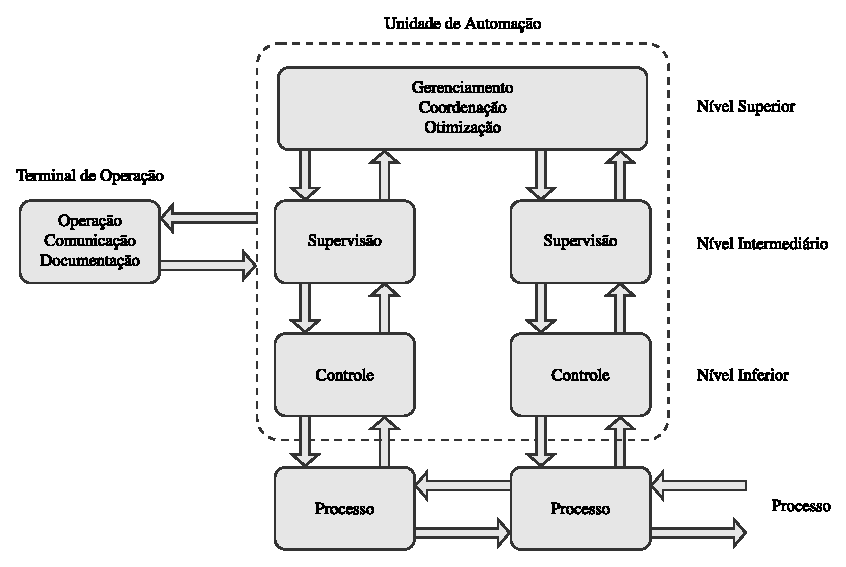
\includegraphics{imgs/introducao/eps/esquema_automacao}
    \caption{Diagrama esquemático da automação de dois processos acoplados.}
    \label{fig:esquema_automacao}
\end{figure}

Segundo com \citeasnoun{isermann:2006}, ao longo dos anos diversos estudos foram
desenvolvidos sobre a teoria de controle com realimentação.  Especialmente nos
sistemas de controle que incluem os observadores de estado e estimadores de
parâmetros, pode-se observar uma evolução significativa. Para o autor, com a
evolução da teoria de controle e de processamento de sinais, diversos processos
que antes possuíam um comportamento que dificultava a elaboração de estratégias
de controle, agora podem ser controlados mais facilmente.

Entretanto, quanto mais eficiente forem as estratégias de controle no nível
inferior, melhor deverão ser as estratégias de supervisão do nível
intermediário, uma vez que os operadores são removidos do processo. Pode-se
dizer que isso ocorre porque os operadores humanos não se limitam a controlar o
processo mudando suas referências nos horários previstos, eles também realizam
a atividade de supervisão, especialmente quando estão em contato direto com o
processo. Logo, com a evolução das técnicas de controle no nível inferior, as
estratégias de supervisão também deverão ser aperfeiçoadas.

No passado, o supervisionamento automático dos processos, em sua maioria, era
composto por algum tipo de sistema que possuía a simples tarefa de verificar se
uma determinada variável, tal como {\it força}, {\it velocidade}, {\it pressão},
{\it nível} ou {\it temperatura}, ultrapassava um certo limite ou limiar
especificado para o processo. Caso isso viesse a ocorrer, um tipo de alarme
disparava, notificando o operador do ocorrido, fazendo com que este agisse de
maneira a corrigir o problema. Algumas vezes o problema podia ser corrigido
também de maneira automática por algum subsistema de proteção. Tal procedimento,
em muitos dos casos, era suficiente para evitar que houvessem falhas ou danos
graves ao processo. Por outro lado, as falhas ou os erros só eram detectados
após um certo intervalo de tempo, o que impossibilitava a obtenção de um
diagnóstico detalhado sobre o ocorrido \cite{isermann:2006}.

Os desafios desse segmento estão, portanto, em se utilizar modelos matemáticos
do processo, modelos de sinais, métodos de identificação e estimação e técnicas
de inteligência artificial para se desenvolver um sistema capaz de detectar e
diagnosticar falhas em um processo. Para se desenvolver esses tipos de sistemas,
deve-se levar em consideração diversos aspectos, destacando-se: a detecção
antecipada de pequenas falhas (abruptas ou incipientes); o diagnóstico de falhas
nos sensores, atuadores e componentes de um processo; o supervisionamento de
estados transientes; o reparo e a manutenção baseados no comportamento do
processo; o rigoroso controle de qualidade em processos de fabricação; a
detecção e diagnóstico de falhas remotas; o suporte para gerenciamento de falhas
e o suporte para sistemas tolerantes a falhas e sistemas reconfiguráveis.

Considerando tais aspectos, pode-se dizer que as primeiras publicações na área
de Detecção e Diagnóstico de Falhas (DDF) estão relacionadas com sistemas
aeroespaciais \cite{beard:1971,jones:1973,willsky:1976,clark:1978} e processos
químicos \cite{himmelblau:1978}. Os primeiros conceitos discutidos podem ser
classificados como abordagens de relação de paridade. Em tais documentos são
demonstrados procedimentos de verificação da consistência da leitura dos
instrumentos ou do balanço de massas. Outras abordagens, as quais utilizavam o
erro residual do balanço de massas foram aplicadas, por exemplo, na verificação
de vazamento em dutos \cite{billman:1987}. A abordagem de relações de paridade
foi também investigada em \citeasnoun{gertler:1985}.

\Glossary{DDF}{Detecção e Diagnóstico de Falha}

Nessa mesma época, também foram desenvolvidos métodos baseados em observadores
de estado ou filtros de Kalman \cite{beard:1971,mehra:1971,jones:1973}. Em
\citeasnoun{clark:1978}, por exemplo, um banco de observadores é utilizado para
detectar falhas em sensores através de redundância de informações. Uma variação
dos modelos de observadores de estado foi mostrada em \citeasnoun{patton:1991},
no qual se faz uso de uma estrutura de autovalores e autovetores para detecção
de falhas.

Uma outra abordagem para esse tipo de sistema fez uso de estimadores de
parâmetros, como pode ser observado em \citeasnoun{baskiotis:1979} para
aplicações com turbinas de aeronaves, em \citeasnoun{isermann:1982},
\citeasnoun{isermann:1984} e \citeasnoun{isermann:1993} para processos de
maneira geral, bombas e motores de corrente contínua, ou ainda em
\citeasnoun{filbert:1982} e \citeasnoun{filbert:1985} para aplicações envolvendo
motores elétricos.

Mais recentemente, diversas contribuições foram feitas na área de DDF. Pode-se
citar, por exemplo, as publicações relacionadas ao gerenciamento de falhas e
supervisão de processos, tais como \citeasnoun{russel:2000},
\citeasnoun{patton:2000}, \citeasnoun{higham:2001}, \citeasnoun{simani:2003},
\citeasnoun{ericson:2005}, \citeasnoun{blanke:2006}, \citeasnoun{erdenet:2007},
\citeasnoun{fesq:2009} e \citeasnoun{hang:2009}.

Uma outra contribuição importante é mostrada em \citeasnoun{vdi2206:2003}, no
qual é exposto um ``Diagrama em V'', que lista passos importantes para o
desenvolvimento de sistemas de DDF.  \citeasnoun{isermann:2006} diz que apesar
de seguir uma sequência lógica, muitas vezes os passos do diagrama são
realizados de maneira paralela ou iterativa.

Segundo \citeasnoun{zhang:2008}, apesar das diversas pesquisas existentes desde
1970, os conceitos sistemáticos, os métodos de desenvolvimento e até mesmo as
terminologias relacionadas à área de DDF ainda não estão bem estabelecidas, o
que faz com que existam certos conflitos com a utilização correta dos termos em
cada situação específica. Algumas das contribuições sobre o assunto podem ser
observadas em \citeasnoun{laprie:1996}, \citeasnoun{avizienis:2000},
\citeasnoun{chiang:2001}, \citeasnoun{wu:2004} e \citeasnoun{isermann:2006}.

Já com relação aos métodos e algoritmos de detecção e diagnóstico de falhas,
pode-se encontrar em \citeasnoun{isermann:2006}, duas estruturas em árvore que
classificam os diversos métodos e al\-go\-rit\-mos existentes segundo
determinados critérios. Tais estruturas podem ser observadas pelas Figs.
\ref{fig:arvore_deteccao} e \ref{fig:arvore_diagnostico}.

%\begin{landscape}
\begin{figure}[htb]
\centering
    \subfigure[Métodos de Detecção]
    {
        %\includegraphics[height=0.45\textwidth]
        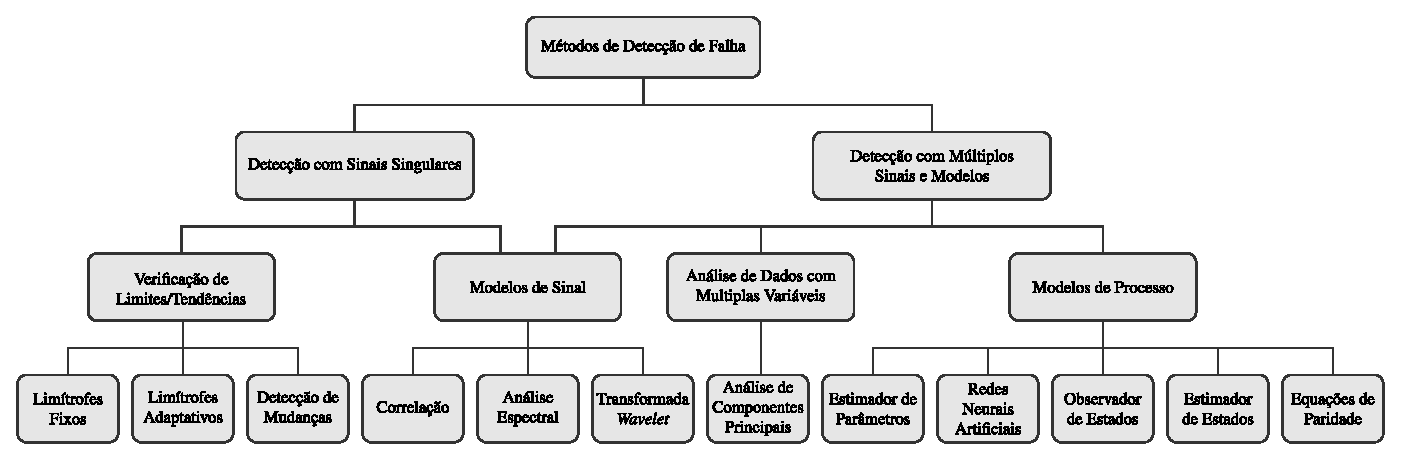
\includegraphics[width=\textwidth]
                        {imgs/introducao/eps/arvore_deteccao}
        \label{fig:arvore_deteccao}
    }
    \subfigure[Métodos de Diagnóstico]
    {
        %\includegraphics[height=0.45\textwidth]
        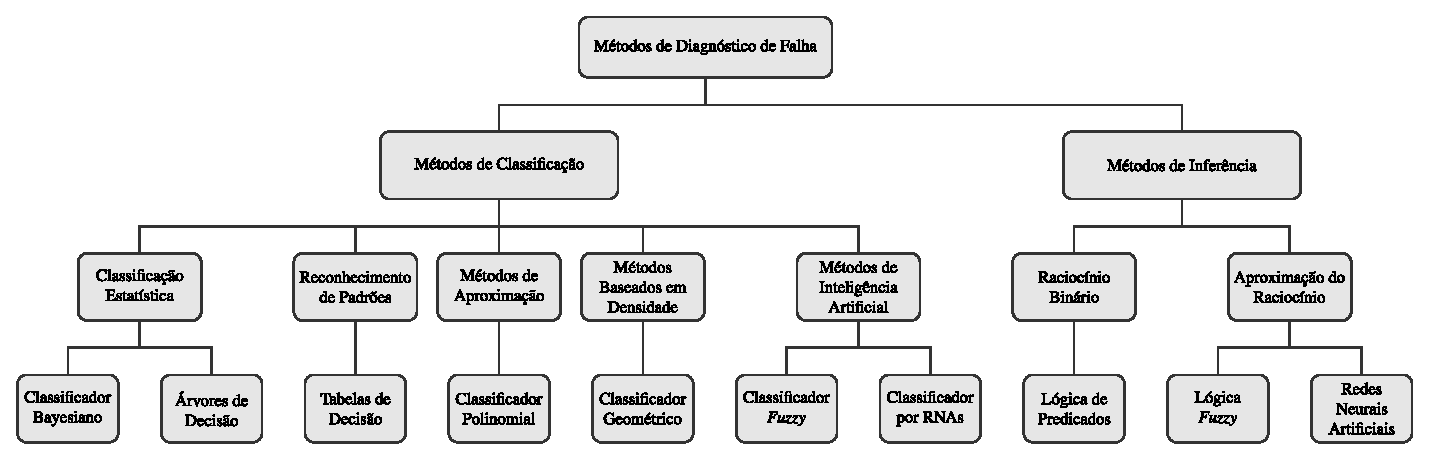
\includegraphics[width=\textwidth]
                        {imgs/introducao/eps/arvore_diagnostico}
        \label{fig:arvore_diagnostico}
    }
    \caption{Métodos de detecção e diagnóstico de falhas.}
    \label{fig:arvores_isermann}
\end{figure}
%\end{landscape}

De maneira complementar, \citeasnoun{venkatasu:2003a} subdividem os algoritmos
de diagnóstico de falhas em três classes, conforme Figs.
\ref{fig:arvore_venkatasu_quant} a \ref{fig:arvore_venkatasu_hist}. Cada uma das
classes é abordada em detalhes nos três artigos que compõem uma revisão
bibliográfica sobre o assunto
\cite{venkatasu:2003a,venkatasu:2003b,venkatasu:2003c}.

\begin{figure}[htb]
\centering
    \subfigure[Algoritmos baseados em Análise Quantitativa]
    {
        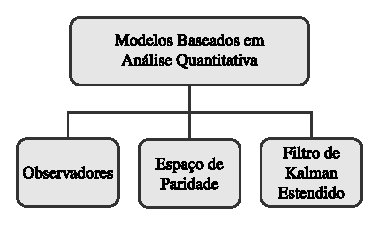
\includegraphics[width=0.3\textwidth]
                        {imgs/introducao/eps/arvore_venkatasu_quant}
        \label{fig:arvore_venkatasu_quant}
    }
    \qquad
    \subfigure[Algoritmos baseados em Análise Qualitativa]
    {
        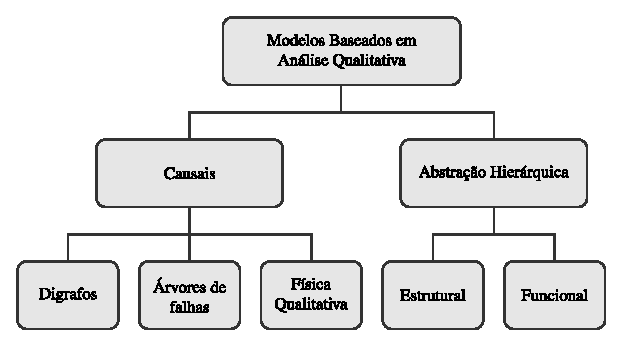
\includegraphics[width=0.51\textwidth]
                        {imgs/introducao/eps/arvore_venkatasu_qual}
    }
    \subfigure[Algoritmos baseados em Histórico do Processo]
    {
        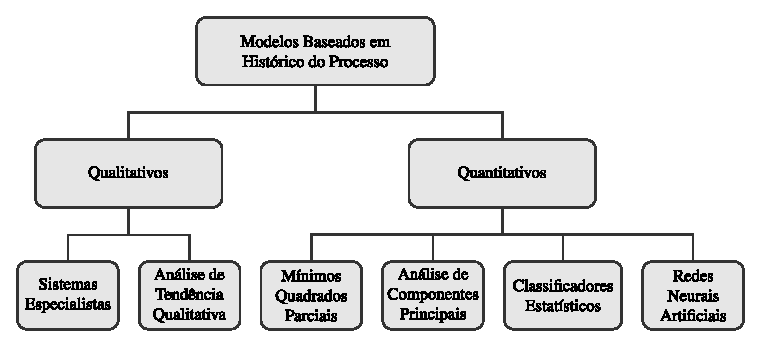
\includegraphics[width=0.6\textwidth]
                        {imgs/introducao/eps/arvore_venkatasu_hist}
        \label{fig:arvore_venkatasu_hist}
    }
    \caption{Classificação dos algoritmos de diagnóstico de falhas.}
    \label{fig:arvore_venkatasu}
\end{figure}

\begin{comment}
\citeasnoun{zhang:2008} tratam ainda sobre diversos tópicos relacionados aos
Sistemas de Controle Tolerante a Falhas (SCTF), outro segmento de pesquisa até
então não mencionado. Mostram para isso que, por razões históricas e por
questões de complexidade, a maioria das pesquisas relacionadas à DDF e às
estratégias de controle reconfiguráveis foram realizadas como duas coisas
separadas. Afirmam também que pouca atenção é dada para a construção de um
sistema ``completo'' que possua essa interação entre um sistema de detecção e
diagnóstico e as estratégias de controle reconfiguráveis.

\Glossary{SCTF}{Sistema de Controle Tolerante à Falhas}

Sendo mais específico, os autores mostram que as técnicas de detecção e
isolamento de falhas foram desenvolvidas como ferramentas de diagnóstico ou de
monitoramento. Como resultado disso, aduzem que os métodos de detecção e
diagnóstico não satisfazem as necessidades das técnicas de controle
reconfigurável, em contraste com o que é exposto na maioria das pesquisas na
área de controle reconfigurável, nas quais assume-se a existência de um sistema
de detecção e diagnóstico perfeito.
\end{comment}

Tendo conhecido alguns dos temas mais abordados ao longo de todos esses anos, o
trabalho a ser aqui apresentado se propõe a desenvolver um sistema que faça uso
de Redes Neurais Artificiais (RNAs) para detectar e diagnosticar as falhas que
venham a ocorrer em um determinado processo dinâmico. O sistema deverá ser capaz
de detectar a presença das falhas, gerando sinais de alarme que notifiquem o
operador e que possam vir a ser pós-processados.

\Glossary{RNA}{Rede Neural Artificial}

Para que isso seja possível, o modelo de estudo de caso será identificado
através de redes neurais, de tal modo que a partir do valor real mensurado e da
inferência realizada pelo modelo identificado, seja gerado um resíduo que, em
conjunto com outros valores, irão compor a entrada da estrutura neural de
detecção e diagnóstico de falhas.

Considerando então os métodos de DDF que fazem uso de RNAs, pode-se destacar uma
série de contribuições. Em \citeasnoun{sreedhar:1995}, por exemplo, é elaborado
um sistema que possui uma rede neural adaptativa capaz de detectar falhas em
sistemas não-lineares. \citeasnoun{vemuri:1998}, por sua vez, propõe um sistema
de detecção de falhas inteligente para manipuladores robóticos. Já em
\citeasnoun{chang:2003} é desenvolvido um sistema que faz uso de RNAs para
detectar curto-circuitos. Em \citeasnoun{talebi:2005} é mostrada uma estrutura
capaz de detectar falhas em sistemas de controle de satélites.
\citeasnoun{jia-li:2010} mostra ainda um sistema capaz de diagnosticar falhas em
sistemas de câmbio automotivo.

Diversas outras contribuições foram feitas através da utilização de técnicas
híbridas. Em \citeasnoun{gao:2000}, por exemplo, é proposto um sistema que
utiliza uma rede neural de Elman, com treinamento assistido por algoritmo
genético para a detecção de falhas em unidades de sistemas de motor.
\citeasnoun{guo:2005} combinam as propriedades das transformadas {\it wavelet}
com RNAs para detecção de falhas em máquinas rotativas Já em
\citeasnoun{tian:2007}, é proposto um sistema Neuro-{\it Fuzzy} para detecção de
falhas em oleodutos. Por fim, \citeasnoun{khaled:2010}, mostra um sistema
composto por um método que combina RNAs com análise de componentes principais,
capaz de identificar e isolar falhas em processos de fabricação.

Assim sendo, os capítulos seguintes do presente texto serão divididos conforme
descrição a seguir. O Capítulo \ref{cap:rnas} irá abordar os conceitos sobre as
RNAs, mostrando suas arquiteturas e modelos de identificação que serão
utilizados no trabalho. Em seguida, o Capítulo \ref{cap:detec_diag} irá tratar
sobre as terminologias utilizadas e os métodos de detecção e diagnóstico de
falhas. Já o Capítulo \ref{cap:sistema}, irá conter a descrição detalhada do
processo escolhido como estudo de caso e mostrará algumas possibilidades de como
o sistema final poderá ser composto. Por fim, nos dois últimos capítulos, serão
apresentados e discutidos os resultados obtidos para cada uma das estruturas
idealizadas no Capítulo \ref{cap:sistema}, encerrando com uma breve conclusão e
mostrando as possibilidades de trabalhos futuros.

\mychapter{Aspectos de projeto}
\label{cap:aspectos}

Com a demanda cada vez mais crescente com relação a eficiência, a qualidade dos
produtos e integração dos processos no setor industrial, aliada aos altos custos
envolvidos e as mais diversas necessidades de segurança, torna-se claro a
importância dos sistemas de supervisão e dos sistemas de DDF
\cite{isermann:2006}.

Atualmente, devido ao nível de complexidade envolvido em um processo industrial,
os sistemas de supervisão e proteção exigem as mais avançadas técnicas
oferecidas pela engenharia moderna e ainda assim demandam um esforço contínuo
por parte dos pesquisadores e engenheiros, para que sejam desenvolvidas novas
tecnologias que venham a suprir essa necessidade \cite{silva:2008}.

Considerando tais aspectos, este capítulo mostrará os conceitos relacionados ao
desenvolvimento de um sistema de DDF que fará uso de RNAs. Inicialmente, serão
mostradas as principais terminologias utilizadas na área. Em seguida a atenção
será voltada para as RNAs e suas estruturas de identificação. Por fim, será
mostrado rapidamente como o sistema será estruturado para que sejam feitas as
simulações computacionais.

% ------------------------------------------------------------------------------
\section{Conceitos e terminologias}\label{sec:propriedades}
Segundo \citeasnoun{kaanich:2002}, os sistemas computacionais podem ser
caracterizados por cinco propriedades fundamentais: funcionalidade, usabilidade,
desempenho, custo e {\it dependabilidade}. Para \citeasnoun{laprie:1992}, o
termo {\it dependabilidade}, que nada mais é do que a tradução literal do termo
inglês {\it dependability}, está relacionado com a capacidade de um sistema
prestar um serviço que possa ser, justificadamente, confiável. O serviço
prestado se refere ao comportamento do sistema percebido por seus usuários, os
quais também serão sistemas (máquinas físicas ou seres humanos), que interagem
com o anterior.

De acordo com \citeasnoun{laprie:1994}, dependendo das aplicações envolvidas, o
termo dependabilidade pode ainda ser visto de acordo com suas diferentes, mas
complementares, propriedades:

\begin{itemize}
    \item {\bf Disponibilidade:} Prontidão para o uso;
    \item {\bf Confiabilidade:} Continuidade do serviço;
    \item \textbf{Proteção (\textit{safety}):} Não ocorrência de consequências
          catastróficas para o meio;
    \item {\bf Confidencialidade:} Não ocorrência da divulgação não-autorizada
          da informação;
    \item {\bf Integridade:} Não ocorrência de alterações indevidas da
          informação;
    \item {\bf Manutenção:} Aptidão para sofrer reparos e evolução.
\end{itemize}

A associação da integridade com a disponibilidade e a confidencialidade leva à
\textbf{Segurança (\textit{security})}.

Apesar do termo dependabilidade ser utilizado na maioria das vezes dessa forma,
o dicionário Michaelis, traduz tal termo como {\it confiabilidade} ou {\it
garantia de funcionamento}. Assim sendo, daqui para frente, utilizar-se-á a
palavra {\it confiável}, ou suas variações linguísticas, para se referir ao
termo {\it dependable}. Quando for desejado fazer referência a propriedade da
confiabilidade de um sistema, tal intenção será claramente especificada pelo
texto.

% ------------------------------------------------------------------------------
\section{Sistemática da dependabilidade}
\citeasnoun{avizienis:2000} e \citeasnoun{kaanich:2002} mostram que para se
desenvolver um Sistema Computacional Confiável (SCC, do inglês {\it Dependable
Computing System -- DCS}), faz-se uso de diferentes técnicas, tais como as
técnicas de: {\bf prevenção}, {\bf tolerância}, {\bf supressão} e {\bf previsão}
de falhas.

O estudo sobre a {\it prevenção} de falhas envolve a seleção de metologias de
projeto e de tecnologias adequadas para a escolha e a aplicação dos componentes
no sistema, ou seja, busca não introduzir ou evitar que aconteçam falhas. A {\it
tolerância} a falhas está mais relacionada com a continuidade da prestação do
serviço quando uma falha vier a ocorrer. Algumas das técnicas mais conhecidas
são: mascaramento de falhas, redundância de dispositivos/sistemas e a
detecção/recuperação de falhas. A {\it supressão} das falhas procura minimizar
as consequências relativas à presença de uma falha através de mecanismos de
verificação, diagnóstico e correção. A {\it previsão} de falhas está relacionada
com a estimativa que pode ser feita sobre a presença, a criação e a consequência
que as falhas venham a causar no sistema. Para isso, faz uso de critérios
avaliativos, técnicas de injeção de falhas e testes de resistência.

Além dessas técnicas, é válido também fazer referência aos termos {\bf avaria},
{\bf erro} e {\bf falha}, conceitualmente abordados de diferentes maneiras por
vários autores. Os conceitos relativos a essa nomenclatura serão melhor
explicados na seção \ref{sec:avaria_erro_falha}.

\begin{comment}
\begin{itemize}
    \item {\bf Técnicas de prevenção:} Como prevenir a ocorrência ou a introdução de
          falhas;
    \item {\bf Técnicas de tolerância:} Como oferecer um serviço ``correto'' na
          presença de falhas;
    \item {\bf Técnicas de supressão:} Como reduzir o número ou atenuar a
          gravidade das falhas;
    \item {\bf Técnicas de previsão:} Como estimar o número atual, a incidência
          futura e as consequências das prováveis falhas.
\end{itemize}
\end{comment}

A partir dessas informações, \citeasnoun{avizienis:2000} separa os termos acima
relacionados em três grupos: os atributos (propriedades), as ameaças e os meios
pelos quais a dependabilidade é atingida. Tal divisão pode ser observada na Fig.
\ref{fig:div_avizienis}.

\begin{figure}[htb]
\centering
\footnotesize
\[
\text{Dependabilidade}
\left\{
\begin{array}{l}
\text{Atributos}
    \left\{
    \begin{array}{l}
        \text{Disponibilidade}\\
        \text{Confiabilidade}\\
        \text{Proteção}\\
        \text{Confidencialidade}\\
        \text{Integridade}\\
        \text{Manutenção}\\
        \text{Segurança}
    \end{array}
    \right.
\\
\\
\text{Ameaças}
    \left\{
    \begin{array}{l}
        \text{Avaria}\\
        \text{Erro}\\
        \text{Falha}
    \end{array}
    \right.
\\
\\
\text{Meios}
    \left\{
    \begin{array}{l}
        \text{Prevenção}\\
        \text{Tolerância}\\
        \text{Supressão}\\
        \text{Previsão}
    \end{array}
    \right.
\end{array}
\right.
\]
\caption{Classificação sistemática da dependabilidade.}
\label{fig:div_avizienis}
\end{figure}

O primeiro grupo, cujos elementos foram brevemente explicados na seção
\ref{sec:propriedades}, permite expressar as propriedades esperadas e analisar a
qualidade de um sistema confiável. Já o segundo grupo traz os termos utilizados
para expressar características indesejadas -- mas em princípio não inesperadas
-- que causa ou fazem com que um sistema passe a ser não-confiável. Por fim, o
terceiro grupo exibe os meios ou as técnicas pelas quais torna-se possível
oferecer um serviço confiável.

% ------------------------------------------------------------------------------
\section{Avarias, erros e falhas}\label{sec:avaria_erro_falha}
Em um processo real, todos os recursos utilizados, sejam físicos ou
implementados em {\it software}, estão sujeitos a interrupções ou a
comprometimentos operacionais.

Em sistemas críticos, tais como as aeronaves ou as usinas nucleares, essas
situações fazem com que pequenos ``deslizes operacionais'' venham a trazer
grandes e indesejáveis consequências. Dentre diversos outros exemplos, pode-se
destacar o acidente do {\it Airbus 320} da TAM em 2007, que não conseguiu parar
ao aterrissar no aeroporto de Congonhas, São Paulo, no qual morreram 199 pessoas
(12 em solo e 187 no avião) e o desastre da usina nuclear de Chernobil, que
liberou cerca de 400 vezes mais contaminação do que a bomba nuclear que foi
lançada em de Hiroshima.

Esses exemplos fazem-nos refletir sobre como os sistemas de controle podem
evoluir para evitar que catástrofes ainda maiores venham a ocorrer. Ou seja,
como as propriedades de um sistema de controle confiável poderão ser mantidas
mesmo na presença de avarias, erros e falhas no processo.

Segundo \citeasnoun{nelio:2002}, apesar do termo falha ser utilizado, em muitos
dos casos, como um termo vago, abrangendo também o significado de avarias e
erros, existe uma diferença entre esses conceitos que deve ser destacada.

O termo {\bf avaria} ({\it failure}) deve ser utilizado para indicar que houve
um desvio do comportamento no sistema, o que o torna incapaz de fornecer o
serviço para o qual foi designado. Um {\bf erro} ({\it error}), entretanto, está
relacionado com estado do sistema e pode levar a uma avaria. De maneira
resumida, se há um erro no estado do sistema, então existe uma sequência de
ações que podem ser executadas e que levarão a avarias, a não ser que medidas de
correção venham a ser tomadas. Por fim, mas não menos importante, o termo {\bf
falha} ({\it fault}) é a causa de um erro e está associado à noção de defeitos.
Normalmente, diz-se que falha pode ser definida como sendo um defeito que possui
o potencial de gerar erros \cite{nelio:2002,weber:2002}.

Alguns autores nacionais costumam traduzir os termos {\it failure} como falha e
{\it fault} como falta. Entretanto, costuma-se falar em sistemas de controle
tolerante a ``falhas'' e não em sistemas de controle tolerantes a ``faltas''.
Observa-se então a necessidade de um maior cuidado com relação a utilização
dessas palavras, pois as avarias ({\it failures}) não podem ser toleradas.

\begin{comment}
Por esse motivo, ao longo do texto, quando for necessário se referir ao termo
{\it failure}, será utilizada a palavra avaria. Já o termo falha será utilizado
de maneira mais abrangente, envolvendo os conceitos de erro e de falha
explicados anteriormente.
\end{comment}

Como em muitos dos casos os sistemas são compostos de subsistemas, é comum se
observar que uma falha leva a um erro que por sua vez pode levar a uma avaria,
que gera novas falhas e dá início a uma reação em cadeia, tal como a Fig.
\ref{fig:reacao_cadeia}. Contudo, nem sempre uma falha conduz a um erro, assim
como nem sempre um erro conduz a uma avaria, mas todos os erros resultam de
falhas e todas as avarias resultam de erros.

\begin{figure}[htb]
\centering
\[
\ldots
\quad\Longrightarrow\quad
\text{Falha} 
\quad\longrightarrow\quad
\text{Erro}
\quad\longrightarrow\quad
\text{Avaria}
\quad\Longrightarrow\quad
\text{Falha}
\quad\longrightarrow\quad
\ldots
\]
    \caption{Reação em cadeia das falhas, erros e avarias.}
    \label{fig:reacao_cadeia}
\end{figure}

Uma outra maneira de visualizar a diferença existente entre cada um desses
termos pode ser observada na Fig. \ref{fig:mapa_conceitos}.

\begin{figure}[htb]
\centering
    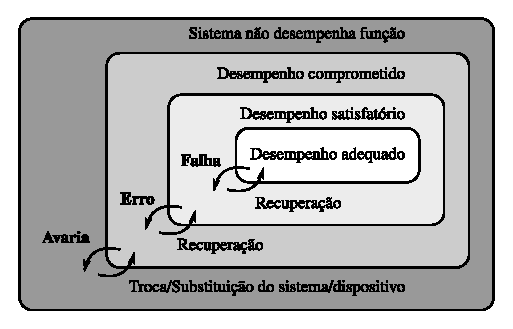
\includegraphics[width=0.5\textwidth]{imgs/aspectos/eps/mapa_conceitos}
    \caption{Mapa de conceitos relacionados a avarias, erros e falhas em um
             sistema.}
    \label{fig:mapa_conceitos}
\end{figure}

\citeasnoun{weber:2002} afirma ainda que as falhas são inevitáveis, uma vez que
os componentes físicos do sistema envelhecem e estão sempre sujeitos as
interferências externas, ambientais ou humanas. Mostra também que, assim como os
sistemas físicos, os {\it softwares} também são vítimas, pois estão a mercê da
alta complexidade dos processos e da fragilidade humana em trabalhar com grande
volume de detalhes de especificação/operação.

% ------------------------------------------------------------------------------
\subsection{Tipos de falhas}

\begin{comment}
\citeasnoun{laprie:1994} mostra que existem cinco classes elementares para as
falhas, conforme Fig. \ref{fig:class_laprie}.

\begin{figure}[htb]
\centering
\footnotesize
\[
\text{Falha}
\left\{
\begin{array}{l}
\text{Causas fenomenológicas}
    \left\{
    \begin{array}{l}
        \text{Falhas físicas}\\
        \text{Falhas humanas}
    \end{array}
    \right.
\\
\\
\text{Natureza}
    \left\{
    \begin{array}{l}
        \text{Falhas acidentais}\\
        \text{Falhas intencionais, não-maliciosas}\\
        \text{Falhas intencionais, maliciosas}
    \end{array}
    \right.
\\
\\
\text{Criação/Ocorrência}
    \left\{
    \begin{array}{l}
        \text{Falhas de desenvolvimento}\\
        \text{Falhas operacionais}
    \end{array}
    \right.
\\
\\
\text{Limitações do sistema}
    \left\{
    \begin{array}{l}
        \text{Falhas internas}\\
        \text{Falhas externas}
    \end{array}
    \right.
\\
\\
\text{Persistência}
    \left\{
    \begin{array}{l}
        \text{Falhas permanentes}\\
        \text{Falhas temporárias}
    \end{array}
    \right.
\end{array}
\right.
\]
    \caption{As cinco classes elementares das falhas.}
    \label{fig:class_laprie}
\end{figure}

\end{comment}

De acordo com \citeasnoun{silva:2008}, as falhas em um processo industrial podem
ser classificadas em relação a vários aspectos. Em se tratando da classificação
quanto ao tempo, as falhas podem ser abruptas, incipientes ou intermitentes, tal
como mostra a Fig. \ref{fig:tipos_falha}.

\begin{figure}[H]
\centering
    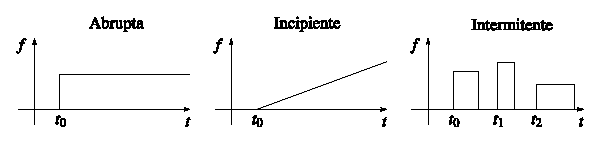
\includegraphics[width=0.75\textwidth]{imgs/aspectos/eps/tipos_falha}
    \caption{Características temporais das falhas quanto a sua persistência.}
    \label{fig:tipos_falha}
\end{figure}

\begin{comment}
De acordo com essa classificação, percebe-se que não existirá um sistema
que venha a falhar somente uma vez. Por mais que as falhas demorem a acontecer,
elas são inevitáveis.
\end{comment}

As {\it falhas abruptas} surgem repentinamente, podendo ser decorrentes de
imprevistos ou até mesmo de acidentes. Essas falhas mudam o comportamento do
processo rapidamente, exigindo contra-ações velozes e eficazes que possam
minimizar as consequências do ocorrido.

As {\it falhas incipientes} iniciam a partir de pequenos desvios comportamentais
do sistema, podendo ser mascaradas pelos controladores.  Muitas vezes essas
falhas acabam passando despercebidas pelos operadores ou até mesmo pelos
sistemas de detecção e diagnóstico de falhas.

As {\it falhas intermitentes} são aquelas que ocorrem durante um certo período
de tempo e, em seguida, desaparecem, voltando a aparecer após um novo intervalo.
Podem ser causadas por alguma perturbação periódica ou por alguma situação que
se repita ciclicamente.

Considerando a localização das falhas, estas podem ocorrer nos sensores, nos
atuadores ou na estrutura do sistema \cite{silva:2008}. As {\it falhas nos
sensores} podem ser observadas através de variações específicas nas medições, as
quais podem ser descaracterizadas como variações válidas do sistema. As {\it
falhas nos atuadores} podem ser vistas como qualquer mau funcionamento do
equipamento que atua no sistema. As {\it falhas na estrutura}, ou {\it falhas
estruturais}, ocorrem quando alguma alteração do sistema muda, de alguma forma,
a relação original de entrada e saída do processo ou quando ocorre algum
problema com algum dos dispositivos, desde que não sejam sensores ou atuadores,
como por exemplo, os transmissores de sinal.

Considerando então um processo genérico, pode-se citar como exemplos de falhas
aquelas exibidas pela Tab. \ref{tab:falhas}.

\begin{table}[htb]
\centering
\caption{Exemplos de falhas para um processo genérico.}
\label{tab:falhas}
\vspace{0.25cm}
\begin{tabular}{|c|c|c|}
\hline
{\bf Sensores} & {\bf Atuadores} & {\bf Estrutura}\\
\hline
\hline
Erro de leitura & Erro de escrita & Erro de transmissão\\
\hline
Descalibramento & Erro de leitura & Perda de comunicação\\
\hline
Sensibilidade à ruído & Sensibilidade à ruído & Sensibilidade a ruído
(transmissor)\\
\hline
Queima & Queima & Queima (transmissor)\\
\hline
- & Atraso de transporte & Atraso de propagação de sinais\\
\hline
\end{tabular}
\end{table}

Maiores detalhes sobre as propriedades e a classificação das falhas podem ser
encontradas em \citeasnoun{laprie:1992}, \citeasnoun{laprie:1994},
\citeasnoun{weber:2002} e \citeasnoun{isermann:2006}.

% ------------------------------------------------------------------------------
%\section{Os meios para se atingir a dependabilidade}
%\label{sec:tecnicas}

% ------------------------------------------------------------------------------
\section{Detecção e diagnóstico de falhas}
Segundo \citeasnoun{chiang:2001}, detectar, diagnosticar e ``remover'' uma falha
é uma das formas de se garantir que as operações de um processo satisfaçam as
especificações de desempenho. Essas ações estão associadas com a noção de
supervisão e monitoramento de processos.

Para eles, supervisionar e monitorar determinado processo tem por objetivo
garantir o sucesso das operações planejadas e reconhecer as anomalias
comportamentais. A informação a ser disponibilizada por um sistema de
monitoramento não deve, tão somente, informar ao operador do sistema sobre o que
está acontecendo, mas auxiliá-lo a tomar medidas corretivas com o intuito de
sanar o problema. Como resultado disso, o tempo em que o sistema estará
inoperante será reduzido, a proteção do sistema aumentará e os custos
relacionados diminuirão.

Uma vez que os processos industrias estão se tornando cada vez mais integrados e
complexos, a ocorrência de falhas também passa a ser um fator de complicação. As
falhas que antes poderiam ser detectadas facilmente por medições diretas de
determinada variável passam a depender de um conjunto de variáveis que atuam
simultaneamente. Além disso, se uma falha é detectada em um determinado ponto de
um sistema sistema, a causa do problema pode estar próxima ou distante,
dependendo do grau de complexidade envolvido. Como exemplo, uma simples falha em
uma aeronave pode causar indicações de falha em diversos subsistemas de
segurança \cite{vach:2006}.

Para \citeasnoun{chiang:2001}, existem quatro fases envolvidos no monitoramento
de processos: {\bf detecção}, {\bf isolamento}, {\bf diagnóstico} e {\bf
recuperação} de falhas, conforme mostrado pela Fig.
\ref{fig:fases_monitoramento}.

\begin{figure}[htb]
\centering
    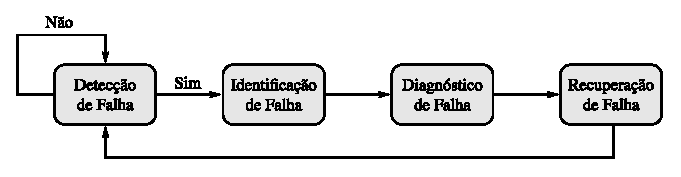
\includegraphics[width=0.65\textwidth]{imgs/aspectos/eps/fases_monitoramento}
    \caption{Fases envolvidas no monitoramento de processos.}
    \label{fig:fases_monitoramento}
\end{figure}

A {\it detecção da falha} consiste em determinar se ocorreu ou não uma falha. A
detecção antecipada ou precoce pode fornecer informações valiosas quanto aos
problemas que venham a surgir. Através de ações apropriadas, pode-se evitar
perturbações graves ao processo.

A {\it identificação da falha} tem por objetivo identificar as variáveis mais
importantes para que se realize um diagnóstico apropriado. Para isso, essa fase
procura concentrar as atenções do operador nos subsistemas mais pertinentes à
falha, de tal modo que o efeito desta possa ser eliminado de maneira mais
eficiente.

A fase de {\it diagnóstico da falha} determina que falha ocorreu. De acordo com
\citeasnoun{isermann:2004}, essa fase deverá indicar o maior número de detalhes
possíveis a respeito da falha, tais como a intensidade, a localização e o
momento em que a falha foi detectada. Essa fase é considerada essencial para uma
contra-ação ou eliminação da falha.

A fase de {\it recuperação da falha}, também conhecida como fase de {\it
intervenção}, tem por objetivo remover o efeito da falha para com o sistema,
dando início a um novo ciclo de detecção e diagnóstico.

Apesar de estarem explicitamente colocados como uma sequência de ações, nem
sempre todas as fases são estritamente necessárias necessárias
\cite{chiang:2001}. 

Para \citeasnoun{venkatasu:2003a}, a automatização das formas de detecção e
diagnóstico compõe o primeiro passo de um sistema de gestão de eventos anormais
Ao longo de vários anos, muitas soluções vem sendo desenvolvidas e um grande
número de técnicas já foram utilizadas. Exemplos dessas técnicas são as árvores
de falhas, os digrafos, as abordagens analíticas, os sistemas especialistas e as
RNAs.

\fussy
Do ponto de vista de modelagem, existem métodos que exigem grande precisão com
relação ao modelo de processo, outros que exigem modelos semi-quantitativos ou
ainda modelos qualitativos. Por outro lado, existem métodos que não necessitam
de nenhuma informação do modelo, utilizando somente informações do histórico do
processo \cite{venkatasu:2003a}.
\sloppy

Conforme mostrado no Capítulo \ref{cap:introducao}, a classificação dos métodos
de DDF pode variar de autor para autor
\cite{venkatasu:2003a,angeli:2004,zhang:2008,isermann:2006}. A abordagem aqui
escolhida irá considerar a classificação adotada em \citeasnoun{isermann:2006},
até então considerada a mais intuitiva.

% ------------------------------------------------------------------------------
\section{Métodos de detecção}
Nas seções seguintes será feita uma breve análise dos métodos de detecção de
falhas abordados em \citeasnoun{isermann:2006}. Vale salientar que existem, na
literatura, vários outros métodos de detecção de falhas. Deseja-se aqui trazer
alguns exemplos.

% ------------------------------------------------------------------------------
\subsection{Detecção de falhas com verificação de limites}
Considerado como um dos métodos mais simples e intuitivos, a detecção de falhas
com verificação de limites baseia-se na medição direta de uma determinada
variável e a comparação de seu valor absoluto ou de sua tendência com um
limítrofe previamente especificado.

A verificação de valores absolutos, estabelece que dois limiares ou limítrofes
fixos são estabelecidos: $Y_{max}$ e $Y_{min}$. O funcionamento normal do
sistema consiste em verificar se a variável $Y$ está ou não contida nesse
intervalo:

\begin{equation}
Y_{min} < Y < Y_{max}
\end{equation}

Essa abordagem considera que o processo está funcionando normalmente quando a
variável monitorada encontra-se dentro de uma zona de tolerância. Quando a
variável monitorada excede um dos limiares estabelecidos, deduz-se que haverá
uma falha em algum ponto do processo.

Por mais simples que pareça, este método é aplicado na maioria dos sistemas de
automação, tais como: verificação da pressão mínima em oleodutos, da temperatura
máxima em sistemas de refrigeração de motores, a pressão mínima de circulação de
gás em refrigeradores.

Uma outra abordagem utiliza a verificação de tendência da variável medida. Um
exemplo simples faz uso da primeira derivada da variável $\dot{Y} = dY(t)/dt$ e
verifica se esta tendência está ou não dentro de uma faixa pré-estabelecida:

\begin{equation}
\dot{Y}_{min} < \dot{Y} < \dot{Y}_{max}
\end{equation}

Exemplos dessas duas abordagens podem ser observados na Fig.
\ref{fig:detec_ver_lim}.

\begin{figure}[htb]
\centering
    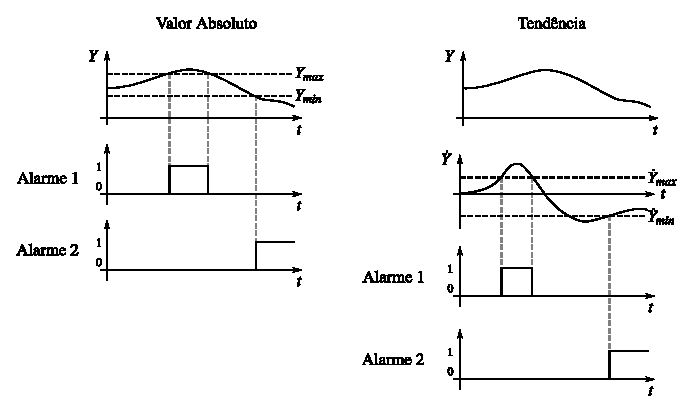
\includegraphics[width=0.85\textwidth]{imgs/aspectos/eps/detec_ver_lim}
    \caption{Exemplo de detecção com verificação de limites.}
    \label{fig:detec_ver_lim}
\end{figure}

% ------------------------------------------------------------------------------
\subsection{Detecção de falhas com modelos de sinais}
Diversos sinais medidos em um processo apresentam oscilações de natureza
harmônica ou estocástica. Se as mudanças nesse sinal estiverem relacionadas com
as falhas nos sensores, atuadores ou ainda com as falhas estruturais, uma
maneira de se detectar essas falhas é o de se utilizar métodos de detecção
baseados em modelos de sinais.

Em se tratando de vibrações em máquinas, por exemplo, a medição da posição,
da velocidade ou da aceleração permite que muitos tipos de falhas sejam
detectadas.

% ------------------------------------------------------------------------------
\subsection{Detecção de falhas com observadores e estimadores de estado}

% ------------------------------------------------------------------------------
\subsection{Detecção de falhas com métodos de identificação}

% ------------------------------------------------------------------------------
\section{Métodos de diagnóstico}

% ------------------------------------------------------------------------------
\subsection{diagnóstico de falhas com métodos de classificação}

% ------------------------------------------------------------------------------
\subsection{diagnóstico de falhas com métodos de inferência}

% ------------------------------------------------------------------------------
\section{Detecção e diagnóstico de falhas com RNAs}

Com a introdução das novas tecnologias de medição e o consequente aumento do
número de instrumentos nos processos industrias, as informações e os dados
disponíveis da operação do sistema passam a ser essenciais para as atividades de
supervisão e controle. Como exemplo, diversas estratégias de detecção e
diagnóstico de falhas fazem uso do histórico do processo ........ dentre essas
estratégias... RNAs

% ------------------------------------------------------------------------------
\section{Redes neurais artificiais}

% ------------------------------------------------------------------------------
\subsection{Tipos de RNAs para identificação}

% ------------------------------------------------------------------------------
\subsection{Tipos de RNAs para detecção}

% ------------------------------------------------------------------------------
\section{Simulações computacionais}

% ------------------------------------------------------------------------------
\subsection{Método de Runge-Kutta de 4\textordfeminine ordem}

\mychapter{Sistema proposto}
\label{cap:sistema}
Existem diversos métodos consolidados para detecção e isolamento de falhas,
sendo alguns deles baseados em redundância física de componentes de hardware,
como sensores, atuadores e controladores. Entretanto, a duplicação de
componentes de hardware nem sempre é possível, uma vez que os custos
relacionados com a adição de novos componentes componente podem elevar o
orçamento do processo demasiadamente.

Devido a esse elevado custo, existe uma fronteira clara e inerente à aplicação
de técnicas de tolerância a falhas. A escolha adequada dos dispositivos físicos
e dos {\it softwares} devem então levar em consideração as exigências
específicas de cada sistema de maneira individual, de tal maneira que se possa
contornar o custo associado ao emprego dessas técnicas \cite{weber:2002}.

Assim sendo, a primeira parte do capítulo descreverá em detalhes o modelo de
estudo de caso escolhido para ser simulado, mostrando suas características e
limitações. Em seguida a atenção será voltada para as estruturas neurais de
identificação do modelo e de detecção das falhas, mostrando ao final como serão
realizadas as simulações.

% ------------------------------------------------------------------------------
\section{Estudo de caso}
Ao final do Cap. \ref{cap:introducao}, após ter-se comentado sobre a utilização
das RNAs em sistemas de DDF, propôs-se que será desenvolvido um sistema para
realizar a detecçao e o diagnóstico de falhas em um processo dinâmico. Para que
isso seja possível serão utilizadas estruturas neurais que farão uso de
determinados valores obtidos a partir das medições realizadas no processo.

O processo em questão, ao qual se refere o parágrafo anterior, é formado por um
sistema de tanques acoplados desenvolvidos pela Quanser\reg, representado
esquematicamente na Fig. \ref{fig:tanques}.

\begin{figure}[htb]
\centering
    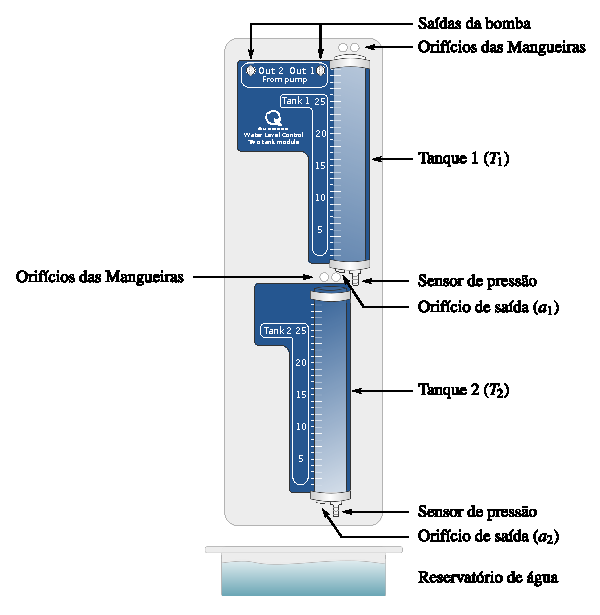
\includegraphics[width=0.7\textwidth]{imgs/sistema/eps/tanques}
    \caption{Sistema de tanques acoplados da Quanser\reg.}
    \label{fig:tanques}
\end{figure}

O sistema original consiste de uma bomba de água de corrente contínua e dois
tanques acoplados. A alimentação de água pela bomba se dá de forma vertical
através de dois orifícios com conectores normalmente fechados, de diferentes
diâmetros, denominados {\it Out 1} e {\it Out 2}. Para facilitar o entendimento
e evitar confusões com relação aos orifícios de saída dos tanques ($a_1$ e
$a_2$), esses orifícios serão tratados como orifícios de entrada.

\Glossary{$a_i$}{Orifício de saída $i$}

Os tanques ($T_1$ e $T_2$) são montados na parte frontal do suporte de base e
posicionados de tal forma que a água flui do tanque superior ($T_1$) para o
tanque inferior ($T_2$) através do orifício $a_1$, e do tanque inferior para o
reservatório através do orifício $a_2$. As vazões de saída dos tanques variam de
acordo com a mudança desses orifícios, disponibilizados em três diâmetros
diferentes pelo fabricante.

\Glossary{$T_1$}{Tanque superior}
\Glossary{$T_2$}{Tanque inferior}

Além dos diferentes orifícios de saída, o fabricante também disponibiliza um
conjunto de mangueiras, tornando possível a utilização dos dois orifícios de
entrada, bombeando água para os dois tanques simultaneamente. As dimensões de
cada um dos orifícios e os demais parâmetros do sistema podem ser visualizadas
na Tab. \ref{tab:dimensoes}.

\begin{table}[!htb]
\centering
\caption{Dimensões e parâmetros do sistema de tanques.}
\label{tab:dimensoes}
\vspace{0.25cm}
\begin{tabular}{|l|c|c|c|}
\hline
{\bf Nome} & {\bf Símbolo} & {\bf Valor} & {\bf Unidade}\\
\hline
\hline
\multicolumn{4}{|l|}{{\bf Bomba}}\\
\hline
Constante de fluxo & $K_m$ & 4,6 & (cm${}^3$/s)/V\\
\hline
Limites de Tensão & $V_{p_{\text{\tiny MAX/MIN}}}$ & $\pm 15$ & Volts\\
\hline
Orifício de entrada 1 & {\it Out 1} & 0,635 & cm\\
\hline
Orifício de entrada 2 & {\it Out 2} & 0,4763 & cm\\
\hline
\multicolumn{4}{|l|}{{\bf Tanque 1/Tanque 2}}\\
\hline
Altura & $H_1$/$H_2$ & 30 & cm\\
\hline
Diâmetro interno & -- & 4,445 & cm\\
\hline
Área de secção transversal & $A_1$/$A_2$ & 15,517916547 & cm${}^2$\\
\hline
Sensibilidade do sensor & -- & 5 & cm/V \\
\hline
\multicolumn{4}{|l|}{{\bf Orifícios de saída -- Diâmetros}}\\
\hline
Orifício pequeno & $a_{i_{\text{\tiny PEQ}}}$ & 0,3175 & cm\\
\hline
Orifício médio & $a_{i_{\text{\tiny MED}}}$ & 0,47625 & cm\\
\hline
Orifício grande & $a_{i_{\text{\tiny GDE}}}$ & 0,555625 & cm\\
\hline
\multicolumn{4}{|l|}{{\bf Orifícios de saída -- Áreas}}\\
\hline
Orifício pequeno & $a_{i_{\text{\tiny PEQ}}}$ & 0,079173044 & cm${}^2$\\
\hline
Orifício médio & $a_{i_{\text{\tiny MED}}}$ & 0,178139348 & cm${}^2$\\
\hline
Orifício grande & $a_{i_{\text{\tiny GDE}}}$ & 0,242467446 & cm${}^2$\\
\hline
\multicolumn{4}{|l|}{{\bf Sensores}}\\
\hline
{\it Range} de pressão & -- & 0 - 1 & PSI\\
\hline
{\it Range} de nível & -- & 0 - 30 & cm\\
\hline
Constante de sensibilidade & $K_s$ & $6,25\times$ & cm/V\\
\hline
\end{tabular}
\end{table}

Dentre as várias combinações possíveis obtidas a partir da mudança dos orifícios
de entrada e saída, as três configurações sugeridas pelo manual do fabricante
encontram-se representadas na Fig. \ref{fig:config_fab}. Cada uma dessas
configurações modifica a dinâmica do processo, permitindo que sejam projetados e
analisados diferentes tipos de controladores.

\begin{figure}[!htb]
\centering
\subfigure[Configuração 1.]
{
    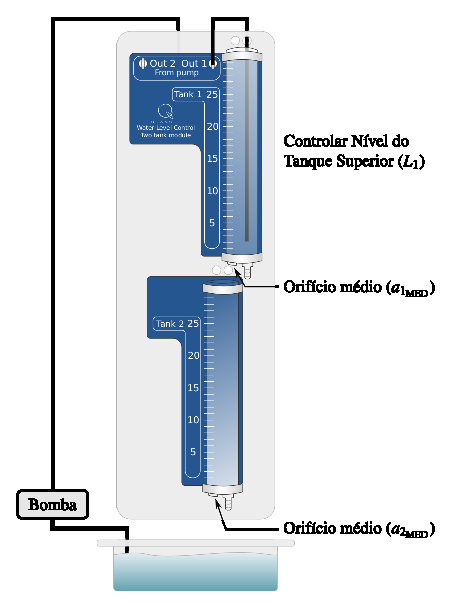
\includegraphics[width=0.31\textwidth]{imgs/sistema/eps/config_fab_1}
    \label{fig:config_fab_1}
}
\subfigure[Configuração 2.]
{
    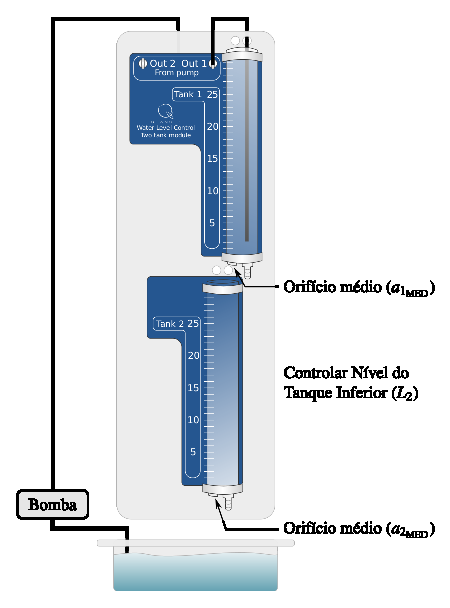
\includegraphics[width=0.31\textwidth]{imgs/sistema/eps/config_fab_2}
    \label{fig:config_fab_2}
}
\subfigure[Configuração 3.]
{
    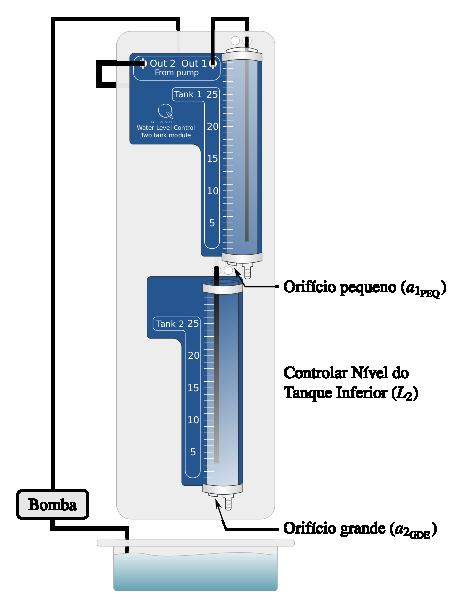
\includegraphics[width=0.31\textwidth]{imgs/sistema/eps/config_fab_3}
    \label{fig:config_fab_3}
}
\caption{Configurações sugeridas pelo fabricante.}
\label{fig:config_fab}
\end{figure}

Na primeira configuração deseja-se controlar o nível de $T_1$ ($L_1$) através de
uma alimentação direta, não fazendo uso do segundo tanque. Na segunda
configuração deseja-se controlar o nível de $T_2$ ($L_2$) a partir de uma
alimentação indireta em $T_1$. Assim, $T_2$ é alimentado a partir da água que
escoa de $T_1$ pelo orifício $a_1$. Por fim, na terceira configuração, deseja-se
controlar o nível de $T_2$ a partir da alimentação indireta de $T_1$ e da
alimentação direta de $T_2$. Para isso, faz-se uso dos dois orifícios de
entrada.

\Glossary{$L_1$}{Nível do tanque superior}
\Glossary{$L_2$}{Nível do tanque inferior}

Em todos os casos pode-se perceber que o sistema se comporta como um sistema de
uma única entrada, que é a tensão de alimentação da bomba, e uma única saída
({\it Single Input and Single Output} -- SISO), que pode ser $L_1$ ou $L_2$,
dependendo da configuração.

\Glossary{SISO}{{\it Single Input and Single Output}}

Além dessas observações, deve-se destacar ainda que a planta em questão se trata
de um modelo desenvolvido para fins acadêmicos e que, por esse motivo, existem
alguns restrições quanto as interfaces e aos padrões de comunicação.

% ------------------------------------------------------------------------------
\subsection{Modelo matemático}

Como os dois tanques possuem mesma área de secção transversal ($A_1 = A_2$), a
dinâmica dos dois tanques será semelhante. Entretanto, encontrar um modelo
matemático que descreva adequadamente a dinâmica desses tanques não é algo tão
simples, visto que as equações gerais de movimento e energia que descrevem o
escoamento de fluidos são bastante complicadas \cite{dorf:2009}.

Assim sendo, é preciso que sejam feitas algumas hipóteses fundamentais.
Admite-se que a água no tanque é incompressível e que o escoamento é
não-viscoso, não-rotacional e regular. Cada uma dessas características serão
descritas a seguir baseadas na argumentação exposta em \citeasnoun{dorf:2009}.

Diz-se que um fluido é incompressível quando este possui uma massa específica
constante. Entretanto, sabe-se que todo fluido é compressível em certo grau e
que o fator de compressibilidade $k$ é uma medida de sua compressibilidade.
Quanto menor o valor de $k$, menor é a compressibilidade indicada para aquele
fluido. O ar, que é um fluido compressível, possui um fator de compressibilidade
$k_{\text{ar}} = 0,98\ \text{m}^2/\text{N}$, enquanto que a água tem um fator de
compressibilidade de $k_{\tiny \text{\tiny H}_2\text{\tiny O}} = 4,9 \times
10^{-10}\ \text{m}^2/\text{N} = 50 \times 10^{-6}\ \text{atm}^{-1}$. Em outras
palavras, um dado volume de água diminui em 50 milionésimos de seu volume
original para um aumento de uma atmosfera na pressão. Desse modo, a hipótese de
que a água é incompressível é valida para o sistema em questão.

Já a viscosidade de um fluido é dada pelo seu coeficiente de viscosidade $\mu\
(\text{N}\cdotp \text{s}/\text{m}^2)$. Quanto maior esse coeficiente, mais
viscoso é o fluido. Como exemplo, o coeficiente de viscosidade em condições
normais à 20\textdegree C para o ar é $\mu_{\text{ar}} = 0,178 \times 10^{-4}\
\text{N}\cdotp \text{s}/\text{m}^2$ enquanto que para a água
$\mu_{\tiny \text{\tiny H}_2\text{\tiny O}} = 1,054 \times 10^{-3}\
\text{N}\cdotp \text{s}/\text{m}^2$. Assim, a água é cerca de 60 vezes mais
viscosa que o ar.  Vale salientar que a viscosidade depende principalmente da
temperatura e não da pressão. Para efeitos de comparação, a água à 0\textdegree
C é 2 vezes mais viscosa que a água à 20\textdegree C. Com fluidos de baixa
viscosidade como o ar e a água, os efeitos do atrito são importantes apenas nas
camadas de fronteira e em uma fina camada adjacente à parede do reservatório e
da tubulação de saída.  Assim, pode-se desprezar a viscosidade no
desenvolvimento do modelo.

\Glossary{$\mu_{\text{ar}}$}{Coeficiente de viscosidade do ar}
\Glossary{$\mu_{\tiny \text{\tiny H}_2\text{\tiny O}}$}{Coeficiente de viscosidade da água}

Se cada elemento do fluido em cada ponto do escoamento não tem velocidade
angular com relação a esse ponto, o fluxo é denominado não-rotacional. Admita
que a água no tanque é não-rotacional. Logo, para um fluido não-viscoso, um
fluxo inicialmente não-rotacional permanece não-rotacional.

Por fim, o fluxo de água é dito regular se a velocidade em cada ponto é
constante com o tempo. Isso não implica necessariamente que a velocidade seja a
mesma em cada ponto, mas sim que em qualquer ponto a velocidade não mude com o
tempo. Condições de regime regular podem ser atingidas em velocidades baixas do
fluido. Admita então que há condições de fluxo regular. Observa-se entretanto
que se a área de abertura de saída fosse muito grande, o fluxo através do
reservatório não seria lento o suficiente para o estabelecimento das
condições de regime regular o que faria com que o modelo não conseguisse
predizer o fluxo do fluido de maneira exata.

Tendo esclarecido essas condições, para se obter o modelo matemático do fluido
dentro do reservatório emprega-se os princípios básicos da ciência e da
engenharia, como o princípio da conservação da massa. Assim, a massa de água em
qualquer instante de tempo é dada pela Eq. \ref{eq:conserv}.

\begin{equation}\label{eq:conserv}
m = \rhoagua\ AL
\end{equation}

\noindent em que $\rho_{\tiny \text{\tiny H}_2\text{\tiny O}}$ é a massa
específica da água, $A$ a área de secção transversal do reservatório e $L$ o
nível de água no reservatório. Tomando a derivada temporal de $m$ na Eq.
\ref{eq:conserv}, tem-se:

\begin{equation}
\dot{m} = \rhoagua\ A\dot{L}
\end{equation}

\noindent na qual utilizou-se o fato do fluido ser incompressível (ou seja,
$\dot{\rho} = 0$). Como a área de secção transversal não varia com o tempo, a
mudança de massa no reservatório é igual a massa que entra menos a massa que
deixa o tanque, logo:
 
\begin{equation}\label{eq:mudanca_massa}
\dot{m} = \rhoagua\ A\dot{L} = 
            Q_{\text{\tiny IN}} - 
\underbrace{\rhoagua\ a\upsilon_{\text{\tiny OUT}}}_
           {Q_{\text{\tiny OUT}}}
\end{equation}

\noindent em que $Q_{\text{\tiny IN}}$ é a vazão de entrada de massa em regime
permanente, $a$ é a área do orifício de saída e $\upsilon_{\text{\tiny OUT}}$ é
a velocidade de saída do fluido, que é uma função da altura da água. Da equação
de Bernoulli \cite{houghton:2002}, tem-se:

\begin{equation}
P_{\text{\tiny IN}} + 
\frac{1}{2}\rhoagua\ {\upsilon_{\text{\tiny IN}}}^2 +
\rhoagua\ gL
=
\frac{1}{2}\rhoagua\ {\upsilon_{\text{\tiny OUT}}}^2 +
P_{\text{\tiny OUT}}
\end{equation}

\noindent em que $\upsilon_{\text{\tiny IN}}$ é a velocidade da água na entrada
do reservatório e $P_{\text{\tiny IN}}$ e $P_{\text{\tiny OUT}}$ são as pressões
na entrada e na saída, respectivamente. Mas $P_{\text{\tiny IN}}$ e
$P_{\text{\tiny OUT}}$ são iguais à pressão atmosférica e a área de $a$ é
suficientemente pequena ($a \approx A/85$, considerando o orifício de saída
médio) para que a água escoe vagarosamente e a velocidade $\upsilon_{\text{\tiny
IN}}$ seja desprezível. Assim, a equação de Bernoulli fica reduzida a:

\begin{equation}\label{eq:bernoulli_red}
\upsilon_{\text{\tiny OUT}} = \sqrt{2gL}
\end{equation}

Além disso, segundo \citeasnoun{apkarian:1999}, a vazão de entrada
$Q_{\text{\tiny IN}}$ depende apenas da constante da bomba e da tensão à ela
aplicada, podendo ser positiva, quando a água é sugada do reservatório e
injetada no tanque, ou negativa quando a água é sugada do tanque e devolvida ao
reservatório. Assim:

\begin{equation}\label{eq:vazao_ent}
Q_{\text{\tiny IN}} = K_mV_p
\end{equation}

Substituindo então as Eqs. \ref{eq:bernoulli_red} e \ref{eq:vazao_ent} na Eq.
\ref{eq:mudanca_massa} e resolvendo para $\dot{L}$, tem-se:

\begin{equation}\label{eq:l_ponto}
\dot{L} = -\left[\frac{a}{A}\sqrt{2g}\right]\sqrt{L} + 
          \frac{1}{\rhoagua\ A}K_mV_p
\end{equation}

Considerando que a massa específica da água é $\rhoagua \approx 1,0$ à
20\textdegree C, então a Eq. \ref{eq:l_ponto} passa a ser:

\begin{equation}\label{eq:l_ponto_final}
\dot{L} = -\left[\frac{a}{A}\sqrt{2g}\right]\sqrt{L} + 
          \frac{K_m}{A}V_p
\end{equation}

Assim, as duas únicas variáveis do modelo serão o nível $L$ do tanque e a tensão
$V_p$ aplicada à bomba. Perceba que essa é uma equação diferencial ordinária
não-linear.

% ------------------------------------------------------------------------------
\subsection{Modificações do modelo}
Observa-se que Eq. \ref{eq:l_ponto_final} representa adequadamente a dinâmica do
tanque superior, contudo, a dinâmica do tanque inferior age um pouco diferente.
Em primeiro lugar, dependendo da configuração escolhida $T_2$ poderá ou não
receber uma alimentação direta. Considerando, por exemplo, a primeira
configuração sugerida pelo manual do fabricante (Fig. \ref{fig:config_fab_1}), a
dinâmica de $T_2$ irá depender apenas da vazão de água que escoa de $T_1$ e da
vazão de água que retorna ao reservatório. Assim sendo, a dinâmica dos dois
tanques pode ser representada pelas Eqs. \ref{eq:l1_ponto} e \ref{eq:l2_ponto}:

\begin{eqnarray}
\dot{L_1} & = & \frac{K_m}{A}V_p -
                \left[\frac{a_1}{A}\sqrt{2g}\right]\sqrt{L_1}
                \label{eq:l1_ponto}\\
\dot{L_2} & = & \left[\frac{a_1}{A}\sqrt{2g}\right]\sqrt{L_1} -
                \left[\frac{a_2}{A}\sqrt{2g}\right]\sqrt{L_2}
                \label{eq:l2_ponto}
\end{eqnarray}

\noindent em que $a_1$ representa o orifício de saída de $T_1$, $a_2$ o orifício
de saída de $T_2$, $L_1$ o nível de água em $T_1$ e $L_2$ o nível e água em
$T_2$. Perceba que não há necessidade em se discriminar a área de secção
transversão através de um subíndice, pois $A_1 = A_2 = A$.

Com o intuito de deixar o sistema proposto com um caráter mais genérico e
possibilitar estudos futuros com relação à tolerância a falhas, optou-se por
modificar o sistema de tanques original introduzindo uma outra bomba com as
mesmas características da primeira. Dessa forma, pôde-se obter novas
configurações, dentre as quais destaca-se aquelas expostas pela Fig.
\ref{fig:novas_config}.

\begin{figure}[htb]
\centering
\subfigure[Nova configuração 1.]
{
    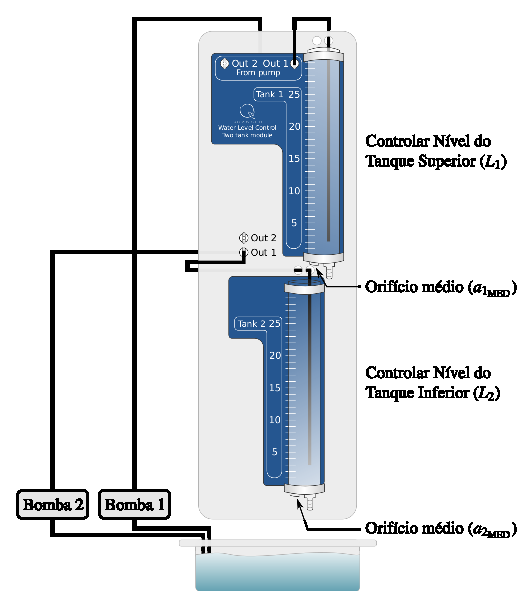
\includegraphics[width=0.45\textwidth]{imgs/sistema/eps/nova_config_1}
    \label{fig:nova_config_1}
}
\subfigure[Nova configuração 2.]
{
    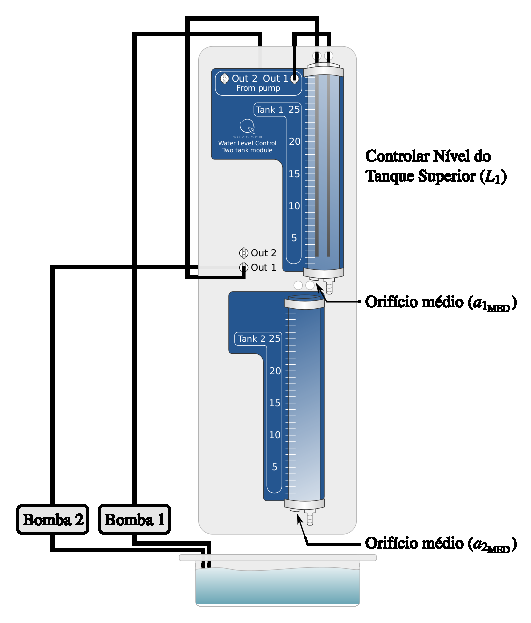
\includegraphics[width=0.45\textwidth]{imgs/sistema/eps/nova_config_2}
    \label{fig:nova_config_2}
}
\caption{Novas configurações sugeridas após a modificação do modelo.}
\label{fig:novas_config}
\end{figure}

Na configuração exposta pela Fig. \ref{fig:nova_config_1}, pode-se controlar o
nível dos dois tanques de maneira individual através das duas bombas de água.
Para isso, pode-se implementar dois controladores cada um com sua referência e a
leitura do respectivo sensor ou um único controlador que receberá as duas
referências e as leituras dos dois sensores.

Já na configuração exposta pela Fig. \ref{fig:nova_config_2}, a segunda bomba
está sendo utilizada para garantir que o processo continue funcionando
normalmente quando a primeira bomba vier a falhar. Ou seja, possui-se dois
atuadores com um deles em {\it standby}.  Ademais, ressalta-se que essa última
configuração pode ser adaptada para qualquer uma das três anteriores sugeridas
pelo fabricante.

Percebe-se que no primeiro caso (Fig. \ref{fig:nova_config_1}) o sistema deixa
de ser SISO e passa a ter múltiplas entradas e múltiplas saídas ({\it Multiple
Input and Multiple Output} -- MIMO). Por esse motivo, esse sistema será o
utilizado como modelo de estudo de caso no trabalho. A única modificação
existente nas equações que regem a dinâmica do modelo é a introdução de uma nova
variável na equação do segundo tanque em virtude da adição da segunda bomba.
Assim, as equações finais do modelo de estudo de caso serão:

\begin{eqnarray}
\dot{L_1} & = & \frac{K_m}{A}V_{p_{\tiny 1}} -
                \left[\frac{a_1}{A}\sqrt{2g}\right]\sqrt{L_1}
                \label{eq:l1_ponto}\\
\dot{L_2} & = & \frac{K_m}{A}V_{p_{\tiny 2}} +
                \left[\frac{a_1}{A}\sqrt{2g}\right]\sqrt{L_1} -
                \left[\frac{a_2}{A}\sqrt{2g}\right]\sqrt{L_2}
                \label{eq:l2_ponto}
\end{eqnarray}

\noindent em que $V_{p_{\tiny 1}}$ se refere à tensão aplicada na Bomba 1
($B_1$) e $V_{p_{\tiny 2}}$ à tensão aplicada na Bomba 2 ($B_2$).

\Glossary{$B_i$}{Bomba $i$}

% ------------------------------------------------------------------------------
\section{Limitações do processo}\label{sec:limitacoes}
Conforme dito anteriormente, a planta do estudo de caso foi desenvolvida para
fins acadêmicos e possui algumas limitações com relação as interfaces e aos
padrões de comunicação. Por causa dessas limitações a planta é normalmente
controlada por um sistema desenvolvido computacionalmente em que a comunicação
se dá através de um barramento ISA ({\it Industry Standard Architecture}). Tal
sistema deve calcular as ações de controle proporcional, integral e derivativa e
produzir um sinal de controle em Volts que será enviado aos atuadores.

\Glossary{ISA}{{\it Industry Standard Architecture}}

Entretanto, devido aos baixos níveis de tensão intrínsecos à esse tipo de
barramento, faz-se necessário utilizar um amplificador, também fornecido pela
Quanser\reg, com um fator de amplificação de cinco vezes. Assim, para que a
bomba não venha a queimar, os sistemas de controle devem implementar uma rotina
de segurança que garanta que o sinal de controle não supere os limites de $\pm
3$ Volts. A representação esquemática do funcionamento do sistema como um todo
está representada na Fig. \ref{fig:func_sistema}.

\begin{figure}[htb]
\centering
    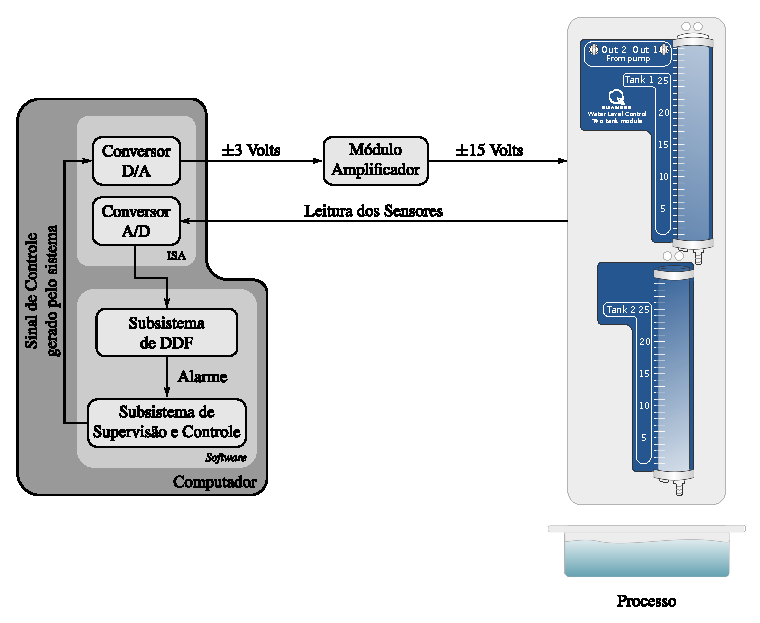
\includegraphics[width=0.8\textwidth]{imgs/sistema/eps/func_sistema}
    \caption{Diagrama esquemático de funcionamento do sistema proposto.}
    \label{fig:func_sistema}
\end{figure}

A partir dessa representação esquemática, percebe-se facilmente que as únicas
variáveis disponíveis são os níveis dos tanques ($L_1$ e $L_2$ e as tensões das
bombas ($V_{p_{\tiny 1}}$ e $V_{p_{\tiny 2}}$).

Além das limitações físicas relacionadas aos sinais enviados ou recebidos pelo
processo, destaca-se ainda o fato de se tratar de uma planta real em que todos
os dispositivos físicos e mecânicos estão sujeitos a deteriorações relacionadas
ao tempo de uso. Assim sendo, não se considera uma boa prática estimular ou
induzir falhas no sistema real. Logo, todas as falhas a serem analisadas serão
induzidas através do modelo matemático simulado em um sistema computacional.

% ------------------------------------------------------------------------------
\section{Simulações do sistema e das falhas}
Considerando os fatores expostos ao final da seção \ref{sec:limitacoes}, o
sistema de tanques será simulado a partir das Eqs. \ref{eq:l1_ponto} e
\ref{eq:l2_ponto}, utilizando o método de Runge-Kutta de 4\textordfeminine\
ordem (RK4).

\Glossary{RK4}{Método de Runge-Kutta de 4\textordfeminine\ ordem}

De maneira resumida, pode-se dizer que o RK4 faz parte de uma família de métodos
interativos para a aproximação numérica de soluções de equações diferenciais
ordinárias. O funcionamento do método pode esclarecido conforme explicação a
seguir. 

Seja um problema de valor inicial dado por:

\begin{equation}\label{eq:}
y' = f(t,y) \qquad y(t_0) = y_0
\end{equation}

Então o método RK4 para este problema é dado pelas seguintes equações:

\begin{eqnarray}
y_{n+1} & = & y_n + \frac{h}{6}\left(k_1 + 2k_2 + 2k_3 + k_4\right)\\
t_{n+1} & = & t_n + h
\end{eqnarray}

\noindent em que $y_{n+1}$ é a aproximação por RK4 de $y(t_{n + 1})$, e:

\begin{eqnarray}
k_1 & = & f\left(t_n,y_n\right)\\
k_2 & = & f\left(t_n+\frac{h}{2},y_n+\frac{h}{2}k_1\right)\\
k_3 & = & f\left(t_n+\frac{h}{2},y_n+\frac{h}{2}k_2\right)\\
k_4 & = & f\left(t_n+h,y_n+hk_3\right)
\end{eqnarray}

Assim, o próximo valor ($y_{n+1}$) é determinado a partir do valor atual ($y_n$)
somado com o produto do tamanho do intervalo ($h$) e uma inclinação estimada,
obtida a partir da média ponderada das inclinações $k_i$. Percebe-se ainda que a
média ponderada dá um maior peso para as inclinações no ponto médio.

\begin{comment}
\begin{itemize}
    \item $k_1$ é a inclinação no início do intervalo;
    \item $k_2$ é a inclinação no ponto médio do intervalo, usando $k_1$ para
determinar o valor de $y$ no ponto $t_n + h/2$ através do método de Euler;
    \item $k_3$ é novamente a inclinação no ponto médio do intervalo, usando
entretanto a inclinação $k_2$ para determinar o valor de $y$;
    \item $k_4$ é a inclinação no final do intervalo, com seu valor de $y$
determinado a partir de $k_3$.
\end{itemize}
\end{comment}

O método de RK4 permite que sejam determinados os valores de $L_1$ e $L_2$ para
cada instante da simulação e, consequentemente, que a dinâmica do processo seja
observada. As falhas induzidas no processo serão então computadas a partir de
alterações feitas sobre os valores de $L_1$ e $L_2$ obtidos. Dependendo do tipo
de falha, a alteração pode ocorrer antes, durante ou após a execução do método
de RK4.

% ------------------------------------------------------------------------------
\subsection{Falhas simuladas}
Assim como já foi visto, devido ao elevado grau de complexidade e à integração
inter processos, as falhas que antes poderiam ser detectadas através de medições
diretas de determinadas variáveis, passam a depender de um conjunto de variáveis
que atuam simultaneamente no sistema.  Ademais, as causas das falhas podem nem
sempre estar próximas dos locais em que foram identificadas.

Considerando tais aspectos, foram selecionadas somente algumas falhas dentre
aquelas que podem ocorrer no processo em estudo. Alguns exemplos de falhas desse
sistema podem ser observados na Tab. \ref{tab:selecao_falhas}. O agrupamento e a
classificação das falhas escolhidas se deu conforme Tabs.
\ref{tab:grupos_falhas} e \ref{tab:classificacao_falhas}.

\begin{table}[!htb]
\centering
\caption{Exemplos de falhas que podem ocorrer no sistema de tanques.}
\label{tab:selecao_falhas}
\vspace{0.25cm}
\begin{tabular}{|c|c|c|}
\hline
{\bf Sensores} & {\bf Atuadores} & {\bf Estruturais}\\
\hline
\hline
Erro de leitura & Erro de escrita & Erro de transmissão\\
\hline
Descalibramento & Erro de leitura & Perda de comunicação\\
\hline
Sensibilidade à ruído & Sensibilidade à ruído & Sensibilidade à ruído\\
\hline
Queima do sensor & Queima do atuador & Queima do transmissor\\
\hline
-- & Atraso de transporte & Atraso de propagação\\
\hline
\end{tabular}
\end{table}

\begin{table}[!htb]
\centering
\caption{Grupos de falhas.}
\label{tab:grupos_falhas}
\vspace{0.25cm}
\begin{tabular}{|c|c|c|}
\hline
{\bf Grupo} & {\bf Tipo de falha} & {\bf Sigla}\\
\hline
\hline
0 & Não há falhas & SF\\
\hline
1 & Falha do sensor & FSe\\
\hline
2 & Falha do atuador & FA\\
\hline
\multirow{2}{*}{3} & 
Falha estrutural ou & 
\multirow{2}{*}{FSi}\\
&
Falha do sistema & 
\\
\hline
\end{tabular}
\end{table}

\begin{table}[!htb]
\centering
\caption{Classificação das falhas selecionadas.}
\label{tab:classificacao_falhas}
\vspace{0.25cm}
\begin{tabular}{|c|c|c|c|c|}
\hline
{\bf Grupo} & {\bf Classe} & {\bf Denominação} & {\bf Variante} & {\bf Sigla}\\
\hline
\hline
1 & 1 & Descalibramento & Ganho & FSeDG\\
\hline
1 & 1 & Descalibramento & Nível DC ({\it offset}) & FSeDO\\
\hline
1 & 2 & Sensibilidade & Ruído & FSeSR\\
\hline
1 & 3 & Queima & -- & FSeQ\\
\hline
\hline
2 & 1 & Descalibramento & Ganho & FADG\\
\hline
2 & 1 & Descalibramento & Nível DC ({\it offset}) & FADO\\
\hline
2 & 2 & Sensibilidade & Ruído & FASR\\
\hline
2 & 3 & Variação & Constante da bomba ($K_m$) & FAVK\\
\hline
2 & 4 & Queima & -- & FAQ\\
\hline
\hline
3 & 3 & Vazamento & Tanque & FSiVzT\\
\hline
3 & 2 & Variação & Orifício de saída & FSiVrOS\\
\hline
3 & 2 & Variação & Ganho do módulo de potência & FSiVrGMP\\
\hline
3 & 1 & Entupimento & Orifício de saída & FSiEOS\\
\hline
\end{tabular}
\end{table}

\Glossary{FSeDG}{Falha do Sensor por Descalibramento de Ganho}
\Glossary{FSeDO}{Falha do Sensor por Descalibramento de {\it Offset}}
\Glossary{FSeSR}{Falha do Sensor por Sensibilidade à Ruído}
\Glossary{FSeQ}{Falha do Sensor por Queima}
\Glossary{FADG}{Falha do Atuador por Descalibramento de Ganho}
\Glossary{FADO}{Falha do Atuador por Descalibramento de {\it Offset}}
\Glossary{FASR}{Falha do Atuador por Sensibilidade à Ruído}
\Glossary{FAVK}{Falha do Atuador por Variação da Constante da Bomba ($K_m$)}
\Glossary{FAQ}{Falha do por Queima}
\Glossary{FSiVzT}{Falha do Sistema por Vazamento do Tanque}
\Glossary{FSiVrOS}{Falha do Sistema por Variação do Orifício de Saída}
\Glossary{FSiVrGMP}{Falha do Sistema por Variação do Ganho do Módulo de 
                    Potência}
\Glossary{FSiEOS}{Falha do Sistema por Entupimento do Orifício de Saída}

As siglas expostas nessas tabelas foram introduzidas com o intuito de facilitar
tanto o processo automático de treinamento e validação da estrutura neural,
quanto a referenciação textual.

As falhas expostas na Tab. \ref{tab:classificacao_falhas} são induzidas de
diferentes maneiras na simulação. Na FSeDG, por exemplo, o ganho do sensor é
alterado de 1,0 para qualquer outro valor a juízo do usuário no momento em que é
realizada a leitura dos níveis.

Para dar mais liberdade de configuração à simulação, foi desenvolvido um sistema
em C++, que implementa o método de RK4 e possui a capacidade de configurar todos
os parâmetros referentes a cada uma dessas falhas a partir de um arquivo de
texto. Cada um dos parâmetros do arquivo de entrada deve ser especificado em uma
coluna e o número de linhas equivale ao número de amostras a serem simuladas. O
período de amostragem utilizado na simulação do sistema é de 100
milissegundos, o mesmo que é utilizado na planta real.

Além disso, o sistema possui a implementação de dois controladores que podem ser
configurados para operarem como controladores P, PI, PD, PID ou PI-D. Os ganhos
proporcionais, integrais e derivativos são introduzidos na interface do usuário.

Esse mesmo sistema pode ainda ser utilizado para operar com a planta real,
fazendo aquisições dos dados através da rede (local ou remota), utilizando {\it
sockets} TCP, se comunicando com um servidor implementado conforme mostrado em
\citeasnoun{oliveira:2008}. A configuração do endereço IP e da porta de
comunicação também é realizada a partir da interface do usuário. A Fig.
\ref{fig:captura} mostra uma captura de tela ({\it screenshot}) do sistema em
funcionamento.

\begin{figure}[htb]
\centering
    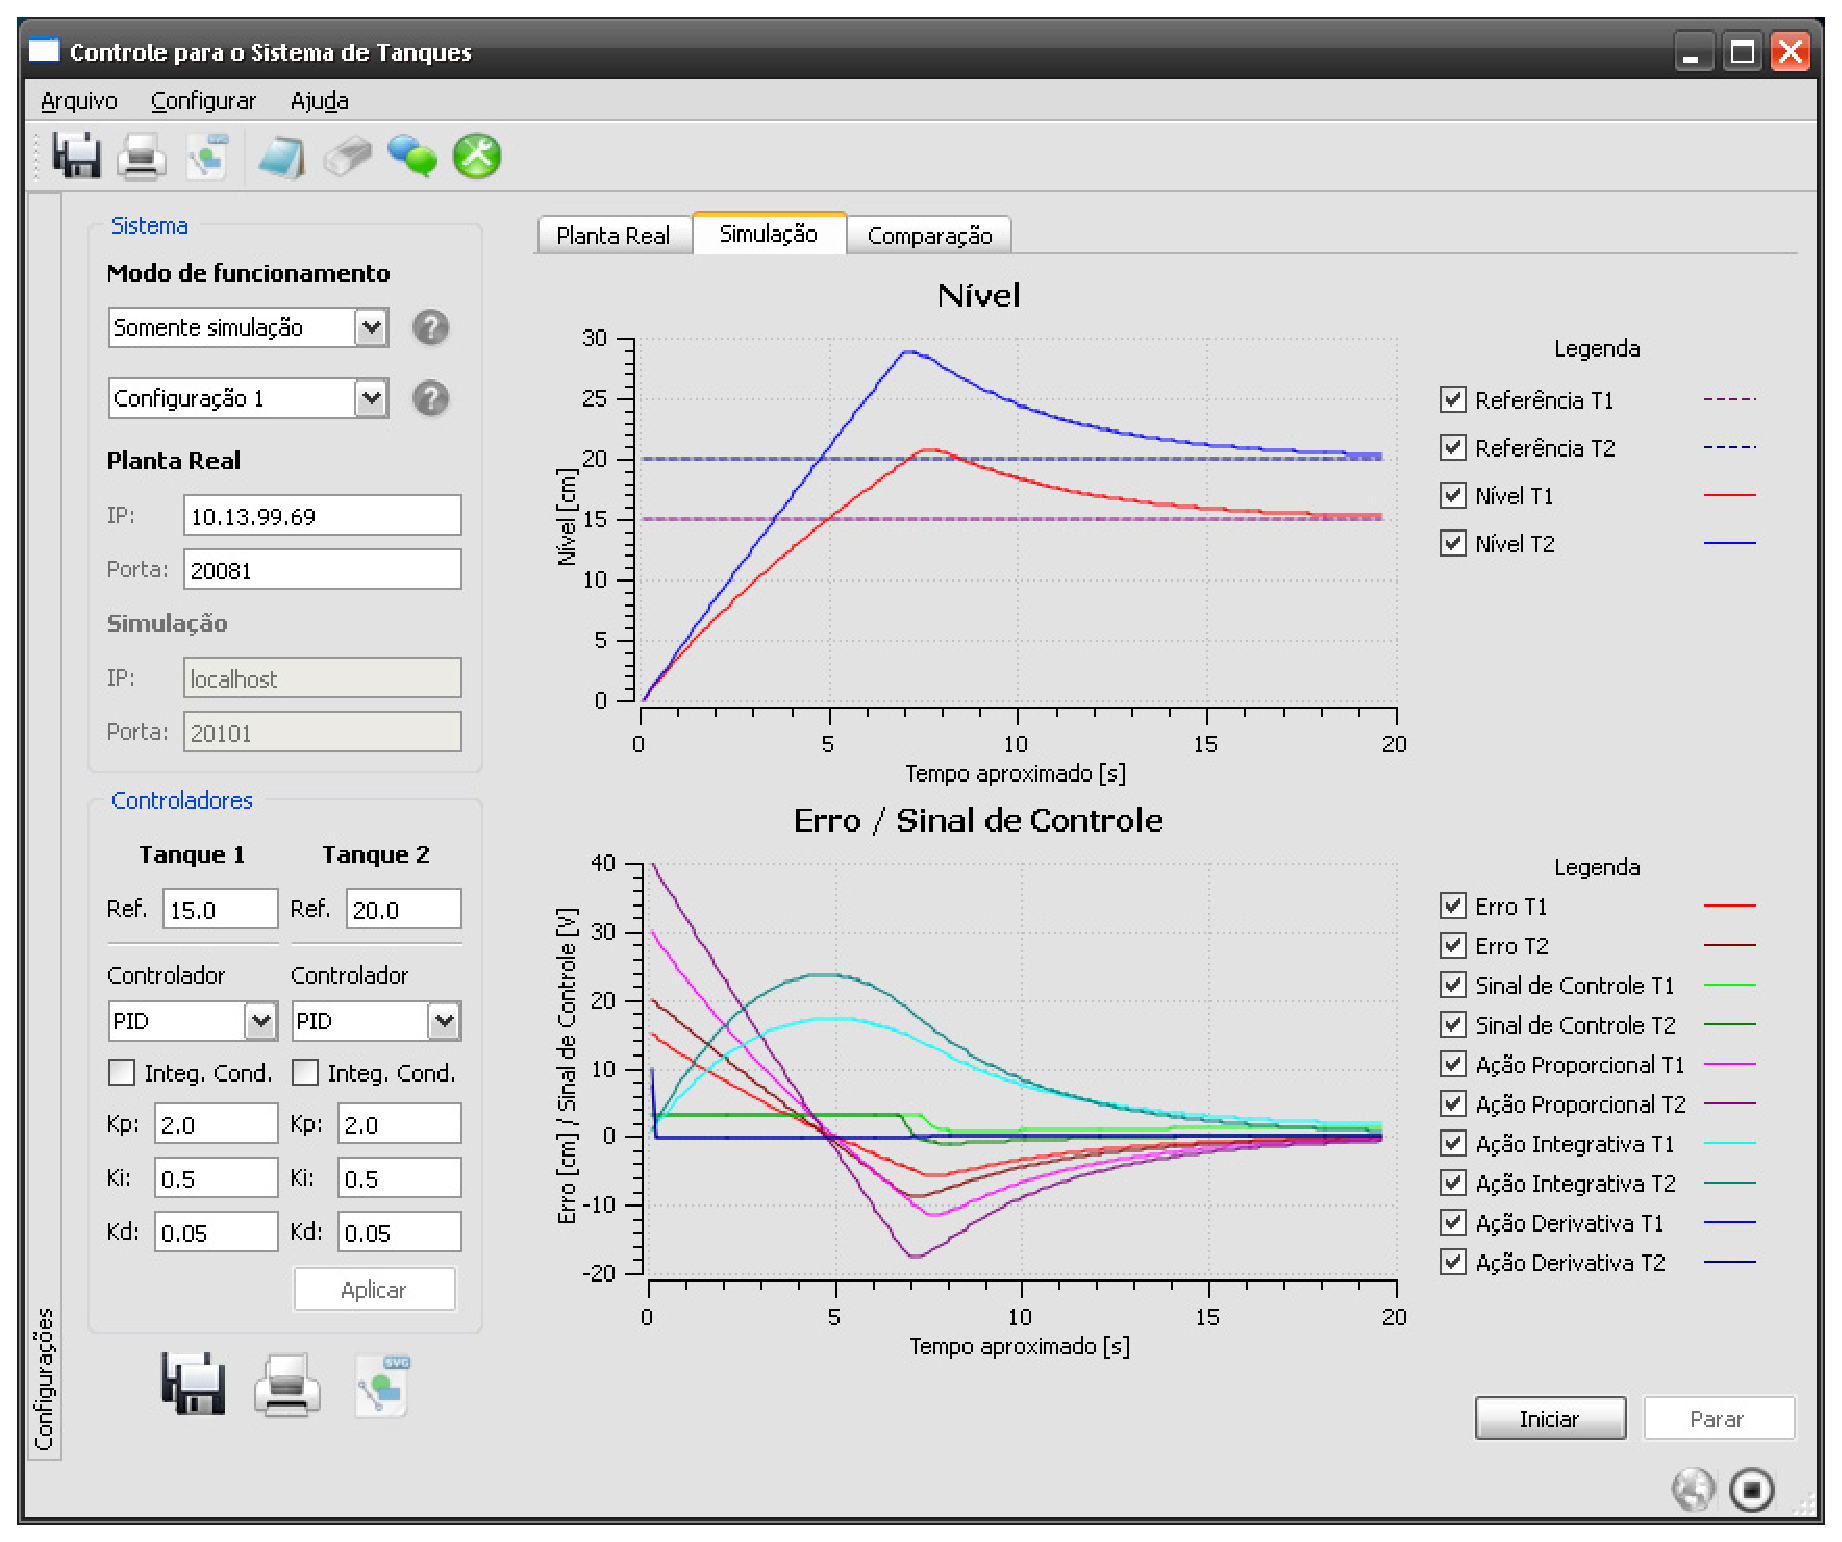
\includegraphics[width=0.75\textwidth]{imgs/sistema/eps/captura}
    \caption{Captura de tela do sistema de simulação em funcionamento.}
    \label{fig:captura}
\end{figure}

% ------------------------------------------------------------------------------
\section{Estruturas neurais escolhidas}
Tanto para a identificação do modelo quanto para a detecção e o diagnóstico das
falhas, deve-se ter bastante cuidado ao se escolher a estrutura e a arquitetura
das redes neurais. Em ambos os casos, uma escolha inadequada pode fazer com que
o sistema não se comporte de maneira adequada e não realize a função para o qual
foi designado. 

Assim sendo, para que fosse realizada uma análise comparativa, foram propostas
duas estruturas neurais para o processo de identificação do modelo e duas outras
estruturas para a detecção e o diagnóstico das falhas. Nos quatro casos foram
utilizados modelos NNARX com uma camada oculta com função de ativação sigmoidal
em que o número de regressores e o número de neurônios nessa camada foram
determinados a partir de testes, conforme mostrado no Cap. \ref{cap:resultados}.
Os detalhes relativos a cada uma dessas estruturas são esclarecidos nas próximas
seções.

% ------------------------------------------------------------------------------
\subsection{Propostas de identificação}
A primeira estrutura de identificação busca representar a dinâmica do sistema de
tanques através de uma única rede neural, a qual receberia como entrada os
valores passados dos níveis, $L_1(k-1)$ e $L_2(k-1)$, além dos valores de tensão
a serem aplicados, $V_{p_{\tiny 1}}(k)$ e $V_{p_{\tiny 2}}(k)$, gerando uma
estimativa dos níveis em sua saída. A Fig.  \ref{fig:ident_proposta_1}
representa um diagrama esquemático do funcionamento dessa primeira proposta.

\begin{figure}[htb]
\centering
    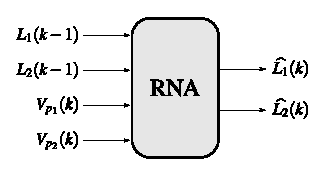
\includegraphics[width=0.4\textwidth]{imgs/sistema/eps/ident_proposta_1}
    \caption{Proposta de identificação global.}
    \label{fig:ident_proposta_1}
\end{figure}

Já a segunda estrutura de identificação leva em consideração que cada tanque
possui uma dinâmica diferente, tendo em vista que o $T_1$ age de maneira
independente, enquanto que a dinâmica de $T_2$ depende de $T_1$, conforme Eqs.
\ref{eq:l1_ponto} e \ref{eq:l2_ponto}. Assim, optou-se por utilizar duas redes
neurais, como mostrado na Fig. \ref{fig:ident_proposta_2}.

\begin{figure}[htb]
\centering
    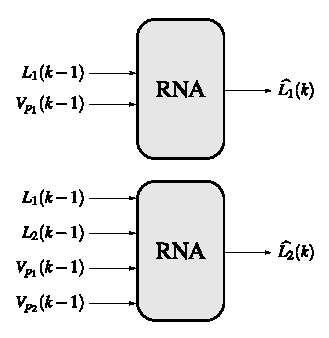
\includegraphics[width=0.4\textwidth]{imgs/sistema/eps/ident_proposta_2}
    \caption{Proposta de identificação individual.}
    \label{fig:ident_proposta_2}
\end{figure}

A primeira rede seria a responsável pela identificação de $T_1$, recebendo como
entrada o nível anterior, $L_1(k-1)$, e a tensão a ser aplicada, $V_{p_{\tiny
1}}(k)$, gerando uma estimativa de $L_1$ em sua saída. Já a segunda rede seria a
responsável pela identificação da dinâmica de $T_2$ e receberia como entrada as
mesmas variáveis da primeira proposta, ou seja, $L_1(k-1)$, $L_2(k-1)$,
$V_{p_{\tiny 1}}(k)$ e $V_{p_{\tiny 2}}(k)$. A saída da segunda rede seria,
portanto, a estimativa do nível de $T_2$.

Independentemente da proposta, pode-se visualizar o sistema de identificação do
modelo como uma única estrutura neural (simples ou composta), que possui como
entrada os níveis anteriores e as tensões a serem aplicadas, que produz em sua
saída as estimativas dos níveis dos dois tanques. A Fig. \ref{fig:sist_ident}
mostra como o sistema de identificação pode ser visto.

\begin{figure}[!htb]
\centering
    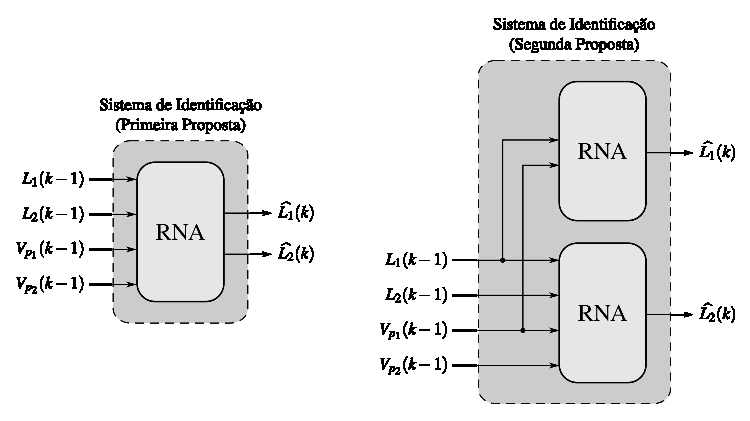
\includegraphics[width=0.9\textwidth]{imgs/sistema/eps/sist_ident}
    \caption{Visão geral do sistema de identificação.}
    \label{fig:sist_ident}
\end{figure}

% ------------------------------------------------------------------------------
\subsection{Propostas de detecção}
As estruturas neurais de DDF seguiram o mesmo raciocínio adotado para as
estruturas de identificação. No primeiro caso, buscou-se desenvolver uma
única rede neural que fosse capaz de detectar e identificar cada das falhas
listas pela Tab. \ref{tab:classificacao_falhas}. Essa rede receberia como
entrada os mesmos sinais das redes de identificação além dos resíduos produzidos
pela diferença dos níveis entre o modelo simulado ($L_i$) e o modelo
identificado ($\widehat{L_i}$). A saída da rede formaria uma palavra binária que
seria decodificada a partir de uma tabela previamente estabelecida. Nessa tabela
cada falha teria uma palavra binária correspondente. A Fig.
\ref{fig:detec_prop_1} representa um diagrama esquemático dessa proposta.

\begin{figure}[!htb]
\centering
    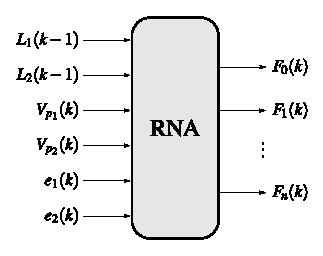
\includegraphics[width=0.38\textwidth]{imgs/sistema/eps/detec_prop_1}
    \caption{Proposta de detecção através de uma única rede neural.}
    \label{fig:detec_prop_1}
\end{figure}

Na segunda proposta, a estrutura de DDF seria composta por várias redes neurais,
em que cada uma destas estaria associada a uma única falha, formando um conjunto
de ``especialistas''. Não se trata entretanto de uma máquina de comitê de
especialistas por não existir uma outra rede que realizaria a tomada de
decisões. Inicialmente, as entradas de cada uma das redes seriam as mesmas da
primeira proposta. As saídas, por sua vez, seriam compostas por uma palavra de
apenas 2 bits, indicando se aquela falha estaria sendo detectada cada em $T_1$
em $T_2$ ou em $T_1$ e $T_2$ simultaneamente. A Fig. \ref{fig:detec_prop_2}
representa um diagrama esquemático dessa proposta.

\begin{figure}[!htb]
\centering
    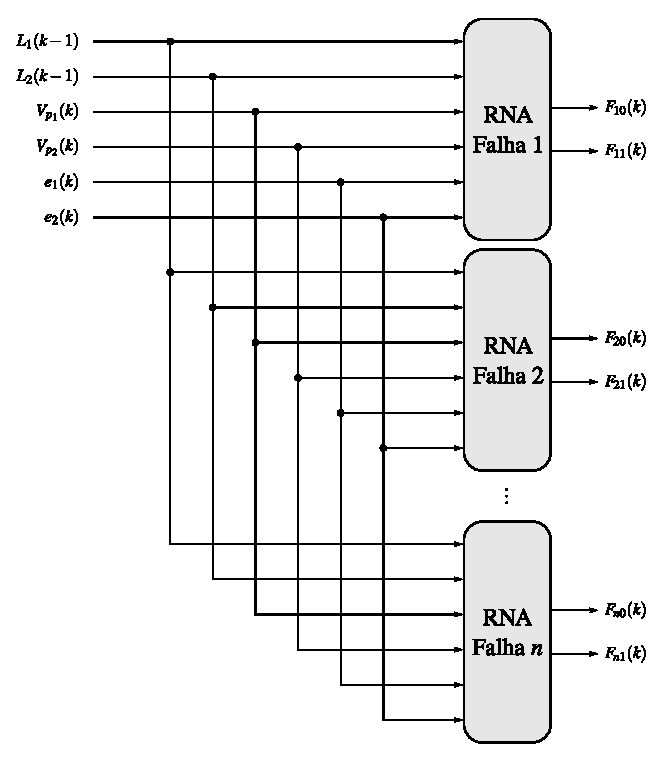
\includegraphics[width=0.725\textwidth]{imgs/sistema/eps/detec_prop_2}
    \caption{Proposta de detecção através de um conjunto de redes
             especialistas.}
    \label{fig:detec_prop_2}
\end{figure}

Existem diversas vantagens em se utilizar a segunda proposta ao invés da
primeira, como por exemplo, a de se utilizar entradas diferentes para cada uma
das redes especialistas. Essa situação poderia ocorrer se fosse percebido que
uma determinada entrada, ao ser adicionada, fizesse com que aquela falha fosse
detectada de maneira mais precisa e rápida. Ou então na situação inversa, em que
uma determinada entrada não estivesse fazendo diferença com relação ao processo
de detecção.

Modificar a estrutura das entradas na primeira proposta faria com que a rede
precisasse ser treinada novamente. Por se tratar, provavelmente, de uma
estrutura mais complexa, o treinamento poderia ter um grande custo relacionado
ao tempo e ao processamento. Já na segunda proposta apenas uma das redes seria
retreinada, o que iria reduzir esse custo de maneira considerável. Além disso,
se o treinamento fosse realizado em tempo real, não haveria necessidade de se
parar o sistema de detecção como um todo, mas somente uma parte deste. 

Uma outra vantagem estaria relacionada com o pós-processamento da informação. Ao
se utilizar a segunda proposta percebe-se que não será realizar uma
decodificação da saída cada vez que uma entrada for introduzida na rede.
Considerando que o tempo gasto para se decodificar a palavra gerada na saída da
primeira proposta, é diretamente proporcional ao tamanho da palavra que, por sua
vez, está diretamente relacionado ao número de falhas a serem identificadas,
pode-se dizer que quanto maior for o número de falhas a serem identificadas
maior será esse tempo de decodificação.

Além desse fator, vale ainda salientar que as falhas podem acontecer de maneira
simultânea e independente, o que iria produzir um grande número de combinações
de falhas. Para um conjunto de 13 (treze) falhas, por exemplo, considerando que
somente 2 (duas) destas poderiam atuar simultaneamente, teria-se um total de 78
(setenta e oito) combinações distintas. Se todas as combinações fossem
consideradas esse número cresceria de maneira exorbitante.

Como cada uma dessas combinações deve ser identificada de maneira única pelo
sistema, há então a necessidade de se representar as combinações dentre as
palavras de saída. Assim, além das palavras binárias que representariam cada uma
das falhas, precisariam existir as palavras binárias que representariam as
combinações de cada uma dessas, aumentando ainda mais o número de bits e,
consequentemente o tempo de decodificação.

Um outro ponto que pode ser destacado é que ao se utilizar a segunda proposta,
torna-se mais fácil realizar o acoplamento do sistema de DDF com um sistema de
monitoramento e geração de alarme, pois cada falha seria acionada de maneira
individual. Assim, os sinais de acionamento poderiam conter informações
pertinentes para que os respectivos alarmes fossem gerados de maneira mais
precisa.

Apesar dessas vantagens, será feita uma análise comparativa dos resultados
dessas estruturas. Dessa forma pode-se determinar qual das duas propostas melhor
se adaptaria para o estudo de caso.

Assim como o sistema de identificação, o sistema de detecção também pode ser
visto como uma única estrutura neural. A única observação a ser feita é que a
saída dessa estrutura poderá ser uma palavra binária de $p$ bits, tal que $2^p
\geq n$, em que $n$ representa o número de palavras a serem identificadas; ou
$n$ palavras binárias de 2 bits. Nesse último caso $n$ representa simplesmente o
número de falhas a serem identificadas, pois as combinações de falhas são
obtidas a partir das saídas ativas de cada uma das redes.

% ------------------------------------------------------------------------------
\section{Composição do sistema}
Tendo conhecido todos os subsistemas a serem utilizados, pode-se observar na
Fig. \ref{fig:composicao} a estrutura do sistema de DDF proposto. Deve-se
destacar entretanto que o trabalho aqui proposto não incorpora o desenvolvimento
de um sistema de supervisão e monitoramento completo, mas somente o sistema de
DDF.

\begin{figure}[htb]
\centering
    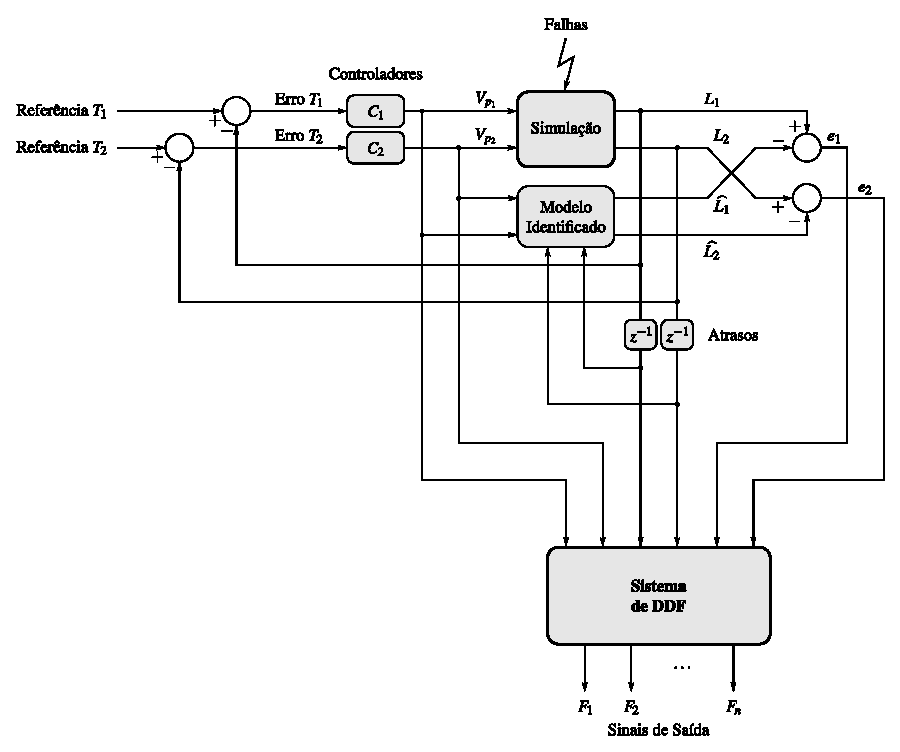
\includegraphics[width=0.9\textwidth]{imgs/sistema/eps/composicao}
    \caption{Composição do sistema proposto.}
    \label{fig:composicao}
\end{figure}

Acoplar tal sistema à um ambiente de monitoramento e supervisão, ou ainda
associá-lo à técnicas de controle tolerante à falhas, consiste simplesmente em
processar as informações disponíveis na interface de saída do módulo de DDF.

\mychapter{Resultados parciais}
\label{cap:resultados}

% Dados para as simulações da qualificação
% Tempo de simulação de 105 segundos (totalizando 00:01:45)
% Valores utilizados => Observar folha


% Montar tabela com os valores dos parametros alterados para o treinamento e
% para a validação das falhas. Exemplo:
% 
% FAVK => km_treinamento = (0.7 a 1.1)*km_original (PRBS)
%         km_validacao = (0.75 a 1.05)*km_original (PRBS) => nao precisa
%                                                            especificar o valor
%                                                            exato, mas dizer
%                                                            que estava dentro
%                                                            da faixa do
%                                                            treinamento
%         km_resultado = (0.75)*km_original (Fixo)
%
% FSeDG => ganho_treinamento = (1 +- 0.2)*ganho_original (PRBS)
%          ganho_validacao = (1 +- 0.15)*ganho_original (PRBS)
%          ganho_resultado = 0.8*ganho_original (fixo)
%


% Mostrar que foram feitos 3 conjuntos de validacao e depois foram escolhidas as
% melhores redes => Mostrar tabelas com Falso positivo e falso negativo


% Quando for falar sobre o número de regressores escolhidos => Dizer que
% considere que os regressores estão representados internamente ao "sistema de
% identificação" e ao "sistema de DDF" na figura da composição do sistema (final
% do cap:sistema)

\begin{comment}
Neste capítulo será realizada uma análise comparativa dos resultados obtidos nas
duas propostas do sistema de DDF. Ao final, do capítulo a melhor estrutura será
escolhida para que seja feita uma análise mais detalhada dos resultados.
\end{comment}

Neste capítulo serão analisados os resultados parciais obtidos a partir da
implementação da segunda proposta do sistema de DDF. Para isso, em um primeiro
momento será mostrado como se deu a coleta dos dados de treinamento e validação
das redes especialistas e em seguida será feita uma comparação de desempenho. Ao
final do capítulo as melhores estruturas serão selecionadas para que se realize
uma análise um pouco mais detalhada acerca da detecção das falhas.

% ------------------------------------------------------------------------------
\section{Coleta dos dados}

% ------------------------------------------------------------------------------
\subsection{Simulações computacionais}

% ------------------------------------------------------------------------------
%\subsection{Método de Runge-Kutta de 4\textordfeminine ordem}

% ------------------------------------------------------------------------------
\section{Análise das RNAs}

% ------------------------------------------------------------------------------
\subsection{Identificação}

% ------------------------------------------------------------------------------
\subsection{Detecção de falhas}

% ------------------------------------------------------------------------------
\section{Melhores redes}

% ------------------------------------------------------------------------------
\section{Composição final}

% ------------------------------------------------------------------------------
\section{Detecções}

% ------------------------------------------------------------------------------
\section{Comparação das propostas}

% Falhas nos sensores ..........................................................
\begin{figure}[htb]
\footnotesize
\centering
% GNUPLOT: LaTeX picture with Postscript
\begingroup
  \makeatletter
  \providecommand\color[2][]{%
    \GenericError{(gnuplot) \space\space\space\@spaces}{%
      Package color not loaded in conjunction with
      terminal option `colourtext'%
    }{See the gnuplot documentation for explanation.%
    }{Either use 'blacktext' in gnuplot or load the package
      color.sty in LaTeX.}%
    \renewcommand\color[2][]{}%
  }%
  \providecommand\includegraphics[2][]{%
    \GenericError{(gnuplot) \space\space\space\@spaces}{%
      Package graphicx or graphics not loaded%
    }{See the gnuplot documentation for explanation.%
    }{The gnuplot epslatex terminal needs graphicx.sty or graphics.sty.}%
    \renewcommand\includegraphics[2][]{}%
  }%
  \providecommand\rotatebox[2]{#2}%
  \@ifundefined{ifGPcolor}{%
    \newif\ifGPcolor
    \GPcolortrue
  }{}%
  \@ifundefined{ifGPblacktext}{%
    \newif\ifGPblacktext
    \GPblacktexttrue
  }{}%
  % define a \g@addto@macro without @ in the name:
  \let\gplgaddtomacro\g@addto@macro
  % define empty templates for all commands taking text:
  \gdef\gplbacktext{}%
  \gdef\gplfronttext{}%
  \makeatother
  \ifGPblacktext
    % no textcolor at all
    \def\colorrgb#1{}%
    \def\colorgray#1{}%
  \else
    % gray or color?
    \ifGPcolor
      \def\colorrgb#1{\color[rgb]{#1}}%
      \def\colorgray#1{\color[gray]{#1}}%
      \expandafter\def\csname LTw\endcsname{\color{white}}%
      \expandafter\def\csname LTb\endcsname{\color{black}}%
      \expandafter\def\csname LTa\endcsname{\color{black}}%
      \expandafter\def\csname LT0\endcsname{\color[rgb]{1,0,0}}%
      \expandafter\def\csname LT1\endcsname{\color[rgb]{0,1,0}}%
      \expandafter\def\csname LT2\endcsname{\color[rgb]{0,0,1}}%
      \expandafter\def\csname LT3\endcsname{\color[rgb]{1,0,1}}%
      \expandafter\def\csname LT4\endcsname{\color[rgb]{0,1,1}}%
      \expandafter\def\csname LT5\endcsname{\color[rgb]{1,1,0}}%
      \expandafter\def\csname LT6\endcsname{\color[rgb]{0,0,0}}%
      \expandafter\def\csname LT7\endcsname{\color[rgb]{1,0.3,0}}%
      \expandafter\def\csname LT8\endcsname{\color[rgb]{0.5,0.5,0.5}}%
    \else
      % gray
      \def\colorrgb#1{\color{black}}%
      \def\colorgray#1{\color[gray]{#1}}%
      \expandafter\def\csname LTw\endcsname{\color{white}}%
      \expandafter\def\csname LTb\endcsname{\color{black}}%
      \expandafter\def\csname LTa\endcsname{\color{black}}%
      \expandafter\def\csname LT0\endcsname{\color{black}}%
      \expandafter\def\csname LT1\endcsname{\color{black}}%
      \expandafter\def\csname LT2\endcsname{\color{black}}%
      \expandafter\def\csname LT3\endcsname{\color{black}}%
      \expandafter\def\csname LT4\endcsname{\color{black}}%
      \expandafter\def\csname LT5\endcsname{\color{black}}%
      \expandafter\def\csname LT6\endcsname{\color{black}}%
      \expandafter\def\csname LT7\endcsname{\color{black}}%
      \expandafter\def\csname LT8\endcsname{\color{black}}%
    \fi
  \fi
  \setlength{\unitlength}{0.0500bp}%
  \begin{picture}(7200.00,5040.00)%
    \gplgaddtomacro\gplbacktext{%
      \csname LTb\endcsname%
      \put(726,3150){\makebox(0,0)[r]{\strut{} 5}}%
      \csname LTb\endcsname%
      \put(726,3780){\makebox(0,0)[r]{\strut{} 10}}%
      \csname LTb\endcsname%
      \put(726,4409){\makebox(0,0)[r]{\strut{} 15}}%
      \csname LTb\endcsname%
      \put(726,5039){\makebox(0,0)[r]{\strut{} 20}}%
      \csname LTb\endcsname%
      \put(921,2237){\makebox(0,0){\strut{}}}%
      \csname LTb\endcsname%
      \put(1771,2237){\makebox(0,0){\strut{}}}%
      \csname LTb\endcsname%
      \put(2620,2237){\makebox(0,0){\strut{}}}%
      \csname LTb\endcsname%
      \put(3470,2237){\makebox(0,0){\strut{}}}%
      \csname LTb\endcsname%
      \put(4320,2237){\makebox(0,0){\strut{}}}%
      \csname LTb\endcsname%
      \put(5170,2237){\makebox(0,0){\strut{}}}%
      \csname LTb\endcsname%
      \put(6019,2237){\makebox(0,0){\strut{}}}%
      \csname LTb\endcsname%
      \put(6869,2237){\makebox(0,0){\strut{}}}%
      \put(352,3779){\rotatebox{-270}{\makebox(0,0){\strut{}Nível [cm]}}}%
    }%
    \gplgaddtomacro\gplfronttext{%
      \csname LTb\endcsname%
      \put(6278,2913){\makebox(0,0)[r]{\strut{}Ref. $T_1$}}%
      \csname LTb\endcsname%
      \put(6278,2693){\makebox(0,0)[r]{\strut{}Saída $T_1$}}%
    }%
    \gplgaddtomacro\gplbacktext{%
      \csname LTb\endcsname%
      \put(726,0){\makebox(0,0)[r]{\strut{} 0}}%
      \csname LTb\endcsname%
      \put(726,420){\makebox(0,0)[r]{\strut{} 5}}%
      \csname LTb\endcsname%
      \put(726,840){\makebox(0,0)[r]{\strut{} 10}}%
      \csname LTb\endcsname%
      \put(726,1260){\makebox(0,0)[r]{\strut{} 15}}%
      \csname LTb\endcsname%
      \put(726,1680){\makebox(0,0)[r]{\strut{} 20}}%
      \csname LTb\endcsname%
      \put(726,2100){\makebox(0,0)[r]{\strut{} 25}}%
      \csname LTb\endcsname%
      \put(726,2520){\makebox(0,0)[r]{\strut{} 30}}%
      \csname LTb\endcsname%
      \put(921,-283){\makebox(0,0){\strut{}0}}%
      \csname LTb\endcsname%
      \put(1771,-283){\makebox(0,0){\strut{}15}}%
      \csname LTb\endcsname%
      \put(2620,-283){\makebox(0,0){\strut{}30}}%
      \csname LTb\endcsname%
      \put(3470,-283){\makebox(0,0){\strut{}45}}%
      \csname LTb\endcsname%
      \put(4320,-283){\makebox(0,0){\strut{}60}}%
      \csname LTb\endcsname%
      \put(5170,-283){\makebox(0,0){\strut{}75}}%
      \csname LTb\endcsname%
      \put(6019,-283){\makebox(0,0){\strut{}90}}%
      \csname LTb\endcsname%
      \put(6869,-283){\makebox(0,0){\strut{}105}}%
      \put(352,1260){\rotatebox{-270}{\makebox(0,0){\strut{}Nível [cm]}}}%
      \put(3895,-613){\makebox(0,0){\strut{}Tempo [s]}}%
    }%
    \gplgaddtomacro\gplfronttext{%
      \csname LTb\endcsname%
      \put(6278,393){\makebox(0,0)[r]{\strut{}Ref. $T_2$}}%
      \csname LTb\endcsname%
      \put(6278,173){\makebox(0,0)[r]{\strut{}Saída $T_2$}}%
    }%
    \gplbacktext
    \put(0,0){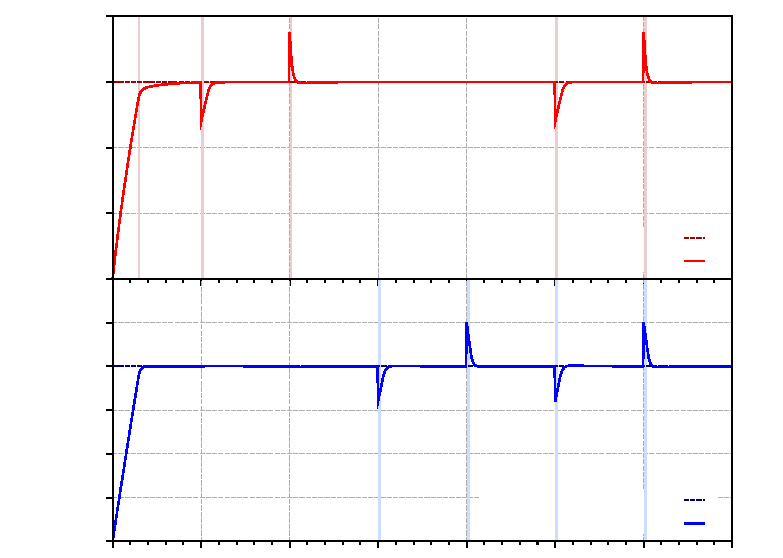
\includegraphics{fsedg}}%
    \gplfronttext
  \end{picture}%
\endgroup

\vspace{1cm}
\caption{FSeDG (80\%)}
\label{fig:fsedg}
\end{figure}

\begin{figure}[htb]
\footnotesize
\centering
% GNUPLOT: LaTeX picture with Postscript
\begingroup
  \makeatletter
  \providecommand\color[2][]{%
    \GenericError{(gnuplot) \space\space\space\@spaces}{%
      Package color not loaded in conjunction with
      terminal option `colourtext'%
    }{See the gnuplot documentation for explanation.%
    }{Either use 'blacktext' in gnuplot or load the package
      color.sty in LaTeX.}%
    \renewcommand\color[2][]{}%
  }%
  \providecommand\includegraphics[2][]{%
    \GenericError{(gnuplot) \space\space\space\@spaces}{%
      Package graphicx or graphics not loaded%
    }{See the gnuplot documentation for explanation.%
    }{The gnuplot epslatex terminal needs graphicx.sty or graphics.sty.}%
    \renewcommand\includegraphics[2][]{}%
  }%
  \providecommand\rotatebox[2]{#2}%
  \@ifundefined{ifGPcolor}{%
    \newif\ifGPcolor
    \GPcolortrue
  }{}%
  \@ifundefined{ifGPblacktext}{%
    \newif\ifGPblacktext
    \GPblacktexttrue
  }{}%
  % define a \g@addto@macro without @ in the name:
  \let\gplgaddtomacro\g@addto@macro
  % define empty templates for all commands taking text:
  \gdef\gplbacktext{}%
  \gdef\gplfronttext{}%
  \makeatother
  \ifGPblacktext
    % no textcolor at all
    \def\colorrgb#1{}%
    \def\colorgray#1{}%
  \else
    % gray or color?
    \ifGPcolor
      \def\colorrgb#1{\color[rgb]{#1}}%
      \def\colorgray#1{\color[gray]{#1}}%
      \expandafter\def\csname LTw\endcsname{\color{white}}%
      \expandafter\def\csname LTb\endcsname{\color{black}}%
      \expandafter\def\csname LTa\endcsname{\color{black}}%
      \expandafter\def\csname LT0\endcsname{\color[rgb]{1,0,0}}%
      \expandafter\def\csname LT1\endcsname{\color[rgb]{0,1,0}}%
      \expandafter\def\csname LT2\endcsname{\color[rgb]{0,0,1}}%
      \expandafter\def\csname LT3\endcsname{\color[rgb]{1,0,1}}%
      \expandafter\def\csname LT4\endcsname{\color[rgb]{0,1,1}}%
      \expandafter\def\csname LT5\endcsname{\color[rgb]{1,1,0}}%
      \expandafter\def\csname LT6\endcsname{\color[rgb]{0,0,0}}%
      \expandafter\def\csname LT7\endcsname{\color[rgb]{1,0.3,0}}%
      \expandafter\def\csname LT8\endcsname{\color[rgb]{0.5,0.5,0.5}}%
    \else
      % gray
      \def\colorrgb#1{\color{black}}%
      \def\colorgray#1{\color[gray]{#1}}%
      \expandafter\def\csname LTw\endcsname{\color{white}}%
      \expandafter\def\csname LTb\endcsname{\color{black}}%
      \expandafter\def\csname LTa\endcsname{\color{black}}%
      \expandafter\def\csname LT0\endcsname{\color{black}}%
      \expandafter\def\csname LT1\endcsname{\color{black}}%
      \expandafter\def\csname LT2\endcsname{\color{black}}%
      \expandafter\def\csname LT3\endcsname{\color{black}}%
      \expandafter\def\csname LT4\endcsname{\color{black}}%
      \expandafter\def\csname LT5\endcsname{\color{black}}%
      \expandafter\def\csname LT6\endcsname{\color{black}}%
      \expandafter\def\csname LT7\endcsname{\color{black}}%
      \expandafter\def\csname LT8\endcsname{\color{black}}%
    \fi
  \fi
  \setlength{\unitlength}{0.0500bp}%
  \begin{picture}(7200.00,5040.00)%
    \gplgaddtomacro\gplbacktext{%
      \csname LTb\endcsname%
      \put(726,3150){\makebox(0,0)[r]{\strut{} 5}}%
      \csname LTb\endcsname%
      \put(726,3780){\makebox(0,0)[r]{\strut{} 10}}%
      \csname LTb\endcsname%
      \put(726,4409){\makebox(0,0)[r]{\strut{} 15}}%
      \csname LTb\endcsname%
      \put(726,5039){\makebox(0,0)[r]{\strut{} 20}}%
      \csname LTb\endcsname%
      \put(921,2237){\makebox(0,0){\strut{}}}%
      \csname LTb\endcsname%
      \put(1771,2237){\makebox(0,0){\strut{}}}%
      \csname LTb\endcsname%
      \put(2620,2237){\makebox(0,0){\strut{}}}%
      \csname LTb\endcsname%
      \put(3470,2237){\makebox(0,0){\strut{}}}%
      \csname LTb\endcsname%
      \put(4320,2237){\makebox(0,0){\strut{}}}%
      \csname LTb\endcsname%
      \put(5170,2237){\makebox(0,0){\strut{}}}%
      \csname LTb\endcsname%
      \put(6019,2237){\makebox(0,0){\strut{}}}%
      \csname LTb\endcsname%
      \put(6869,2237){\makebox(0,0){\strut{}}}%
      \put(352,3779){\rotatebox{-270}{\makebox(0,0){\strut{}Level [cm]}}}%
    }%
    \gplgaddtomacro\gplfronttext{%
      \csname LTb\endcsname%
      \put(6278,2913){\makebox(0,0)[r]{\strut{}Setpoint $T_1$}}%
      \csname LTb\endcsname%
      \put(6278,2693){\makebox(0,0)[r]{\strut{}Output $T_1$}}%
    }%
    \gplgaddtomacro\gplbacktext{%
      \csname LTb\endcsname%
      \put(726,0){\makebox(0,0)[r]{\strut{} 0}}%
      \csname LTb\endcsname%
      \put(726,504){\makebox(0,0)[r]{\strut{} 5}}%
      \csname LTb\endcsname%
      \put(726,1008){\makebox(0,0)[r]{\strut{} 10}}%
      \csname LTb\endcsname%
      \put(726,1512){\makebox(0,0)[r]{\strut{} 15}}%
      \csname LTb\endcsname%
      \put(726,2016){\makebox(0,0)[r]{\strut{} 20}}%
      \csname LTb\endcsname%
      \put(726,2520){\makebox(0,0)[r]{\strut{} 25}}%
      \csname LTb\endcsname%
      \put(921,-283){\makebox(0,0){\strut{}0}}%
      \csname LTb\endcsname%
      \put(1771,-283){\makebox(0,0){\strut{}15}}%
      \csname LTb\endcsname%
      \put(2620,-283){\makebox(0,0){\strut{}30}}%
      \csname LTb\endcsname%
      \put(3470,-283){\makebox(0,0){\strut{}45}}%
      \csname LTb\endcsname%
      \put(4320,-283){\makebox(0,0){\strut{}60}}%
      \csname LTb\endcsname%
      \put(5170,-283){\makebox(0,0){\strut{}75}}%
      \csname LTb\endcsname%
      \put(6019,-283){\makebox(0,0){\strut{}90}}%
      \csname LTb\endcsname%
      \put(6869,-283){\makebox(0,0){\strut{}105}}%
      \put(352,1260){\rotatebox{-270}{\makebox(0,0){\strut{}Level [cm]}}}%
      \put(3895,-613){\makebox(0,0){\strut{}Time [s]}}%
    }%
    \gplgaddtomacro\gplfronttext{%
      \csname LTb\endcsname%
      \put(6278,393){\makebox(0,0)[r]{\strut{}Setpoint $T_2$}}%
      \csname LTb\endcsname%
      \put(6278,173){\makebox(0,0)[r]{\strut{}Output $T_2$}}%
    }%
    \gplbacktext
    \put(0,0){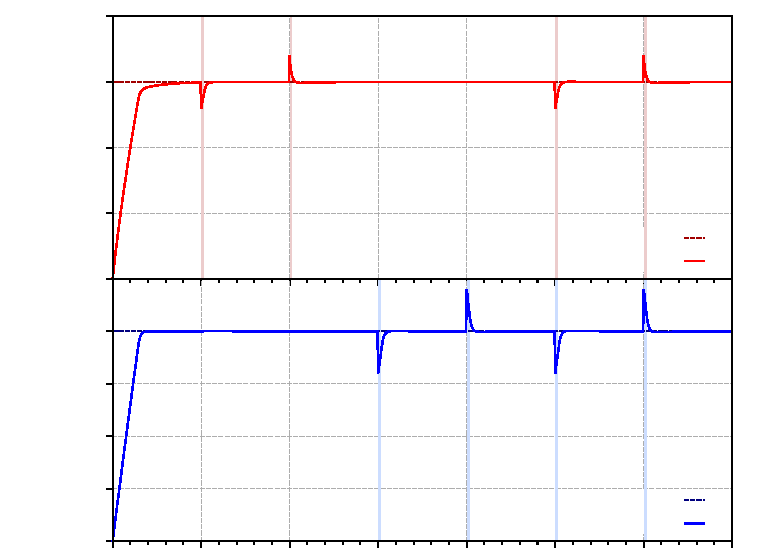
\includegraphics{fsedo}}%
    \gplfronttext
  \end{picture}%
\endgroup

\vspace{1cm}
\caption{FSeDO (-2 cm)}
\label{fig:fsedo}
\end{figure}

\begin{figure}[htb]
\footnotesize
\centering
% GNUPLOT: LaTeX picture with Postscript
\begingroup
  \makeatletter
  \providecommand\color[2][]{%
    \GenericError{(gnuplot) \space\space\space\@spaces}{%
      Package color not loaded in conjunction with
      terminal option `colourtext'%
    }{See the gnuplot documentation for explanation.%
    }{Either use 'blacktext' in gnuplot or load the package
      color.sty in LaTeX.}%
    \renewcommand\color[2][]{}%
  }%
  \providecommand\includegraphics[2][]{%
    \GenericError{(gnuplot) \space\space\space\@spaces}{%
      Package graphicx or graphics not loaded%
    }{See the gnuplot documentation for explanation.%
    }{The gnuplot epslatex terminal needs graphicx.sty or graphics.sty.}%
    \renewcommand\includegraphics[2][]{}%
  }%
  \providecommand\rotatebox[2]{#2}%
  \@ifundefined{ifGPcolor}{%
    \newif\ifGPcolor
    \GPcolortrue
  }{}%
  \@ifundefined{ifGPblacktext}{%
    \newif\ifGPblacktext
    \GPblacktexttrue
  }{}%
  % define a \g@addto@macro without @ in the name:
  \let\gplgaddtomacro\g@addto@macro
  % define empty templates for all commands taking text:
  \gdef\gplbacktext{}%
  \gdef\gplfronttext{}%
  \makeatother
  \ifGPblacktext
    % no textcolor at all
    \def\colorrgb#1{}%
    \def\colorgray#1{}%
  \else
    % gray or color?
    \ifGPcolor
      \def\colorrgb#1{\color[rgb]{#1}}%
      \def\colorgray#1{\color[gray]{#1}}%
      \expandafter\def\csname LTw\endcsname{\color{white}}%
      \expandafter\def\csname LTb\endcsname{\color{black}}%
      \expandafter\def\csname LTa\endcsname{\color{black}}%
      \expandafter\def\csname LT0\endcsname{\color[rgb]{1,0,0}}%
      \expandafter\def\csname LT1\endcsname{\color[rgb]{0,1,0}}%
      \expandafter\def\csname LT2\endcsname{\color[rgb]{0,0,1}}%
      \expandafter\def\csname LT3\endcsname{\color[rgb]{1,0,1}}%
      \expandafter\def\csname LT4\endcsname{\color[rgb]{0,1,1}}%
      \expandafter\def\csname LT5\endcsname{\color[rgb]{1,1,0}}%
      \expandafter\def\csname LT6\endcsname{\color[rgb]{0,0,0}}%
      \expandafter\def\csname LT7\endcsname{\color[rgb]{1,0.3,0}}%
      \expandafter\def\csname LT8\endcsname{\color[rgb]{0.5,0.5,0.5}}%
    \else
      % gray
      \def\colorrgb#1{\color{black}}%
      \def\colorgray#1{\color[gray]{#1}}%
      \expandafter\def\csname LTw\endcsname{\color{white}}%
      \expandafter\def\csname LTb\endcsname{\color{black}}%
      \expandafter\def\csname LTa\endcsname{\color{black}}%
      \expandafter\def\csname LT0\endcsname{\color{black}}%
      \expandafter\def\csname LT1\endcsname{\color{black}}%
      \expandafter\def\csname LT2\endcsname{\color{black}}%
      \expandafter\def\csname LT3\endcsname{\color{black}}%
      \expandafter\def\csname LT4\endcsname{\color{black}}%
      \expandafter\def\csname LT5\endcsname{\color{black}}%
      \expandafter\def\csname LT6\endcsname{\color{black}}%
      \expandafter\def\csname LT7\endcsname{\color{black}}%
      \expandafter\def\csname LT8\endcsname{\color{black}}%
    \fi
  \fi
  \setlength{\unitlength}{0.0500bp}%
  \begin{picture}(7200.00,5040.00)%
    \gplgaddtomacro\gplbacktext{%
      \csname LTb\endcsname%
      \put(726,3150){\makebox(0,0)[r]{\strut{} 5}}%
      \csname LTb\endcsname%
      \put(726,3780){\makebox(0,0)[r]{\strut{} 10}}%
      \csname LTb\endcsname%
      \put(726,4409){\makebox(0,0)[r]{\strut{} 15}}%
      \csname LTb\endcsname%
      \put(726,5039){\makebox(0,0)[r]{\strut{} 20}}%
      \csname LTb\endcsname%
      \put(921,2237){\makebox(0,0){\strut{}}}%
      \csname LTb\endcsname%
      \put(1771,2237){\makebox(0,0){\strut{}}}%
      \csname LTb\endcsname%
      \put(2620,2237){\makebox(0,0){\strut{}}}%
      \csname LTb\endcsname%
      \put(3470,2237){\makebox(0,0){\strut{}}}%
      \csname LTb\endcsname%
      \put(4320,2237){\makebox(0,0){\strut{}}}%
      \csname LTb\endcsname%
      \put(5170,2237){\makebox(0,0){\strut{}}}%
      \csname LTb\endcsname%
      \put(6019,2237){\makebox(0,0){\strut{}}}%
      \csname LTb\endcsname%
      \put(6869,2237){\makebox(0,0){\strut{}}}%
      \put(352,3779){\rotatebox{-270}{\makebox(0,0){\strut{}Nível [cm]}}}%
    }%
    \gplgaddtomacro\gplfronttext{%
      \csname LTb\endcsname%
      \put(6278,2913){\makebox(0,0)[r]{\strut{}Ref. $T_1$}}%
      \csname LTb\endcsname%
      \put(6278,2693){\makebox(0,0)[r]{\strut{}Saída $T_1$}}%
    }%
    \gplgaddtomacro\gplbacktext{%
      \csname LTb\endcsname%
      \put(726,0){\makebox(0,0)[r]{\strut{} 0}}%
      \csname LTb\endcsname%
      \put(726,504){\makebox(0,0)[r]{\strut{} 5}}%
      \csname LTb\endcsname%
      \put(726,1008){\makebox(0,0)[r]{\strut{} 10}}%
      \csname LTb\endcsname%
      \put(726,1512){\makebox(0,0)[r]{\strut{} 15}}%
      \csname LTb\endcsname%
      \put(726,2016){\makebox(0,0)[r]{\strut{} 20}}%
      \csname LTb\endcsname%
      \put(726,2520){\makebox(0,0)[r]{\strut{} 25}}%
      \csname LTb\endcsname%
      \put(921,-283){\makebox(0,0){\strut{}0}}%
      \csname LTb\endcsname%
      \put(1771,-283){\makebox(0,0){\strut{}15}}%
      \csname LTb\endcsname%
      \put(2620,-283){\makebox(0,0){\strut{}30}}%
      \csname LTb\endcsname%
      \put(3470,-283){\makebox(0,0){\strut{}45}}%
      \csname LTb\endcsname%
      \put(4320,-283){\makebox(0,0){\strut{}60}}%
      \csname LTb\endcsname%
      \put(5170,-283){\makebox(0,0){\strut{}75}}%
      \csname LTb\endcsname%
      \put(6019,-283){\makebox(0,0){\strut{}90}}%
      \csname LTb\endcsname%
      \put(6869,-283){\makebox(0,0){\strut{}105}}%
      \put(352,1260){\rotatebox{-270}{\makebox(0,0){\strut{}Nível [cm]}}}%
      \put(3895,-613){\makebox(0,0){\strut{}Tempo [s]}}%
    }%
    \gplgaddtomacro\gplfronttext{%
      \csname LTb\endcsname%
      \put(6278,393){\makebox(0,0)[r]{\strut{}Ref. $T_2$}}%
      \csname LTb\endcsname%
      \put(6278,173){\makebox(0,0)[r]{\strut{}Saída $T_2$}}%
    }%
    \gplbacktext
    \put(0,0){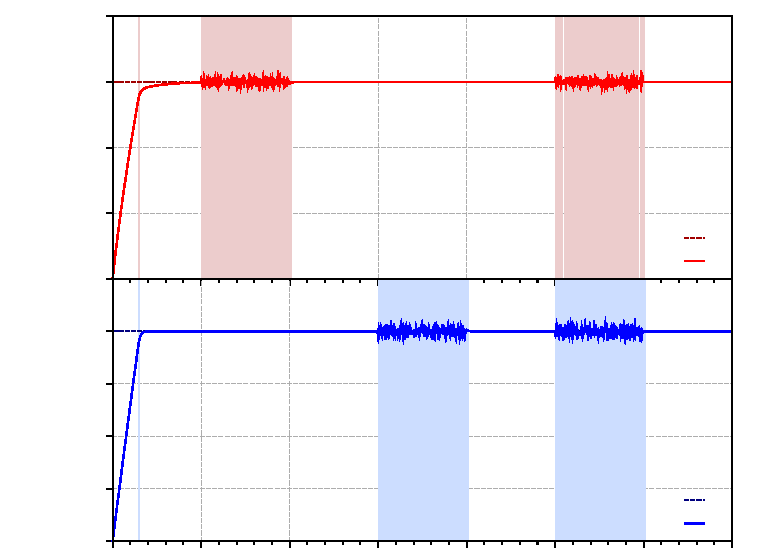
\includegraphics{fsesr}}%
    \gplfronttext
  \end{picture}%
\endgroup

\vspace{1cm}
\caption{FSeSR ($\pm 2\%$)}
\label{fig:fsesr}
\end{figure}

\begin{figure}[htb]
\footnotesize
\centering
% GNUPLOT: LaTeX picture with Postscript
\begingroup
  \makeatletter
  \providecommand\color[2][]{%
    \GenericError{(gnuplot) \space\space\space\@spaces}{%
      Package color not loaded in conjunction with
      terminal option `colourtext'%
    }{See the gnuplot documentation for explanation.%
    }{Either use 'blacktext' in gnuplot or load the package
      color.sty in LaTeX.}%
    \renewcommand\color[2][]{}%
  }%
  \providecommand\includegraphics[2][]{%
    \GenericError{(gnuplot) \space\space\space\@spaces}{%
      Package graphicx or graphics not loaded%
    }{See the gnuplot documentation for explanation.%
    }{The gnuplot epslatex terminal needs graphicx.sty or graphics.sty.}%
    \renewcommand\includegraphics[2][]{}%
  }%
  \providecommand\rotatebox[2]{#2}%
  \@ifundefined{ifGPcolor}{%
    \newif\ifGPcolor
    \GPcolortrue
  }{}%
  \@ifundefined{ifGPblacktext}{%
    \newif\ifGPblacktext
    \GPblacktexttrue
  }{}%
  % define a \g@addto@macro without @ in the name:
  \let\gplgaddtomacro\g@addto@macro
  % define empty templates for all commands taking text:
  \gdef\gplbacktext{}%
  \gdef\gplfronttext{}%
  \makeatother
  \ifGPblacktext
    % no textcolor at all
    \def\colorrgb#1{}%
    \def\colorgray#1{}%
  \else
    % gray or color?
    \ifGPcolor
      \def\colorrgb#1{\color[rgb]{#1}}%
      \def\colorgray#1{\color[gray]{#1}}%
      \expandafter\def\csname LTw\endcsname{\color{white}}%
      \expandafter\def\csname LTb\endcsname{\color{black}}%
      \expandafter\def\csname LTa\endcsname{\color{black}}%
      \expandafter\def\csname LT0\endcsname{\color[rgb]{1,0,0}}%
      \expandafter\def\csname LT1\endcsname{\color[rgb]{0,1,0}}%
      \expandafter\def\csname LT2\endcsname{\color[rgb]{0,0,1}}%
      \expandafter\def\csname LT3\endcsname{\color[rgb]{1,0,1}}%
      \expandafter\def\csname LT4\endcsname{\color[rgb]{0,1,1}}%
      \expandafter\def\csname LT5\endcsname{\color[rgb]{1,1,0}}%
      \expandafter\def\csname LT6\endcsname{\color[rgb]{0,0,0}}%
      \expandafter\def\csname LT7\endcsname{\color[rgb]{1,0.3,0}}%
      \expandafter\def\csname LT8\endcsname{\color[rgb]{0.5,0.5,0.5}}%
    \else
      % gray
      \def\colorrgb#1{\color{black}}%
      \def\colorgray#1{\color[gray]{#1}}%
      \expandafter\def\csname LTw\endcsname{\color{white}}%
      \expandafter\def\csname LTb\endcsname{\color{black}}%
      \expandafter\def\csname LTa\endcsname{\color{black}}%
      \expandafter\def\csname LT0\endcsname{\color{black}}%
      \expandafter\def\csname LT1\endcsname{\color{black}}%
      \expandafter\def\csname LT2\endcsname{\color{black}}%
      \expandafter\def\csname LT3\endcsname{\color{black}}%
      \expandafter\def\csname LT4\endcsname{\color{black}}%
      \expandafter\def\csname LT5\endcsname{\color{black}}%
      \expandafter\def\csname LT6\endcsname{\color{black}}%
      \expandafter\def\csname LT7\endcsname{\color{black}}%
      \expandafter\def\csname LT8\endcsname{\color{black}}%
    \fi
  \fi
  \setlength{\unitlength}{0.0500bp}%
  \begin{picture}(7200.00,5040.00)%
    \gplgaddtomacro\gplbacktext{%
      \csname LTb\endcsname%
      \put(726,2800){\makebox(0,0)[r]{\strut{} 5}}%
      \csname LTb\endcsname%
      \put(726,3080){\makebox(0,0)[r]{\strut{} 10}}%
      \csname LTb\endcsname%
      \put(726,3360){\makebox(0,0)[r]{\strut{} 15}}%
      \csname LTb\endcsname%
      \put(726,3640){\makebox(0,0)[r]{\strut{} 20}}%
      \csname LTb\endcsname%
      \put(726,3919){\makebox(0,0)[r]{\strut{} 25}}%
      \csname LTb\endcsname%
      \put(726,4199){\makebox(0,0)[r]{\strut{} 30}}%
      \csname LTb\endcsname%
      \put(726,4479){\makebox(0,0)[r]{\strut{} 35}}%
      \csname LTb\endcsname%
      \put(726,4759){\makebox(0,0)[r]{\strut{} 40}}%
      \csname LTb\endcsname%
      \put(726,5039){\makebox(0,0)[r]{\strut{} 45}}%
      \csname LTb\endcsname%
      \put(921,2237){\makebox(0,0){\strut{}}}%
      \csname LTb\endcsname%
      \put(1771,2237){\makebox(0,0){\strut{}}}%
      \csname LTb\endcsname%
      \put(2620,2237){\makebox(0,0){\strut{}}}%
      \csname LTb\endcsname%
      \put(3470,2237){\makebox(0,0){\strut{}}}%
      \csname LTb\endcsname%
      \put(4320,2237){\makebox(0,0){\strut{}}}%
      \csname LTb\endcsname%
      \put(5170,2237){\makebox(0,0){\strut{}}}%
      \csname LTb\endcsname%
      \put(6019,2237){\makebox(0,0){\strut{}}}%
      \csname LTb\endcsname%
      \put(6869,2237){\makebox(0,0){\strut{}}}%
      \put(352,3779){\rotatebox{-270}{\makebox(0,0){\strut{}Level [cm]}}}%
    }%
    \gplgaddtomacro\gplfronttext{%
      \csname LTb\endcsname%
      \put(6278,2913){\makebox(0,0)[r]{\strut{}Setpoint $T_1$}}%
      \csname LTb\endcsname%
      \put(6278,2693){\makebox(0,0)[r]{\strut{}Output $T_1$}}%
    }%
    \gplgaddtomacro\gplbacktext{%
      \csname LTb\endcsname%
      \put(726,0){\makebox(0,0)[r]{\strut{} 0}}%
      \csname LTb\endcsname%
      \put(726,315){\makebox(0,0)[r]{\strut{} 10}}%
      \csname LTb\endcsname%
      \put(726,630){\makebox(0,0)[r]{\strut{} 20}}%
      \csname LTb\endcsname%
      \put(726,945){\makebox(0,0)[r]{\strut{} 30}}%
      \csname LTb\endcsname%
      \put(726,1260){\makebox(0,0)[r]{\strut{} 40}}%
      \csname LTb\endcsname%
      \put(726,1575){\makebox(0,0)[r]{\strut{} 50}}%
      \csname LTb\endcsname%
      \put(726,1890){\makebox(0,0)[r]{\strut{} 60}}%
      \csname LTb\endcsname%
      \put(726,2205){\makebox(0,0)[r]{\strut{} 70}}%
      \csname LTb\endcsname%
      \put(726,2520){\makebox(0,0)[r]{\strut{} 80}}%
      \csname LTb\endcsname%
      \put(921,-283){\makebox(0,0){\strut{}0}}%
      \csname LTb\endcsname%
      \put(1771,-283){\makebox(0,0){\strut{}15}}%
      \csname LTb\endcsname%
      \put(2620,-283){\makebox(0,0){\strut{}30}}%
      \csname LTb\endcsname%
      \put(3470,-283){\makebox(0,0){\strut{}45}}%
      \csname LTb\endcsname%
      \put(4320,-283){\makebox(0,0){\strut{}60}}%
      \csname LTb\endcsname%
      \put(5170,-283){\makebox(0,0){\strut{}75}}%
      \csname LTb\endcsname%
      \put(6019,-283){\makebox(0,0){\strut{}90}}%
      \csname LTb\endcsname%
      \put(6869,-283){\makebox(0,0){\strut{}105}}%
      \put(352,1260){\rotatebox{-270}{\makebox(0,0){\strut{}Level [cm]}}}%
      \put(3895,-613){\makebox(0,0){\strut{}Time [s]}}%
    }%
    \gplgaddtomacro\gplfronttext{%
      \csname LTb\endcsname%
      \put(6278,393){\makebox(0,0)[r]{\strut{}Setpoint $T_2$}}%
      \csname LTb\endcsname%
      \put(6278,173){\makebox(0,0)[r]{\strut{}Output $T_2$}}%
    }%
    \gplbacktext
    \put(0,0){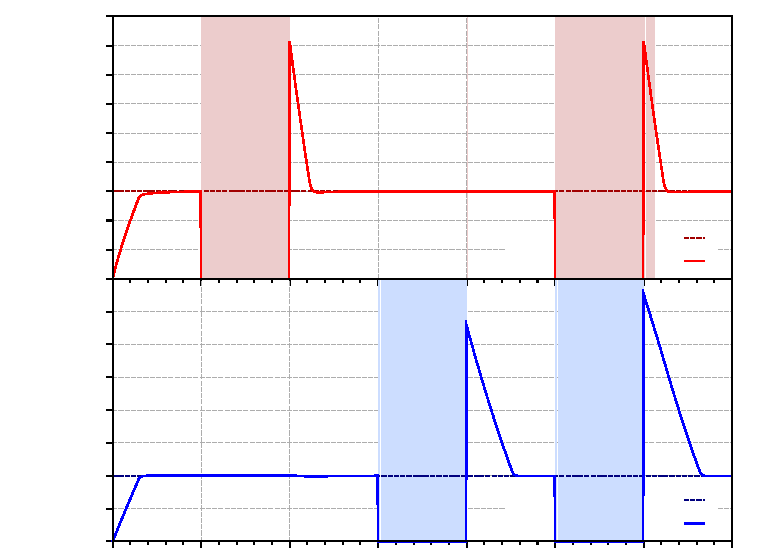
\includegraphics{fseq}}%
    \gplfronttext
  \end{picture}%
\endgroup

\vspace{1cm}
\caption{FSeQ (Ganho = 0)}
\label{fig:fseq}
\end{figure}

% Falhas nos atuadores .........................................................
\begin{figure}[htb]
\footnotesize
\centering
% GNUPLOT: LaTeX picture with Postscript
\begingroup
  \makeatletter
  \providecommand\color[2][]{%
    \GenericError{(gnuplot) \space\space\space\@spaces}{%
      Package color not loaded in conjunction with
      terminal option `colourtext'%
    }{See the gnuplot documentation for explanation.%
    }{Either use 'blacktext' in gnuplot or load the package
      color.sty in LaTeX.}%
    \renewcommand\color[2][]{}%
  }%
  \providecommand\includegraphics[2][]{%
    \GenericError{(gnuplot) \space\space\space\@spaces}{%
      Package graphicx or graphics not loaded%
    }{See the gnuplot documentation for explanation.%
    }{The gnuplot epslatex terminal needs graphicx.sty or graphics.sty.}%
    \renewcommand\includegraphics[2][]{}%
  }%
  \providecommand\rotatebox[2]{#2}%
  \@ifundefined{ifGPcolor}{%
    \newif\ifGPcolor
    \GPcolortrue
  }{}%
  \@ifundefined{ifGPblacktext}{%
    \newif\ifGPblacktext
    \GPblacktexttrue
  }{}%
  % define a \g@addto@macro without @ in the name:
  \let\gplgaddtomacro\g@addto@macro
  % define empty templates for all commands taking text:
  \gdef\gplbacktext{}%
  \gdef\gplfronttext{}%
  \makeatother
  \ifGPblacktext
    % no textcolor at all
    \def\colorrgb#1{}%
    \def\colorgray#1{}%
  \else
    % gray or color?
    \ifGPcolor
      \def\colorrgb#1{\color[rgb]{#1}}%
      \def\colorgray#1{\color[gray]{#1}}%
      \expandafter\def\csname LTw\endcsname{\color{white}}%
      \expandafter\def\csname LTb\endcsname{\color{black}}%
      \expandafter\def\csname LTa\endcsname{\color{black}}%
      \expandafter\def\csname LT0\endcsname{\color[rgb]{1,0,0}}%
      \expandafter\def\csname LT1\endcsname{\color[rgb]{0,1,0}}%
      \expandafter\def\csname LT2\endcsname{\color[rgb]{0,0,1}}%
      \expandafter\def\csname LT3\endcsname{\color[rgb]{1,0,1}}%
      \expandafter\def\csname LT4\endcsname{\color[rgb]{0,1,1}}%
      \expandafter\def\csname LT5\endcsname{\color[rgb]{1,1,0}}%
      \expandafter\def\csname LT6\endcsname{\color[rgb]{0,0,0}}%
      \expandafter\def\csname LT7\endcsname{\color[rgb]{1,0.3,0}}%
      \expandafter\def\csname LT8\endcsname{\color[rgb]{0.5,0.5,0.5}}%
    \else
      % gray
      \def\colorrgb#1{\color{black}}%
      \def\colorgray#1{\color[gray]{#1}}%
      \expandafter\def\csname LTw\endcsname{\color{white}}%
      \expandafter\def\csname LTb\endcsname{\color{black}}%
      \expandafter\def\csname LTa\endcsname{\color{black}}%
      \expandafter\def\csname LT0\endcsname{\color{black}}%
      \expandafter\def\csname LT1\endcsname{\color{black}}%
      \expandafter\def\csname LT2\endcsname{\color{black}}%
      \expandafter\def\csname LT3\endcsname{\color{black}}%
      \expandafter\def\csname LT4\endcsname{\color{black}}%
      \expandafter\def\csname LT5\endcsname{\color{black}}%
      \expandafter\def\csname LT6\endcsname{\color{black}}%
      \expandafter\def\csname LT7\endcsname{\color{black}}%
      \expandafter\def\csname LT8\endcsname{\color{black}}%
    \fi
  \fi
  \setlength{\unitlength}{0.0500bp}%
  \begin{picture}(7200.00,5040.00)%
    \gplgaddtomacro\gplbacktext{%
      \csname LTb\endcsname%
      \put(726,3150){\makebox(0,0)[r]{\strut{} 5}}%
      \csname LTb\endcsname%
      \put(726,3780){\makebox(0,0)[r]{\strut{} 10}}%
      \csname LTb\endcsname%
      \put(726,4409){\makebox(0,0)[r]{\strut{} 15}}%
      \csname LTb\endcsname%
      \put(726,5039){\makebox(0,0)[r]{\strut{} 20}}%
      \csname LTb\endcsname%
      \put(921,2237){\makebox(0,0){\strut{}}}%
      \csname LTb\endcsname%
      \put(1771,2237){\makebox(0,0){\strut{}}}%
      \csname LTb\endcsname%
      \put(2620,2237){\makebox(0,0){\strut{}}}%
      \csname LTb\endcsname%
      \put(3470,2237){\makebox(0,0){\strut{}}}%
      \csname LTb\endcsname%
      \put(4320,2237){\makebox(0,0){\strut{}}}%
      \csname LTb\endcsname%
      \put(5170,2237){\makebox(0,0){\strut{}}}%
      \csname LTb\endcsname%
      \put(6019,2237){\makebox(0,0){\strut{}}}%
      \csname LTb\endcsname%
      \put(6869,2237){\makebox(0,0){\strut{}}}%
      \put(352,3779){\rotatebox{-270}{\makebox(0,0){\strut{}Nível [cm]}}}%
    }%
    \gplgaddtomacro\gplfronttext{%
      \csname LTb\endcsname%
      \put(6278,2913){\makebox(0,0)[r]{\strut{}Ref. $T_1$}}%
      \csname LTb\endcsname%
      \put(6278,2693){\makebox(0,0)[r]{\strut{}Saída $T_1$}}%
    }%
    \gplgaddtomacro\gplbacktext{%
      \csname LTb\endcsname%
      \put(726,0){\makebox(0,0)[r]{\strut{} 0}}%
      \csname LTb\endcsname%
      \put(726,840){\makebox(0,0)[r]{\strut{} 10}}%
      \csname LTb\endcsname%
      \put(726,1680){\makebox(0,0)[r]{\strut{} 20}}%
      \csname LTb\endcsname%
      \put(726,2520){\makebox(0,0)[r]{\strut{} 30}}%
      \csname LTb\endcsname%
      \put(921,-283){\makebox(0,0){\strut{}0}}%
      \csname LTb\endcsname%
      \put(1771,-283){\makebox(0,0){\strut{}15}}%
      \csname LTb\endcsname%
      \put(2620,-283){\makebox(0,0){\strut{}30}}%
      \csname LTb\endcsname%
      \put(3470,-283){\makebox(0,0){\strut{}45}}%
      \csname LTb\endcsname%
      \put(4320,-283){\makebox(0,0){\strut{}60}}%
      \csname LTb\endcsname%
      \put(5170,-283){\makebox(0,0){\strut{}75}}%
      \csname LTb\endcsname%
      \put(6019,-283){\makebox(0,0){\strut{}90}}%
      \csname LTb\endcsname%
      \put(6869,-283){\makebox(0,0){\strut{}105}}%
      \put(352,1260){\rotatebox{-270}{\makebox(0,0){\strut{}Nível [cm]}}}%
      \put(3895,-613){\makebox(0,0){\strut{}Tempo [s]}}%
    }%
    \gplgaddtomacro\gplfronttext{%
      \csname LTb\endcsname%
      \put(6278,393){\makebox(0,0)[r]{\strut{}Ref. $T_2$}}%
      \csname LTb\endcsname%
      \put(6278,173){\makebox(0,0)[r]{\strut{}Saída $T_2$}}%
    }%
    \gplbacktext
    \put(0,0){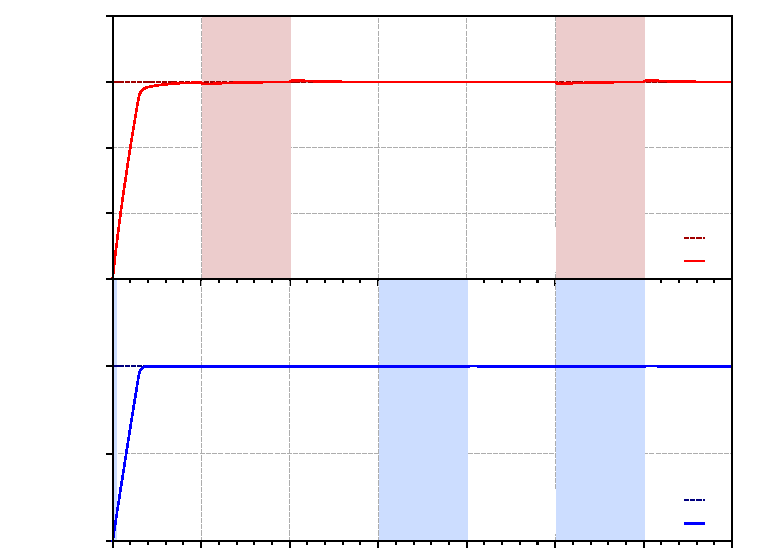
\includegraphics{fadg}}%
    \gplfronttext
  \end{picture}%
\endgroup

\vspace{1cm}
\caption{FADG (80\%)}
\label{fig:fadg}
\end{figure}

\begin{figure}[htb]
\footnotesize
\centering
% GNUPLOT: LaTeX picture with Postscript
\begingroup
  \makeatletter
  \providecommand\color[2][]{%
    \GenericError{(gnuplot) \space\space\space\@spaces}{%
      Package color not loaded in conjunction with
      terminal option `colourtext'%
    }{See the gnuplot documentation for explanation.%
    }{Either use 'blacktext' in gnuplot or load the package
      color.sty in LaTeX.}%
    \renewcommand\color[2][]{}%
  }%
  \providecommand\includegraphics[2][]{%
    \GenericError{(gnuplot) \space\space\space\@spaces}{%
      Package graphicx or graphics not loaded%
    }{See the gnuplot documentation for explanation.%
    }{The gnuplot epslatex terminal needs graphicx.sty or graphics.sty.}%
    \renewcommand\includegraphics[2][]{}%
  }%
  \providecommand\rotatebox[2]{#2}%
  \@ifundefined{ifGPcolor}{%
    \newif\ifGPcolor
    \GPcolortrue
  }{}%
  \@ifundefined{ifGPblacktext}{%
    \newif\ifGPblacktext
    \GPblacktexttrue
  }{}%
  % define a \g@addto@macro without @ in the name:
  \let\gplgaddtomacro\g@addto@macro
  % define empty templates for all commands taking text:
  \gdef\gplbacktext{}%
  \gdef\gplfronttext{}%
  \makeatother
  \ifGPblacktext
    % no textcolor at all
    \def\colorrgb#1{}%
    \def\colorgray#1{}%
  \else
    % gray or color?
    \ifGPcolor
      \def\colorrgb#1{\color[rgb]{#1}}%
      \def\colorgray#1{\color[gray]{#1}}%
      \expandafter\def\csname LTw\endcsname{\color{white}}%
      \expandafter\def\csname LTb\endcsname{\color{black}}%
      \expandafter\def\csname LTa\endcsname{\color{black}}%
      \expandafter\def\csname LT0\endcsname{\color[rgb]{1,0,0}}%
      \expandafter\def\csname LT1\endcsname{\color[rgb]{0,1,0}}%
      \expandafter\def\csname LT2\endcsname{\color[rgb]{0,0,1}}%
      \expandafter\def\csname LT3\endcsname{\color[rgb]{1,0,1}}%
      \expandafter\def\csname LT4\endcsname{\color[rgb]{0,1,1}}%
      \expandafter\def\csname LT5\endcsname{\color[rgb]{1,1,0}}%
      \expandafter\def\csname LT6\endcsname{\color[rgb]{0,0,0}}%
      \expandafter\def\csname LT7\endcsname{\color[rgb]{1,0.3,0}}%
      \expandafter\def\csname LT8\endcsname{\color[rgb]{0.5,0.5,0.5}}%
    \else
      % gray
      \def\colorrgb#1{\color{black}}%
      \def\colorgray#1{\color[gray]{#1}}%
      \expandafter\def\csname LTw\endcsname{\color{white}}%
      \expandafter\def\csname LTb\endcsname{\color{black}}%
      \expandafter\def\csname LTa\endcsname{\color{black}}%
      \expandafter\def\csname LT0\endcsname{\color{black}}%
      \expandafter\def\csname LT1\endcsname{\color{black}}%
      \expandafter\def\csname LT2\endcsname{\color{black}}%
      \expandafter\def\csname LT3\endcsname{\color{black}}%
      \expandafter\def\csname LT4\endcsname{\color{black}}%
      \expandafter\def\csname LT5\endcsname{\color{black}}%
      \expandafter\def\csname LT6\endcsname{\color{black}}%
      \expandafter\def\csname LT7\endcsname{\color{black}}%
      \expandafter\def\csname LT8\endcsname{\color{black}}%
    \fi
  \fi
  \setlength{\unitlength}{0.0500bp}%
  \begin{picture}(7200.00,5040.00)%
    \gplgaddtomacro\gplbacktext{%
      \csname LTb\endcsname%
      \put(726,3150){\makebox(0,0)[r]{\strut{} 5}}%
      \csname LTb\endcsname%
      \put(726,3780){\makebox(0,0)[r]{\strut{} 10}}%
      \csname LTb\endcsname%
      \put(726,4409){\makebox(0,0)[r]{\strut{} 15}}%
      \csname LTb\endcsname%
      \put(726,5039){\makebox(0,0)[r]{\strut{} 20}}%
      \csname LTb\endcsname%
      \put(921,2237){\makebox(0,0){\strut{}}}%
      \csname LTb\endcsname%
      \put(1771,2237){\makebox(0,0){\strut{}}}%
      \csname LTb\endcsname%
      \put(2620,2237){\makebox(0,0){\strut{}}}%
      \csname LTb\endcsname%
      \put(3470,2237){\makebox(0,0){\strut{}}}%
      \csname LTb\endcsname%
      \put(4320,2237){\makebox(0,0){\strut{}}}%
      \csname LTb\endcsname%
      \put(5170,2237){\makebox(0,0){\strut{}}}%
      \csname LTb\endcsname%
      \put(6019,2237){\makebox(0,0){\strut{}}}%
      \csname LTb\endcsname%
      \put(6869,2237){\makebox(0,0){\strut{}}}%
      \put(352,3779){\rotatebox{-270}{\makebox(0,0){\strut{}Level [cm]}}}%
    }%
    \gplgaddtomacro\gplfronttext{%
      \csname LTb\endcsname%
      \put(6278,2913){\makebox(0,0)[r]{\strut{}Setpoint $T_1$}}%
      \csname LTb\endcsname%
      \put(6278,2693){\makebox(0,0)[r]{\strut{}Output $T_1$}}%
    }%
    \gplgaddtomacro\gplbacktext{%
      \csname LTb\endcsname%
      \put(726,0){\makebox(0,0)[r]{\strut{} 0}}%
      \csname LTb\endcsname%
      \put(726,840){\makebox(0,0)[r]{\strut{} 10}}%
      \csname LTb\endcsname%
      \put(726,1680){\makebox(0,0)[r]{\strut{} 20}}%
      \csname LTb\endcsname%
      \put(726,2520){\makebox(0,0)[r]{\strut{} 30}}%
      \csname LTb\endcsname%
      \put(921,-283){\makebox(0,0){\strut{}0}}%
      \csname LTb\endcsname%
      \put(1771,-283){\makebox(0,0){\strut{}15}}%
      \csname LTb\endcsname%
      \put(2620,-283){\makebox(0,0){\strut{}30}}%
      \csname LTb\endcsname%
      \put(3470,-283){\makebox(0,0){\strut{}45}}%
      \csname LTb\endcsname%
      \put(4320,-283){\makebox(0,0){\strut{}60}}%
      \csname LTb\endcsname%
      \put(5170,-283){\makebox(0,0){\strut{}75}}%
      \csname LTb\endcsname%
      \put(6019,-283){\makebox(0,0){\strut{}90}}%
      \csname LTb\endcsname%
      \put(6869,-283){\makebox(0,0){\strut{}105}}%
      \put(352,1260){\rotatebox{-270}{\makebox(0,0){\strut{}Level [cm]}}}%
      \put(3895,-613){\makebox(0,0){\strut{}Time [s]}}%
    }%
    \gplgaddtomacro\gplfronttext{%
      \csname LTb\endcsname%
      \put(6278,393){\makebox(0,0)[r]{\strut{}Setpoint $T_2$}}%
      \csname LTb\endcsname%
      \put(6278,173){\makebox(0,0)[r]{\strut{}Output $T_2$}}%
    }%
    \gplbacktext
    \put(0,0){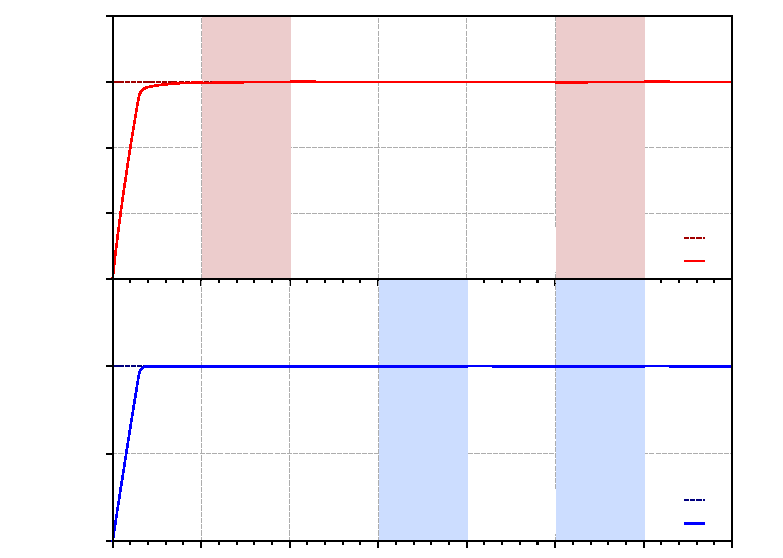
\includegraphics{fado}}%
    \gplfronttext
  \end{picture}%
\endgroup

\vspace{1cm}
\caption{FADO (-0,5 Volts)}
\label{fig:fado}
\end{figure}

\begin{figure}[htb]
\footnotesize
\centering
% GNUPLOT: LaTeX picture with Postscript
\begingroup
  \makeatletter
  \providecommand\color[2][]{%
    \GenericError{(gnuplot) \space\space\space\@spaces}{%
      Package color not loaded in conjunction with
      terminal option `colourtext'%
    }{See the gnuplot documentation for explanation.%
    }{Either use 'blacktext' in gnuplot or load the package
      color.sty in LaTeX.}%
    \renewcommand\color[2][]{}%
  }%
  \providecommand\includegraphics[2][]{%
    \GenericError{(gnuplot) \space\space\space\@spaces}{%
      Package graphicx or graphics not loaded%
    }{See the gnuplot documentation for explanation.%
    }{The gnuplot epslatex terminal needs graphicx.sty or graphics.sty.}%
    \renewcommand\includegraphics[2][]{}%
  }%
  \providecommand\rotatebox[2]{#2}%
  \@ifundefined{ifGPcolor}{%
    \newif\ifGPcolor
    \GPcolortrue
  }{}%
  \@ifundefined{ifGPblacktext}{%
    \newif\ifGPblacktext
    \GPblacktexttrue
  }{}%
  % define a \g@addto@macro without @ in the name:
  \let\gplgaddtomacro\g@addto@macro
  % define empty templates for all commands taking text:
  \gdef\gplbacktext{}%
  \gdef\gplfronttext{}%
  \makeatother
  \ifGPblacktext
    % no textcolor at all
    \def\colorrgb#1{}%
    \def\colorgray#1{}%
  \else
    % gray or color?
    \ifGPcolor
      \def\colorrgb#1{\color[rgb]{#1}}%
      \def\colorgray#1{\color[gray]{#1}}%
      \expandafter\def\csname LTw\endcsname{\color{white}}%
      \expandafter\def\csname LTb\endcsname{\color{black}}%
      \expandafter\def\csname LTa\endcsname{\color{black}}%
      \expandafter\def\csname LT0\endcsname{\color[rgb]{1,0,0}}%
      \expandafter\def\csname LT1\endcsname{\color[rgb]{0,1,0}}%
      \expandafter\def\csname LT2\endcsname{\color[rgb]{0,0,1}}%
      \expandafter\def\csname LT3\endcsname{\color[rgb]{1,0,1}}%
      \expandafter\def\csname LT4\endcsname{\color[rgb]{0,1,1}}%
      \expandafter\def\csname LT5\endcsname{\color[rgb]{1,1,0}}%
      \expandafter\def\csname LT6\endcsname{\color[rgb]{0,0,0}}%
      \expandafter\def\csname LT7\endcsname{\color[rgb]{1,0.3,0}}%
      \expandafter\def\csname LT8\endcsname{\color[rgb]{0.5,0.5,0.5}}%
    \else
      % gray
      \def\colorrgb#1{\color{black}}%
      \def\colorgray#1{\color[gray]{#1}}%
      \expandafter\def\csname LTw\endcsname{\color{white}}%
      \expandafter\def\csname LTb\endcsname{\color{black}}%
      \expandafter\def\csname LTa\endcsname{\color{black}}%
      \expandafter\def\csname LT0\endcsname{\color{black}}%
      \expandafter\def\csname LT1\endcsname{\color{black}}%
      \expandafter\def\csname LT2\endcsname{\color{black}}%
      \expandafter\def\csname LT3\endcsname{\color{black}}%
      \expandafter\def\csname LT4\endcsname{\color{black}}%
      \expandafter\def\csname LT5\endcsname{\color{black}}%
      \expandafter\def\csname LT6\endcsname{\color{black}}%
      \expandafter\def\csname LT7\endcsname{\color{black}}%
      \expandafter\def\csname LT8\endcsname{\color{black}}%
    \fi
  \fi
  \setlength{\unitlength}{0.0500bp}%
  \begin{picture}(7200.00,5040.00)%
    \gplgaddtomacro\gplbacktext{%
      \csname LTb\endcsname%
      \put(726,3150){\makebox(0,0)[r]{\strut{} 5}}%
      \csname LTb\endcsname%
      \put(726,3780){\makebox(0,0)[r]{\strut{} 10}}%
      \csname LTb\endcsname%
      \put(726,4409){\makebox(0,0)[r]{\strut{} 15}}%
      \csname LTb\endcsname%
      \put(726,5039){\makebox(0,0)[r]{\strut{} 20}}%
      \csname LTb\endcsname%
      \put(921,2237){\makebox(0,0){\strut{}}}%
      \csname LTb\endcsname%
      \put(1771,2237){\makebox(0,0){\strut{}}}%
      \csname LTb\endcsname%
      \put(2620,2237){\makebox(0,0){\strut{}}}%
      \csname LTb\endcsname%
      \put(3470,2237){\makebox(0,0){\strut{}}}%
      \csname LTb\endcsname%
      \put(4320,2237){\makebox(0,0){\strut{}}}%
      \csname LTb\endcsname%
      \put(5170,2237){\makebox(0,0){\strut{}}}%
      \csname LTb\endcsname%
      \put(6019,2237){\makebox(0,0){\strut{}}}%
      \csname LTb\endcsname%
      \put(6869,2237){\makebox(0,0){\strut{}}}%
      \put(352,3779){\rotatebox{-270}{\makebox(0,0){\strut{}Level [cm]}}}%
    }%
    \gplgaddtomacro\gplfronttext{%
      \csname LTb\endcsname%
      \put(6278,2913){\makebox(0,0)[r]{\strut{}Setpoint $T_1$}}%
      \csname LTb\endcsname%
      \put(6278,2693){\makebox(0,0)[r]{\strut{}Output $T_1$}}%
    }%
    \gplgaddtomacro\gplbacktext{%
      \csname LTb\endcsname%
      \put(726,0){\makebox(0,0)[r]{\strut{} 0}}%
      \csname LTb\endcsname%
      \put(726,840){\makebox(0,0)[r]{\strut{} 10}}%
      \csname LTb\endcsname%
      \put(726,1680){\makebox(0,0)[r]{\strut{} 20}}%
      \csname LTb\endcsname%
      \put(726,2520){\makebox(0,0)[r]{\strut{} 30}}%
      \csname LTb\endcsname%
      \put(921,-283){\makebox(0,0){\strut{}0}}%
      \csname LTb\endcsname%
      \put(1771,-283){\makebox(0,0){\strut{}15}}%
      \csname LTb\endcsname%
      \put(2620,-283){\makebox(0,0){\strut{}30}}%
      \csname LTb\endcsname%
      \put(3470,-283){\makebox(0,0){\strut{}45}}%
      \csname LTb\endcsname%
      \put(4320,-283){\makebox(0,0){\strut{}60}}%
      \csname LTb\endcsname%
      \put(5170,-283){\makebox(0,0){\strut{}75}}%
      \csname LTb\endcsname%
      \put(6019,-283){\makebox(0,0){\strut{}90}}%
      \csname LTb\endcsname%
      \put(6869,-283){\makebox(0,0){\strut{}105}}%
      \put(352,1260){\rotatebox{-270}{\makebox(0,0){\strut{}Level [cm]}}}%
      \put(3895,-613){\makebox(0,0){\strut{}Time [s]}}%
    }%
    \gplgaddtomacro\gplfronttext{%
      \csname LTb\endcsname%
      \put(6278,393){\makebox(0,0)[r]{\strut{}Setpoint $T_2$}}%
      \csname LTb\endcsname%
      \put(6278,173){\makebox(0,0)[r]{\strut{}Output $T_2$}}%
    }%
    \gplbacktext
    \put(0,0){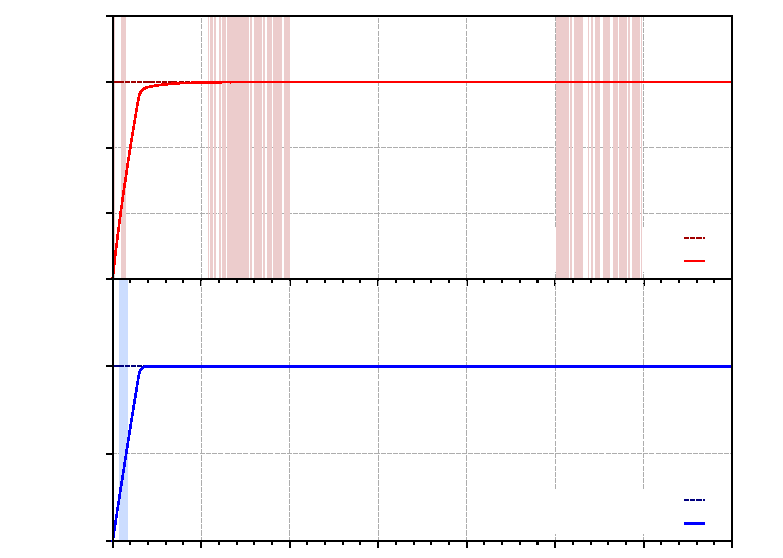
\includegraphics{fasr}}%
    \gplfronttext
  \end{picture}%
\endgroup

\vspace{1cm}
\caption{FASR ($\pm 2\%$)}
\label{fig:fasr}
\end{figure}

\begin{figure}[htb]
\footnotesize
\centering
% GNUPLOT: LaTeX picture with Postscript
\begingroup
  \makeatletter
  \providecommand\color[2][]{%
    \GenericError{(gnuplot) \space\space\space\@spaces}{%
      Package color not loaded in conjunction with
      terminal option `colourtext'%
    }{See the gnuplot documentation for explanation.%
    }{Either use 'blacktext' in gnuplot or load the package
      color.sty in LaTeX.}%
    \renewcommand\color[2][]{}%
  }%
  \providecommand\includegraphics[2][]{%
    \GenericError{(gnuplot) \space\space\space\@spaces}{%
      Package graphicx or graphics not loaded%
    }{See the gnuplot documentation for explanation.%
    }{The gnuplot epslatex terminal needs graphicx.sty or graphics.sty.}%
    \renewcommand\includegraphics[2][]{}%
  }%
  \providecommand\rotatebox[2]{#2}%
  \@ifundefined{ifGPcolor}{%
    \newif\ifGPcolor
    \GPcolortrue
  }{}%
  \@ifundefined{ifGPblacktext}{%
    \newif\ifGPblacktext
    \GPblacktexttrue
  }{}%
  % define a \g@addto@macro without @ in the name:
  \let\gplgaddtomacro\g@addto@macro
  % define empty templates for all commands taking text:
  \gdef\gplbacktext{}%
  \gdef\gplfronttext{}%
  \makeatother
  \ifGPblacktext
    % no textcolor at all
    \def\colorrgb#1{}%
    \def\colorgray#1{}%
  \else
    % gray or color?
    \ifGPcolor
      \def\colorrgb#1{\color[rgb]{#1}}%
      \def\colorgray#1{\color[gray]{#1}}%
      \expandafter\def\csname LTw\endcsname{\color{white}}%
      \expandafter\def\csname LTb\endcsname{\color{black}}%
      \expandafter\def\csname LTa\endcsname{\color{black}}%
      \expandafter\def\csname LT0\endcsname{\color[rgb]{1,0,0}}%
      \expandafter\def\csname LT1\endcsname{\color[rgb]{0,1,0}}%
      \expandafter\def\csname LT2\endcsname{\color[rgb]{0,0,1}}%
      \expandafter\def\csname LT3\endcsname{\color[rgb]{1,0,1}}%
      \expandafter\def\csname LT4\endcsname{\color[rgb]{0,1,1}}%
      \expandafter\def\csname LT5\endcsname{\color[rgb]{1,1,0}}%
      \expandafter\def\csname LT6\endcsname{\color[rgb]{0,0,0}}%
      \expandafter\def\csname LT7\endcsname{\color[rgb]{1,0.3,0}}%
      \expandafter\def\csname LT8\endcsname{\color[rgb]{0.5,0.5,0.5}}%
    \else
      % gray
      \def\colorrgb#1{\color{black}}%
      \def\colorgray#1{\color[gray]{#1}}%
      \expandafter\def\csname LTw\endcsname{\color{white}}%
      \expandafter\def\csname LTb\endcsname{\color{black}}%
      \expandafter\def\csname LTa\endcsname{\color{black}}%
      \expandafter\def\csname LT0\endcsname{\color{black}}%
      \expandafter\def\csname LT1\endcsname{\color{black}}%
      \expandafter\def\csname LT2\endcsname{\color{black}}%
      \expandafter\def\csname LT3\endcsname{\color{black}}%
      \expandafter\def\csname LT4\endcsname{\color{black}}%
      \expandafter\def\csname LT5\endcsname{\color{black}}%
      \expandafter\def\csname LT6\endcsname{\color{black}}%
      \expandafter\def\csname LT7\endcsname{\color{black}}%
      \expandafter\def\csname LT8\endcsname{\color{black}}%
    \fi
  \fi
  \setlength{\unitlength}{0.0500bp}%
  \begin{picture}(7200.00,5040.00)%
    \gplgaddtomacro\gplbacktext{%
      \csname LTb\endcsname%
      \put(726,3150){\makebox(0,0)[r]{\strut{} 5}}%
      \csname LTb\endcsname%
      \put(726,3780){\makebox(0,0)[r]{\strut{} 10}}%
      \csname LTb\endcsname%
      \put(726,4409){\makebox(0,0)[r]{\strut{} 15}}%
      \csname LTb\endcsname%
      \put(726,5039){\makebox(0,0)[r]{\strut{} 20}}%
      \csname LTb\endcsname%
      \put(921,2237){\makebox(0,0){\strut{}}}%
      \csname LTb\endcsname%
      \put(1771,2237){\makebox(0,0){\strut{}}}%
      \csname LTb\endcsname%
      \put(2620,2237){\makebox(0,0){\strut{}}}%
      \csname LTb\endcsname%
      \put(3470,2237){\makebox(0,0){\strut{}}}%
      \csname LTb\endcsname%
      \put(4320,2237){\makebox(0,0){\strut{}}}%
      \csname LTb\endcsname%
      \put(5170,2237){\makebox(0,0){\strut{}}}%
      \csname LTb\endcsname%
      \put(6019,2237){\makebox(0,0){\strut{}}}%
      \csname LTb\endcsname%
      \put(6869,2237){\makebox(0,0){\strut{}}}%
      \put(352,3779){\rotatebox{-270}{\makebox(0,0){\strut{}Nível [cm]}}}%
    }%
    \gplgaddtomacro\gplfronttext{%
      \csname LTb\endcsname%
      \put(6278,2913){\makebox(0,0)[r]{\strut{}Ref. $T_1$}}%
      \csname LTb\endcsname%
      \put(6278,2693){\makebox(0,0)[r]{\strut{}Saída $T_1$}}%
    }%
    \gplgaddtomacro\gplbacktext{%
      \csname LTb\endcsname%
      \put(726,0){\makebox(0,0)[r]{\strut{} 0}}%
      \csname LTb\endcsname%
      \put(726,840){\makebox(0,0)[r]{\strut{} 10}}%
      \csname LTb\endcsname%
      \put(726,1680){\makebox(0,0)[r]{\strut{} 20}}%
      \csname LTb\endcsname%
      \put(726,2520){\makebox(0,0)[r]{\strut{} 30}}%
      \csname LTb\endcsname%
      \put(921,-283){\makebox(0,0){\strut{}0}}%
      \csname LTb\endcsname%
      \put(1771,-283){\makebox(0,0){\strut{}15}}%
      \csname LTb\endcsname%
      \put(2620,-283){\makebox(0,0){\strut{}30}}%
      \csname LTb\endcsname%
      \put(3470,-283){\makebox(0,0){\strut{}45}}%
      \csname LTb\endcsname%
      \put(4320,-283){\makebox(0,0){\strut{}60}}%
      \csname LTb\endcsname%
      \put(5170,-283){\makebox(0,0){\strut{}75}}%
      \csname LTb\endcsname%
      \put(6019,-283){\makebox(0,0){\strut{}90}}%
      \csname LTb\endcsname%
      \put(6869,-283){\makebox(0,0){\strut{}105}}%
      \put(352,1260){\rotatebox{-270}{\makebox(0,0){\strut{}Nível [cm]}}}%
      \put(3895,-613){\makebox(0,0){\strut{}Tempo [s]}}%
    }%
    \gplgaddtomacro\gplfronttext{%
      \csname LTb\endcsname%
      \put(6278,393){\makebox(0,0)[r]{\strut{}Ref. $T_2$}}%
      \csname LTb\endcsname%
      \put(6278,173){\makebox(0,0)[r]{\strut{}Saída $T_2$}}%
    }%
    \gplbacktext
    \put(0,0){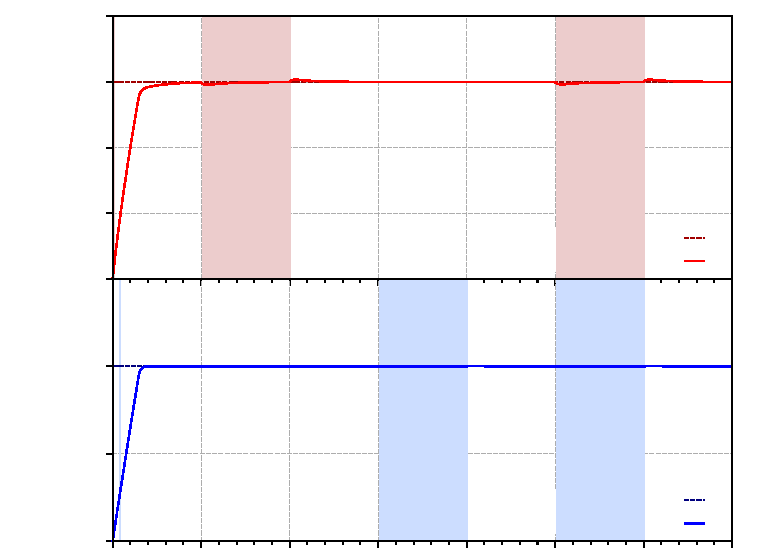
\includegraphics{favk}}%
    \gplfronttext
  \end{picture}%
\endgroup

\vspace{1cm}
\caption{FAVK (75\%)}
\label{fig:favk}
\end{figure}

\begin{figure}[htb]
\footnotesize
\centering
% GNUPLOT: LaTeX picture with Postscript
\begingroup
  \makeatletter
  \providecommand\color[2][]{%
    \GenericError{(gnuplot) \space\space\space\@spaces}{%
      Package color not loaded in conjunction with
      terminal option `colourtext'%
    }{See the gnuplot documentation for explanation.%
    }{Either use 'blacktext' in gnuplot or load the package
      color.sty in LaTeX.}%
    \renewcommand\color[2][]{}%
  }%
  \providecommand\includegraphics[2][]{%
    \GenericError{(gnuplot) \space\space\space\@spaces}{%
      Package graphicx or graphics not loaded%
    }{See the gnuplot documentation for explanation.%
    }{The gnuplot epslatex terminal needs graphicx.sty or graphics.sty.}%
    \renewcommand\includegraphics[2][]{}%
  }%
  \providecommand\rotatebox[2]{#2}%
  \@ifundefined{ifGPcolor}{%
    \newif\ifGPcolor
    \GPcolortrue
  }{}%
  \@ifundefined{ifGPblacktext}{%
    \newif\ifGPblacktext
    \GPblacktexttrue
  }{}%
  % define a \g@addto@macro without @ in the name:
  \let\gplgaddtomacro\g@addto@macro
  % define empty templates for all commands taking text:
  \gdef\gplbacktext{}%
  \gdef\gplfronttext{}%
  \makeatother
  \ifGPblacktext
    % no textcolor at all
    \def\colorrgb#1{}%
    \def\colorgray#1{}%
  \else
    % gray or color?
    \ifGPcolor
      \def\colorrgb#1{\color[rgb]{#1}}%
      \def\colorgray#1{\color[gray]{#1}}%
      \expandafter\def\csname LTw\endcsname{\color{white}}%
      \expandafter\def\csname LTb\endcsname{\color{black}}%
      \expandafter\def\csname LTa\endcsname{\color{black}}%
      \expandafter\def\csname LT0\endcsname{\color[rgb]{1,0,0}}%
      \expandafter\def\csname LT1\endcsname{\color[rgb]{0,1,0}}%
      \expandafter\def\csname LT2\endcsname{\color[rgb]{0,0,1}}%
      \expandafter\def\csname LT3\endcsname{\color[rgb]{1,0,1}}%
      \expandafter\def\csname LT4\endcsname{\color[rgb]{0,1,1}}%
      \expandafter\def\csname LT5\endcsname{\color[rgb]{1,1,0}}%
      \expandafter\def\csname LT6\endcsname{\color[rgb]{0,0,0}}%
      \expandafter\def\csname LT7\endcsname{\color[rgb]{1,0.3,0}}%
      \expandafter\def\csname LT8\endcsname{\color[rgb]{0.5,0.5,0.5}}%
    \else
      % gray
      \def\colorrgb#1{\color{black}}%
      \def\colorgray#1{\color[gray]{#1}}%
      \expandafter\def\csname LTw\endcsname{\color{white}}%
      \expandafter\def\csname LTb\endcsname{\color{black}}%
      \expandafter\def\csname LTa\endcsname{\color{black}}%
      \expandafter\def\csname LT0\endcsname{\color{black}}%
      \expandafter\def\csname LT1\endcsname{\color{black}}%
      \expandafter\def\csname LT2\endcsname{\color{black}}%
      \expandafter\def\csname LT3\endcsname{\color{black}}%
      \expandafter\def\csname LT4\endcsname{\color{black}}%
      \expandafter\def\csname LT5\endcsname{\color{black}}%
      \expandafter\def\csname LT6\endcsname{\color{black}}%
      \expandafter\def\csname LT7\endcsname{\color{black}}%
      \expandafter\def\csname LT8\endcsname{\color{black}}%
    \fi
  \fi
  \setlength{\unitlength}{0.0500bp}%
  \begin{picture}(7200.00,5040.00)%
    \gplgaddtomacro\gplbacktext{%
      \csname LTb\endcsname%
      \put(726,3150){\makebox(0,0)[r]{\strut{} 5}}%
      \csname LTb\endcsname%
      \put(726,3780){\makebox(0,0)[r]{\strut{} 10}}%
      \csname LTb\endcsname%
      \put(726,4409){\makebox(0,0)[r]{\strut{} 15}}%
      \csname LTb\endcsname%
      \put(726,5039){\makebox(0,0)[r]{\strut{} 20}}%
      \csname LTb\endcsname%
      \put(921,2237){\makebox(0,0){\strut{}}}%
      \csname LTb\endcsname%
      \put(1771,2237){\makebox(0,0){\strut{}}}%
      \csname LTb\endcsname%
      \put(2620,2237){\makebox(0,0){\strut{}}}%
      \csname LTb\endcsname%
      \put(3470,2237){\makebox(0,0){\strut{}}}%
      \csname LTb\endcsname%
      \put(4320,2237){\makebox(0,0){\strut{}}}%
      \csname LTb\endcsname%
      \put(5170,2237){\makebox(0,0){\strut{}}}%
      \csname LTb\endcsname%
      \put(6019,2237){\makebox(0,0){\strut{}}}%
      \csname LTb\endcsname%
      \put(6869,2237){\makebox(0,0){\strut{}}}%
      \put(352,3779){\rotatebox{-270}{\makebox(0,0){\strut{}Level [cm]}}}%
    }%
    \gplgaddtomacro\gplfronttext{%
      \csname LTb\endcsname%
      \put(6278,2913){\makebox(0,0)[r]{\strut{}Setpoint $T_1$}}%
      \csname LTb\endcsname%
      \put(6278,2693){\makebox(0,0)[r]{\strut{}Output $T_1$}}%
    }%
    \gplgaddtomacro\gplbacktext{%
      \csname LTb\endcsname%
      \put(726,0){\makebox(0,0)[r]{\strut{} 0}}%
      \csname LTb\endcsname%
      \put(726,840){\makebox(0,0)[r]{\strut{} 10}}%
      \csname LTb\endcsname%
      \put(726,1680){\makebox(0,0)[r]{\strut{} 20}}%
      \csname LTb\endcsname%
      \put(726,2520){\makebox(0,0)[r]{\strut{} 30}}%
      \csname LTb\endcsname%
      \put(921,-283){\makebox(0,0){\strut{}0}}%
      \csname LTb\endcsname%
      \put(1771,-283){\makebox(0,0){\strut{}15}}%
      \csname LTb\endcsname%
      \put(2620,-283){\makebox(0,0){\strut{}30}}%
      \csname LTb\endcsname%
      \put(3470,-283){\makebox(0,0){\strut{}45}}%
      \csname LTb\endcsname%
      \put(4320,-283){\makebox(0,0){\strut{}60}}%
      \csname LTb\endcsname%
      \put(5170,-283){\makebox(0,0){\strut{}75}}%
      \csname LTb\endcsname%
      \put(6019,-283){\makebox(0,0){\strut{}90}}%
      \csname LTb\endcsname%
      \put(6869,-283){\makebox(0,0){\strut{}105}}%
      \put(352,1260){\rotatebox{-270}{\makebox(0,0){\strut{}Level [cm]}}}%
      \put(3895,-613){\makebox(0,0){\strut{}Time [s]}}%
    }%
    \gplgaddtomacro\gplfronttext{%
      \csname LTb\endcsname%
      \put(6278,393){\makebox(0,0)[r]{\strut{}Setpoint $T_2$}}%
      \csname LTb\endcsname%
      \put(6278,173){\makebox(0,0)[r]{\strut{}Output $T_2$}}%
    }%
    \gplbacktext
    \put(0,0){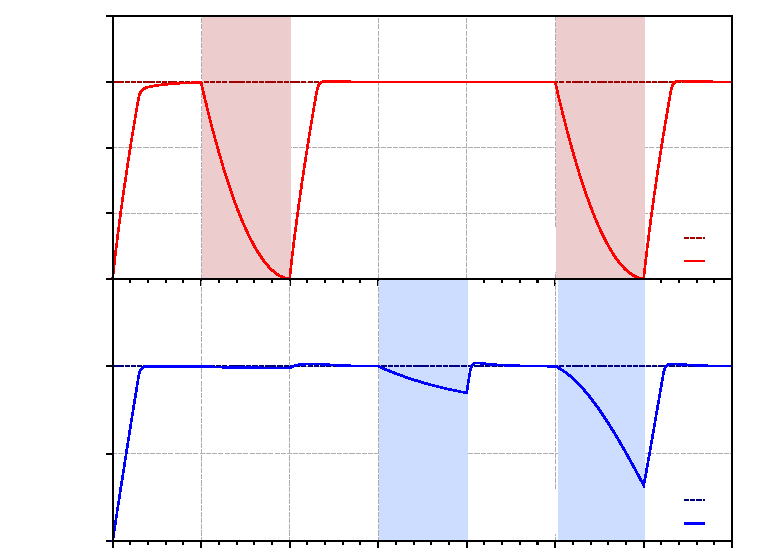
\includegraphics{faq}}%
    \gplfronttext
  \end{picture}%
\endgroup

\vspace{1cm}
\caption{FAQ (Ganho = 0)}
\label{fig:faq}
\end{figure}

% Falhas no sistema ............................................................
\begin{figure}[htb]
\footnotesize
\centering
% GNUPLOT: LaTeX picture with Postscript
\begingroup
  \makeatletter
  \providecommand\color[2][]{%
    \GenericError{(gnuplot) \space\space\space\@spaces}{%
      Package color not loaded in conjunction with
      terminal option `colourtext'%
    }{See the gnuplot documentation for explanation.%
    }{Either use 'blacktext' in gnuplot or load the package
      color.sty in LaTeX.}%
    \renewcommand\color[2][]{}%
  }%
  \providecommand\includegraphics[2][]{%
    \GenericError{(gnuplot) \space\space\space\@spaces}{%
      Package graphicx or graphics not loaded%
    }{See the gnuplot documentation for explanation.%
    }{The gnuplot epslatex terminal needs graphicx.sty or graphics.sty.}%
    \renewcommand\includegraphics[2][]{}%
  }%
  \providecommand\rotatebox[2]{#2}%
  \@ifundefined{ifGPcolor}{%
    \newif\ifGPcolor
    \GPcolortrue
  }{}%
  \@ifundefined{ifGPblacktext}{%
    \newif\ifGPblacktext
    \GPblacktexttrue
  }{}%
  % define a \g@addto@macro without @ in the name:
  \let\gplgaddtomacro\g@addto@macro
  % define empty templates for all commands taking text:
  \gdef\gplbacktext{}%
  \gdef\gplfronttext{}%
  \makeatother
  \ifGPblacktext
    % no textcolor at all
    \def\colorrgb#1{}%
    \def\colorgray#1{}%
  \else
    % gray or color?
    \ifGPcolor
      \def\colorrgb#1{\color[rgb]{#1}}%
      \def\colorgray#1{\color[gray]{#1}}%
      \expandafter\def\csname LTw\endcsname{\color{white}}%
      \expandafter\def\csname LTb\endcsname{\color{black}}%
      \expandafter\def\csname LTa\endcsname{\color{black}}%
      \expandafter\def\csname LT0\endcsname{\color[rgb]{1,0,0}}%
      \expandafter\def\csname LT1\endcsname{\color[rgb]{0,1,0}}%
      \expandafter\def\csname LT2\endcsname{\color[rgb]{0,0,1}}%
      \expandafter\def\csname LT3\endcsname{\color[rgb]{1,0,1}}%
      \expandafter\def\csname LT4\endcsname{\color[rgb]{0,1,1}}%
      \expandafter\def\csname LT5\endcsname{\color[rgb]{1,1,0}}%
      \expandafter\def\csname LT6\endcsname{\color[rgb]{0,0,0}}%
      \expandafter\def\csname LT7\endcsname{\color[rgb]{1,0.3,0}}%
      \expandafter\def\csname LT8\endcsname{\color[rgb]{0.5,0.5,0.5}}%
    \else
      % gray
      \def\colorrgb#1{\color{black}}%
      \def\colorgray#1{\color[gray]{#1}}%
      \expandafter\def\csname LTw\endcsname{\color{white}}%
      \expandafter\def\csname LTb\endcsname{\color{black}}%
      \expandafter\def\csname LTa\endcsname{\color{black}}%
      \expandafter\def\csname LT0\endcsname{\color{black}}%
      \expandafter\def\csname LT1\endcsname{\color{black}}%
      \expandafter\def\csname LT2\endcsname{\color{black}}%
      \expandafter\def\csname LT3\endcsname{\color{black}}%
      \expandafter\def\csname LT4\endcsname{\color{black}}%
      \expandafter\def\csname LT5\endcsname{\color{black}}%
      \expandafter\def\csname LT6\endcsname{\color{black}}%
      \expandafter\def\csname LT7\endcsname{\color{black}}%
      \expandafter\def\csname LT8\endcsname{\color{black}}%
    \fi
  \fi
  \setlength{\unitlength}{0.0500bp}%
  \begin{picture}(7200.00,5040.00)%
    \gplgaddtomacro\gplbacktext{%
      \csname LTb\endcsname%
      \put(726,3150){\makebox(0,0)[r]{\strut{} 5}}%
      \csname LTb\endcsname%
      \put(726,3780){\makebox(0,0)[r]{\strut{} 10}}%
      \csname LTb\endcsname%
      \put(726,4409){\makebox(0,0)[r]{\strut{} 15}}%
      \csname LTb\endcsname%
      \put(726,5039){\makebox(0,0)[r]{\strut{} 20}}%
      \csname LTb\endcsname%
      \put(921,2237){\makebox(0,0){\strut{}}}%
      \csname LTb\endcsname%
      \put(1771,2237){\makebox(0,0){\strut{}}}%
      \csname LTb\endcsname%
      \put(2620,2237){\makebox(0,0){\strut{}}}%
      \csname LTb\endcsname%
      \put(3470,2237){\makebox(0,0){\strut{}}}%
      \csname LTb\endcsname%
      \put(4320,2237){\makebox(0,0){\strut{}}}%
      \csname LTb\endcsname%
      \put(5170,2237){\makebox(0,0){\strut{}}}%
      \csname LTb\endcsname%
      \put(6019,2237){\makebox(0,0){\strut{}}}%
      \csname LTb\endcsname%
      \put(6869,2237){\makebox(0,0){\strut{}}}%
      \put(352,3779){\rotatebox{-270}{\makebox(0,0){\strut{}Nível [cm]}}}%
    }%
    \gplgaddtomacro\gplfronttext{%
      \csname LTb\endcsname%
      \put(6278,2913){\makebox(0,0)[r]{\strut{}Ref. $T_1$}}%
      \csname LTb\endcsname%
      \put(6278,2693){\makebox(0,0)[r]{\strut{}Saída $T_1$}}%
    }%
    \gplgaddtomacro\gplbacktext{%
      \csname LTb\endcsname%
      \put(726,0){\makebox(0,0)[r]{\strut{} 0}}%
      \csname LTb\endcsname%
      \put(726,840){\makebox(0,0)[r]{\strut{} 10}}%
      \csname LTb\endcsname%
      \put(726,1680){\makebox(0,0)[r]{\strut{} 20}}%
      \csname LTb\endcsname%
      \put(726,2520){\makebox(0,0)[r]{\strut{} 30}}%
      \csname LTb\endcsname%
      \put(921,-283){\makebox(0,0){\strut{}0}}%
      \csname LTb\endcsname%
      \put(1771,-283){\makebox(0,0){\strut{}15}}%
      \csname LTb\endcsname%
      \put(2620,-283){\makebox(0,0){\strut{}30}}%
      \csname LTb\endcsname%
      \put(3470,-283){\makebox(0,0){\strut{}45}}%
      \csname LTb\endcsname%
      \put(4320,-283){\makebox(0,0){\strut{}60}}%
      \csname LTb\endcsname%
      \put(5170,-283){\makebox(0,0){\strut{}75}}%
      \csname LTb\endcsname%
      \put(6019,-283){\makebox(0,0){\strut{}90}}%
      \csname LTb\endcsname%
      \put(6869,-283){\makebox(0,0){\strut{}105}}%
      \put(352,1260){\rotatebox{-270}{\makebox(0,0){\strut{}Nível [cm]}}}%
      \put(3895,-613){\makebox(0,0){\strut{}Tempo [s]}}%
    }%
    \gplgaddtomacro\gplfronttext{%
      \csname LTb\endcsname%
      \put(6278,393){\makebox(0,0)[r]{\strut{}Ref. $T_2$}}%
      \csname LTb\endcsname%
      \put(6278,173){\makebox(0,0)[r]{\strut{}Saída $T_2$}}%
    }%
    \gplbacktext
    \put(0,0){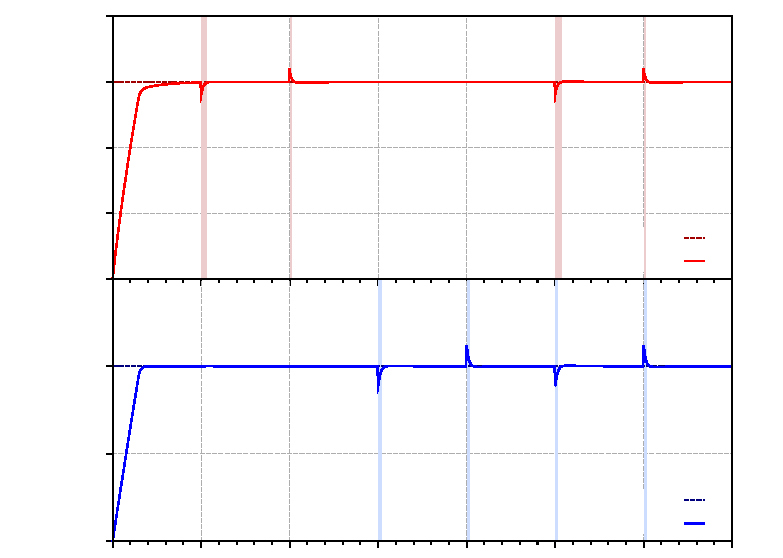
\includegraphics{fsivzt}}%
    \gplfronttext
  \end{picture}%
\endgroup

\vspace{1cm}
\caption{FSiVzT ($a_{\tiny VZ} = \frac{a_{\tiny MED}}{2}$)}
\label{fig:fsivzt}
\end{figure}

\begin{figure}[htb]
\footnotesize
\centering
% GNUPLOT: LaTeX picture with Postscript
\begingroup
  \makeatletter
  \providecommand\color[2][]{%
    \GenericError{(gnuplot) \space\space\space\@spaces}{%
      Package color not loaded in conjunction with
      terminal option `colourtext'%
    }{See the gnuplot documentation for explanation.%
    }{Either use 'blacktext' in gnuplot or load the package
      color.sty in LaTeX.}%
    \renewcommand\color[2][]{}%
  }%
  \providecommand\includegraphics[2][]{%
    \GenericError{(gnuplot) \space\space\space\@spaces}{%
      Package graphicx or graphics not loaded%
    }{See the gnuplot documentation for explanation.%
    }{The gnuplot epslatex terminal needs graphicx.sty or graphics.sty.}%
    \renewcommand\includegraphics[2][]{}%
  }%
  \providecommand\rotatebox[2]{#2}%
  \@ifundefined{ifGPcolor}{%
    \newif\ifGPcolor
    \GPcolortrue
  }{}%
  \@ifundefined{ifGPblacktext}{%
    \newif\ifGPblacktext
    \GPblacktexttrue
  }{}%
  % define a \g@addto@macro without @ in the name:
  \let\gplgaddtomacro\g@addto@macro
  % define empty templates for all commands taking text:
  \gdef\gplbacktext{}%
  \gdef\gplfronttext{}%
  \makeatother
  \ifGPblacktext
    % no textcolor at all
    \def\colorrgb#1{}%
    \def\colorgray#1{}%
  \else
    % gray or color?
    \ifGPcolor
      \def\colorrgb#1{\color[rgb]{#1}}%
      \def\colorgray#1{\color[gray]{#1}}%
      \expandafter\def\csname LTw\endcsname{\color{white}}%
      \expandafter\def\csname LTb\endcsname{\color{black}}%
      \expandafter\def\csname LTa\endcsname{\color{black}}%
      \expandafter\def\csname LT0\endcsname{\color[rgb]{1,0,0}}%
      \expandafter\def\csname LT1\endcsname{\color[rgb]{0,1,0}}%
      \expandafter\def\csname LT2\endcsname{\color[rgb]{0,0,1}}%
      \expandafter\def\csname LT3\endcsname{\color[rgb]{1,0,1}}%
      \expandafter\def\csname LT4\endcsname{\color[rgb]{0,1,1}}%
      \expandafter\def\csname LT5\endcsname{\color[rgb]{1,1,0}}%
      \expandafter\def\csname LT6\endcsname{\color[rgb]{0,0,0}}%
      \expandafter\def\csname LT7\endcsname{\color[rgb]{1,0.3,0}}%
      \expandafter\def\csname LT8\endcsname{\color[rgb]{0.5,0.5,0.5}}%
    \else
      % gray
      \def\colorrgb#1{\color{black}}%
      \def\colorgray#1{\color[gray]{#1}}%
      \expandafter\def\csname LTw\endcsname{\color{white}}%
      \expandafter\def\csname LTb\endcsname{\color{black}}%
      \expandafter\def\csname LTa\endcsname{\color{black}}%
      \expandafter\def\csname LT0\endcsname{\color{black}}%
      \expandafter\def\csname LT1\endcsname{\color{black}}%
      \expandafter\def\csname LT2\endcsname{\color{black}}%
      \expandafter\def\csname LT3\endcsname{\color{black}}%
      \expandafter\def\csname LT4\endcsname{\color{black}}%
      \expandafter\def\csname LT5\endcsname{\color{black}}%
      \expandafter\def\csname LT6\endcsname{\color{black}}%
      \expandafter\def\csname LT7\endcsname{\color{black}}%
      \expandafter\def\csname LT8\endcsname{\color{black}}%
    \fi
  \fi
  \setlength{\unitlength}{0.0500bp}%
  \begin{picture}(7200.00,5040.00)%
    \gplgaddtomacro\gplbacktext{%
      \csname LTb\endcsname%
      \put(726,3150){\makebox(0,0)[r]{\strut{} 5}}%
      \csname LTb\endcsname%
      \put(726,3780){\makebox(0,0)[r]{\strut{} 10}}%
      \csname LTb\endcsname%
      \put(726,4409){\makebox(0,0)[r]{\strut{} 15}}%
      \csname LTb\endcsname%
      \put(726,5039){\makebox(0,0)[r]{\strut{} 20}}%
      \csname LTb\endcsname%
      \put(921,2237){\makebox(0,0){\strut{}}}%
      \csname LTb\endcsname%
      \put(1771,2237){\makebox(0,0){\strut{}}}%
      \csname LTb\endcsname%
      \put(2620,2237){\makebox(0,0){\strut{}}}%
      \csname LTb\endcsname%
      \put(3470,2237){\makebox(0,0){\strut{}}}%
      \csname LTb\endcsname%
      \put(4320,2237){\makebox(0,0){\strut{}}}%
      \csname LTb\endcsname%
      \put(5170,2237){\makebox(0,0){\strut{}}}%
      \csname LTb\endcsname%
      \put(6019,2237){\makebox(0,0){\strut{}}}%
      \csname LTb\endcsname%
      \put(6869,2237){\makebox(0,0){\strut{}}}%
      \put(352,3779){\rotatebox{-270}{\makebox(0,0){\strut{}Nível [cm]}}}%
    }%
    \gplgaddtomacro\gplfronttext{%
      \csname LTb\endcsname%
      \put(6278,2913){\makebox(0,0)[r]{\strut{}Ref. $T_1$}}%
      \csname LTb\endcsname%
      \put(6278,2693){\makebox(0,0)[r]{\strut{}Saída $T_1$}}%
    }%
    \gplgaddtomacro\gplbacktext{%
      \csname LTb\endcsname%
      \put(726,0){\makebox(0,0)[r]{\strut{} 0}}%
      \csname LTb\endcsname%
      \put(726,840){\makebox(0,0)[r]{\strut{} 10}}%
      \csname LTb\endcsname%
      \put(726,1680){\makebox(0,0)[r]{\strut{} 20}}%
      \csname LTb\endcsname%
      \put(726,2520){\makebox(0,0)[r]{\strut{} 30}}%
      \csname LTb\endcsname%
      \put(921,-283){\makebox(0,0){\strut{}0}}%
      \csname LTb\endcsname%
      \put(1771,-283){\makebox(0,0){\strut{}15}}%
      \csname LTb\endcsname%
      \put(2620,-283){\makebox(0,0){\strut{}30}}%
      \csname LTb\endcsname%
      \put(3470,-283){\makebox(0,0){\strut{}45}}%
      \csname LTb\endcsname%
      \put(4320,-283){\makebox(0,0){\strut{}60}}%
      \csname LTb\endcsname%
      \put(5170,-283){\makebox(0,0){\strut{}75}}%
      \csname LTb\endcsname%
      \put(6019,-283){\makebox(0,0){\strut{}90}}%
      \csname LTb\endcsname%
      \put(6869,-283){\makebox(0,0){\strut{}105}}%
      \put(352,1260){\rotatebox{-270}{\makebox(0,0){\strut{}Nível [cm]}}}%
      \put(3895,-613){\makebox(0,0){\strut{}Tempo [s]}}%
    }%
    \gplgaddtomacro\gplfronttext{%
      \csname LTb\endcsname%
      \put(6278,393){\makebox(0,0)[r]{\strut{}Ref. $T_2$}}%
      \csname LTb\endcsname%
      \put(6278,173){\makebox(0,0)[r]{\strut{}Saída $T_2$}}%
    }%
    \gplbacktext
    \put(0,0){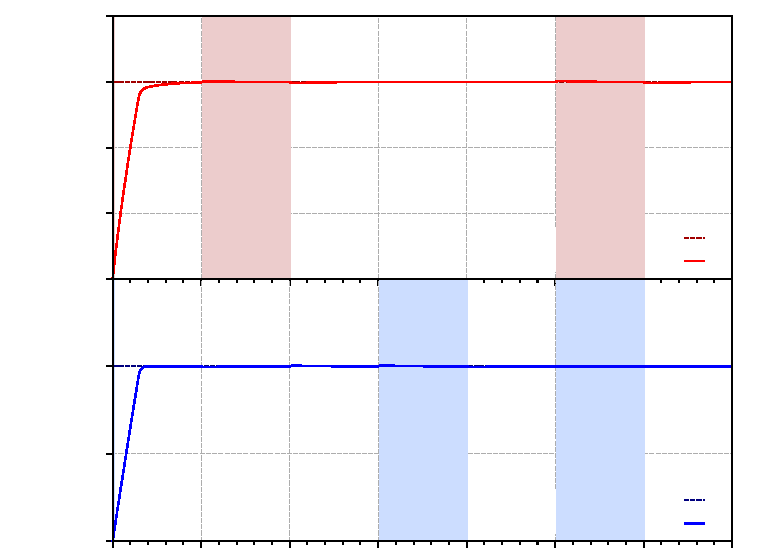
\includegraphics{fsivros}}%
    \gplfronttext
  \end{picture}%
\endgroup

\vspace{1cm}
\caption{FSiVrOS ($a' = \frac{a_{\tiny MED}}{2}$)}
\label{fig:fsivros}
\end{figure}

\begin{figure}[htb]
\footnotesize
\centering
% GNUPLOT: LaTeX picture with Postscript
\begingroup
  \makeatletter
  \providecommand\color[2][]{%
    \GenericError{(gnuplot) \space\space\space\@spaces}{%
      Package color not loaded in conjunction with
      terminal option `colourtext'%
    }{See the gnuplot documentation for explanation.%
    }{Either use 'blacktext' in gnuplot or load the package
      color.sty in LaTeX.}%
    \renewcommand\color[2][]{}%
  }%
  \providecommand\includegraphics[2][]{%
    \GenericError{(gnuplot) \space\space\space\@spaces}{%
      Package graphicx or graphics not loaded%
    }{See the gnuplot documentation for explanation.%
    }{The gnuplot epslatex terminal needs graphicx.sty or graphics.sty.}%
    \renewcommand\includegraphics[2][]{}%
  }%
  \providecommand\rotatebox[2]{#2}%
  \@ifundefined{ifGPcolor}{%
    \newif\ifGPcolor
    \GPcolortrue
  }{}%
  \@ifundefined{ifGPblacktext}{%
    \newif\ifGPblacktext
    \GPblacktexttrue
  }{}%
  % define a \g@addto@macro without @ in the name:
  \let\gplgaddtomacro\g@addto@macro
  % define empty templates for all commands taking text:
  \gdef\gplbacktext{}%
  \gdef\gplfronttext{}%
  \makeatother
  \ifGPblacktext
    % no textcolor at all
    \def\colorrgb#1{}%
    \def\colorgray#1{}%
  \else
    % gray or color?
    \ifGPcolor
      \def\colorrgb#1{\color[rgb]{#1}}%
      \def\colorgray#1{\color[gray]{#1}}%
      \expandafter\def\csname LTw\endcsname{\color{white}}%
      \expandafter\def\csname LTb\endcsname{\color{black}}%
      \expandafter\def\csname LTa\endcsname{\color{black}}%
      \expandafter\def\csname LT0\endcsname{\color[rgb]{1,0,0}}%
      \expandafter\def\csname LT1\endcsname{\color[rgb]{0,1,0}}%
      \expandafter\def\csname LT2\endcsname{\color[rgb]{0,0,1}}%
      \expandafter\def\csname LT3\endcsname{\color[rgb]{1,0,1}}%
      \expandafter\def\csname LT4\endcsname{\color[rgb]{0,1,1}}%
      \expandafter\def\csname LT5\endcsname{\color[rgb]{1,1,0}}%
      \expandafter\def\csname LT6\endcsname{\color[rgb]{0,0,0}}%
      \expandafter\def\csname LT7\endcsname{\color[rgb]{1,0.3,0}}%
      \expandafter\def\csname LT8\endcsname{\color[rgb]{0.5,0.5,0.5}}%
    \else
      % gray
      \def\colorrgb#1{\color{black}}%
      \def\colorgray#1{\color[gray]{#1}}%
      \expandafter\def\csname LTw\endcsname{\color{white}}%
      \expandafter\def\csname LTb\endcsname{\color{black}}%
      \expandafter\def\csname LTa\endcsname{\color{black}}%
      \expandafter\def\csname LT0\endcsname{\color{black}}%
      \expandafter\def\csname LT1\endcsname{\color{black}}%
      \expandafter\def\csname LT2\endcsname{\color{black}}%
      \expandafter\def\csname LT3\endcsname{\color{black}}%
      \expandafter\def\csname LT4\endcsname{\color{black}}%
      \expandafter\def\csname LT5\endcsname{\color{black}}%
      \expandafter\def\csname LT6\endcsname{\color{black}}%
      \expandafter\def\csname LT7\endcsname{\color{black}}%
      \expandafter\def\csname LT8\endcsname{\color{black}}%
    \fi
  \fi
  \setlength{\unitlength}{0.0500bp}%
  \begin{picture}(7200.00,5040.00)%
    \gplgaddtomacro\gplbacktext{%
      \csname LTb\endcsname%
      \put(726,3150){\makebox(0,0)[r]{\strut{} 5}}%
      \csname LTb\endcsname%
      \put(726,3780){\makebox(0,0)[r]{\strut{} 10}}%
      \csname LTb\endcsname%
      \put(726,4409){\makebox(0,0)[r]{\strut{} 15}}%
      \csname LTb\endcsname%
      \put(726,5039){\makebox(0,0)[r]{\strut{} 20}}%
      \csname LTb\endcsname%
      \put(921,2237){\makebox(0,0){\strut{}}}%
      \csname LTb\endcsname%
      \put(1771,2237){\makebox(0,0){\strut{}}}%
      \csname LTb\endcsname%
      \put(2620,2237){\makebox(0,0){\strut{}}}%
      \csname LTb\endcsname%
      \put(3470,2237){\makebox(0,0){\strut{}}}%
      \csname LTb\endcsname%
      \put(4320,2237){\makebox(0,0){\strut{}}}%
      \csname LTb\endcsname%
      \put(5170,2237){\makebox(0,0){\strut{}}}%
      \csname LTb\endcsname%
      \put(6019,2237){\makebox(0,0){\strut{}}}%
      \csname LTb\endcsname%
      \put(6869,2237){\makebox(0,0){\strut{}}}%
      \put(352,3779){\rotatebox{-270}{\makebox(0,0){\strut{}Nível [cm]}}}%
    }%
    \gplgaddtomacro\gplfronttext{%
      \csname LTb\endcsname%
      \put(6278,2913){\makebox(0,0)[r]{\strut{}Ref. $T_1$}}%
      \csname LTb\endcsname%
      \put(6278,2693){\makebox(0,0)[r]{\strut{}Saída $T_1$}}%
    }%
    \gplgaddtomacro\gplbacktext{%
      \csname LTb\endcsname%
      \put(726,0){\makebox(0,0)[r]{\strut{} 0}}%
      \csname LTb\endcsname%
      \put(726,840){\makebox(0,0)[r]{\strut{} 10}}%
      \csname LTb\endcsname%
      \put(726,1680){\makebox(0,0)[r]{\strut{} 20}}%
      \csname LTb\endcsname%
      \put(726,2520){\makebox(0,0)[r]{\strut{} 30}}%
      \csname LTb\endcsname%
      \put(921,-283){\makebox(0,0){\strut{}0}}%
      \csname LTb\endcsname%
      \put(1771,-283){\makebox(0,0){\strut{}15}}%
      \csname LTb\endcsname%
      \put(2620,-283){\makebox(0,0){\strut{}30}}%
      \csname LTb\endcsname%
      \put(3470,-283){\makebox(0,0){\strut{}45}}%
      \csname LTb\endcsname%
      \put(4320,-283){\makebox(0,0){\strut{}60}}%
      \csname LTb\endcsname%
      \put(5170,-283){\makebox(0,0){\strut{}75}}%
      \csname LTb\endcsname%
      \put(6019,-283){\makebox(0,0){\strut{}90}}%
      \csname LTb\endcsname%
      \put(6869,-283){\makebox(0,0){\strut{}105}}%
      \put(352,1260){\rotatebox{-270}{\makebox(0,0){\strut{}Nível [cm]}}}%
      \put(3895,-613){\makebox(0,0){\strut{}Tempo [s]}}%
    }%
    \gplgaddtomacro\gplfronttext{%
      \csname LTb\endcsname%
      \put(6278,393){\makebox(0,0)[r]{\strut{}Ref. $T_2$}}%
      \csname LTb\endcsname%
      \put(6278,173){\makebox(0,0)[r]{\strut{}Saída $T_2$}}%
    }%
    \gplbacktext
    \put(0,0){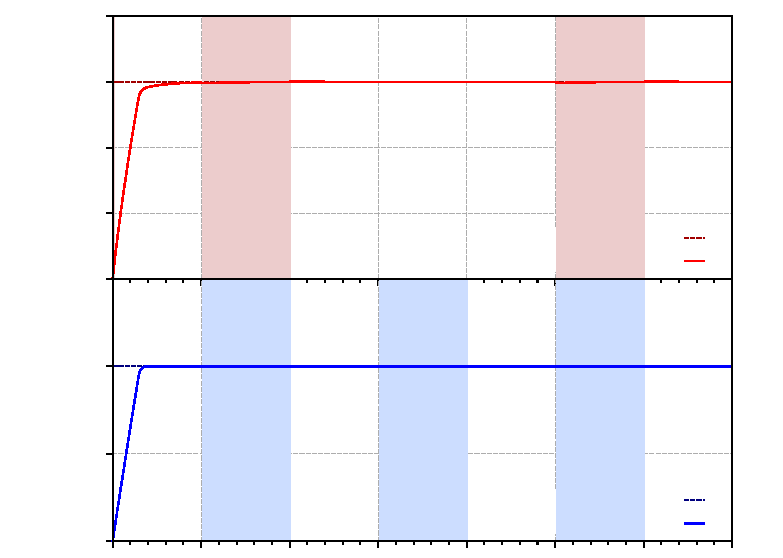
\includegraphics{fsivrgmp}}%
    \gplfronttext
  \end{picture}%
\endgroup

\vspace{1cm}
\caption{FSiVrGMP (90\%)}
\label{fig:fsivrgmp}
\end{figure}

\begin{figure}[htb]
\footnotesize
\centering
% GNUPLOT: LaTeX picture with Postscript
\begingroup
  \makeatletter
  \providecommand\color[2][]{%
    \GenericError{(gnuplot) \space\space\space\@spaces}{%
      Package color not loaded in conjunction with
      terminal option `colourtext'%
    }{See the gnuplot documentation for explanation.%
    }{Either use 'blacktext' in gnuplot or load the package
      color.sty in LaTeX.}%
    \renewcommand\color[2][]{}%
  }%
  \providecommand\includegraphics[2][]{%
    \GenericError{(gnuplot) \space\space\space\@spaces}{%
      Package graphicx or graphics not loaded%
    }{See the gnuplot documentation for explanation.%
    }{The gnuplot epslatex terminal needs graphicx.sty or graphics.sty.}%
    \renewcommand\includegraphics[2][]{}%
  }%
  \providecommand\rotatebox[2]{#2}%
  \@ifundefined{ifGPcolor}{%
    \newif\ifGPcolor
    \GPcolortrue
  }{}%
  \@ifundefined{ifGPblacktext}{%
    \newif\ifGPblacktext
    \GPblacktexttrue
  }{}%
  % define a \g@addto@macro without @ in the name:
  \let\gplgaddtomacro\g@addto@macro
  % define empty templates for all commands taking text:
  \gdef\gplbacktext{}%
  \gdef\gplfronttext{}%
  \makeatother
  \ifGPblacktext
    % no textcolor at all
    \def\colorrgb#1{}%
    \def\colorgray#1{}%
  \else
    % gray or color?
    \ifGPcolor
      \def\colorrgb#1{\color[rgb]{#1}}%
      \def\colorgray#1{\color[gray]{#1}}%
      \expandafter\def\csname LTw\endcsname{\color{white}}%
      \expandafter\def\csname LTb\endcsname{\color{black}}%
      \expandafter\def\csname LTa\endcsname{\color{black}}%
      \expandafter\def\csname LT0\endcsname{\color[rgb]{1,0,0}}%
      \expandafter\def\csname LT1\endcsname{\color[rgb]{0,1,0}}%
      \expandafter\def\csname LT2\endcsname{\color[rgb]{0,0,1}}%
      \expandafter\def\csname LT3\endcsname{\color[rgb]{1,0,1}}%
      \expandafter\def\csname LT4\endcsname{\color[rgb]{0,1,1}}%
      \expandafter\def\csname LT5\endcsname{\color[rgb]{1,1,0}}%
      \expandafter\def\csname LT6\endcsname{\color[rgb]{0,0,0}}%
      \expandafter\def\csname LT7\endcsname{\color[rgb]{1,0.3,0}}%
      \expandafter\def\csname LT8\endcsname{\color[rgb]{0.5,0.5,0.5}}%
    \else
      % gray
      \def\colorrgb#1{\color{black}}%
      \def\colorgray#1{\color[gray]{#1}}%
      \expandafter\def\csname LTw\endcsname{\color{white}}%
      \expandafter\def\csname LTb\endcsname{\color{black}}%
      \expandafter\def\csname LTa\endcsname{\color{black}}%
      \expandafter\def\csname LT0\endcsname{\color{black}}%
      \expandafter\def\csname LT1\endcsname{\color{black}}%
      \expandafter\def\csname LT2\endcsname{\color{black}}%
      \expandafter\def\csname LT3\endcsname{\color{black}}%
      \expandafter\def\csname LT4\endcsname{\color{black}}%
      \expandafter\def\csname LT5\endcsname{\color{black}}%
      \expandafter\def\csname LT6\endcsname{\color{black}}%
      \expandafter\def\csname LT7\endcsname{\color{black}}%
      \expandafter\def\csname LT8\endcsname{\color{black}}%
    \fi
  \fi
  \setlength{\unitlength}{0.0500bp}%
  \begin{picture}(7200.00,5040.00)%
    \gplgaddtomacro\gplbacktext{%
      \csname LTb\endcsname%
      \put(726,3150){\makebox(0,0)[r]{\strut{} 5}}%
      \csname LTb\endcsname%
      \put(726,3780){\makebox(0,0)[r]{\strut{} 10}}%
      \csname LTb\endcsname%
      \put(726,4409){\makebox(0,0)[r]{\strut{} 15}}%
      \csname LTb\endcsname%
      \put(726,5039){\makebox(0,0)[r]{\strut{} 20}}%
      \csname LTb\endcsname%
      \put(921,2237){\makebox(0,0){\strut{}}}%
      \csname LTb\endcsname%
      \put(1771,2237){\makebox(0,0){\strut{}}}%
      \csname LTb\endcsname%
      \put(2620,2237){\makebox(0,0){\strut{}}}%
      \csname LTb\endcsname%
      \put(3470,2237){\makebox(0,0){\strut{}}}%
      \csname LTb\endcsname%
      \put(4320,2237){\makebox(0,0){\strut{}}}%
      \csname LTb\endcsname%
      \put(5170,2237){\makebox(0,0){\strut{}}}%
      \csname LTb\endcsname%
      \put(6019,2237){\makebox(0,0){\strut{}}}%
      \csname LTb\endcsname%
      \put(6869,2237){\makebox(0,0){\strut{}}}%
      \put(352,3779){\rotatebox{-270}{\makebox(0,0){\strut{}Level [cm]}}}%
    }%
    \gplgaddtomacro\gplfronttext{%
      \csname LTb\endcsname%
      \put(6278,2913){\makebox(0,0)[r]{\strut{}Setpoint $T_1$}}%
      \csname LTb\endcsname%
      \put(6278,2693){\makebox(0,0)[r]{\strut{}Output $T_1$}}%
    }%
    \gplgaddtomacro\gplbacktext{%
      \csname LTb\endcsname%
      \put(726,0){\makebox(0,0)[r]{\strut{} 0}}%
      \csname LTb\endcsname%
      \put(726,840){\makebox(0,0)[r]{\strut{} 10}}%
      \csname LTb\endcsname%
      \put(726,1680){\makebox(0,0)[r]{\strut{} 20}}%
      \csname LTb\endcsname%
      \put(726,2520){\makebox(0,0)[r]{\strut{} 30}}%
      \csname LTb\endcsname%
      \put(921,-283){\makebox(0,0){\strut{}0}}%
      \csname LTb\endcsname%
      \put(1771,-283){\makebox(0,0){\strut{}15}}%
      \csname LTb\endcsname%
      \put(2620,-283){\makebox(0,0){\strut{}30}}%
      \csname LTb\endcsname%
      \put(3470,-283){\makebox(0,0){\strut{}45}}%
      \csname LTb\endcsname%
      \put(4320,-283){\makebox(0,0){\strut{}60}}%
      \csname LTb\endcsname%
      \put(5170,-283){\makebox(0,0){\strut{}75}}%
      \csname LTb\endcsname%
      \put(6019,-283){\makebox(0,0){\strut{}90}}%
      \csname LTb\endcsname%
      \put(6869,-283){\makebox(0,0){\strut{}105}}%
      \put(352,1260){\rotatebox{-270}{\makebox(0,0){\strut{}Level [cm]}}}%
      \put(3895,-613){\makebox(0,0){\strut{}Time [s]}}%
    }%
    \gplgaddtomacro\gplfronttext{%
      \csname LTb\endcsname%
      \put(6278,393){\makebox(0,0)[r]{\strut{}Setpoint $T_2$}}%
      \csname LTb\endcsname%
      \put(6278,173){\makebox(0,0)[r]{\strut{}Output $T_2$}}%
    }%
    \gplbacktext
    \put(0,0){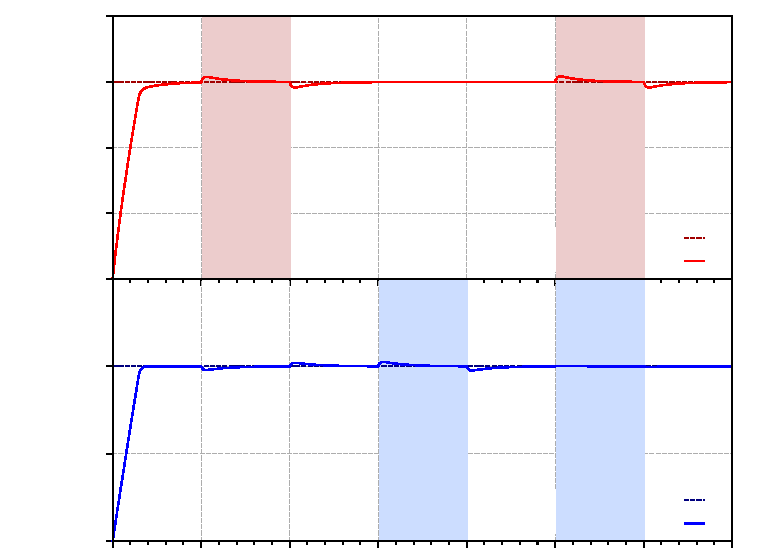
\includegraphics{fsieos}}%
    \gplfronttext
  \end{picture}%
\endgroup

\vspace{1cm}
\caption{FSiEOS (25\%)}
\label{fig:fsieos}
\end{figure}

\mychapter{Conclusões}
\label{cap:conclusoes}

% ------------------------------------------------------------------------------
\section{Trabalhos futuros}


\backmatter
% Apêndices --------------------------------------------------------------------
%\appendix
%\input{apendices/codigos}

% Bibliografia -----------------------------------------------------------------
\addcontentsline{toc}{chapter}{Referências Bibliográficas}
\bibliographystyle{ppgeec}
\bibliography{bibliografia}

% Fim do documento .............................................................
\end{document}
